% ******************************* PhD Thesis Template **************************
% Please have a look at the README.md file for info on how to use the template

\documentclass[a4paper,12pt,times,numbered,print,oneside,index,custombib]{Classes/PhDThesisPSnPDF}
%\usepackage[spanish]{babel}
%\usepackage[utf8]{inputenc}
%\selectlanguage{spanish}

% ******************************************************************************
% ******************************* Class Options ********************************
% *********************** See README for more details **************************
% ******************************************************************************

% `a4paper'(The University of Cambridge PhD thesis guidelines recommends a page
% size a4 - default option) or `a5paper': A5 Paper size is also allowed as per
% the Cambridge University Engineering Deparment guidelines for PhD thesis
%
% `11pt' or `12pt'(default): Font Size 10pt is NOT recommended by the University
% guidelines
%
% `oneside' or `twoside'(default): Printing double side (twoside) or single
% side.
%
% `print': Use `print' for print version with appropriate margins and page
% layout. Leaving the options field blank will activate Online version.
%
% `index': For index at the end of the thesis
%
% `draftclassic': For draft mode without loading any images (same as draft in book)
%
% `draft': Special draft mode with line numbers, images, and water mark with
% timestamp and custom text. Position of the text can also be modified.
%
% `abstract': To generate only the title page and abstract page with
% dissertation title and name, to submit to the Student Registry
%
% `chapter`: This option enables only the specified chapter and it's references
%  Useful for review and corrections.
%
% ************************* Custom Page Margins ********************************
%
% `custommargin`: Use `custommargin' in options to activate custom page margins,
% which can be defined in the preamble.tex. Custom margin will override
% print/online margin setup.
%
% *********************** Choosing the Fonts in Class Options ******************
%
% `times' : Times font with math support. (The Cambridge University guidelines
% recommend using times)
%
% `fourier': Utopia Font with Fourier Math font (Font has to be installed)
%            It's a free font.
%
% `customfont': Use `customfont' option in the document class and load the
% package in the preamble.tex
%
% default or leave empty: `Latin Modern' font will be loaded.
%https://v2.overleaf.com/project/5b7b5e3f7683327cf1b78585
% ********************** Choosing the Bibliography style ***********************
%
% `authoryear': For author-year citation eg., Krishna (2013)
%
% `numbered': (Default Option) For numbered and sorted citation e.g., [1,5,2]
%
% `custombib': Define your own bibliography style in the `preamble.tex' file.
%              `\RequirePackage[square, sort, numbers, authoryear]{natbib}'.
%              This can be also used to load biblatex instead of natbib
%              (See Preamble)
%
% **************************** Choosing the Page Style *************************
%
% `default (leave empty)': For Page Numbers in Header (Left Even, Right Odd) and
% Chapter Name in Header (Right Even) and Section Name (Left Odd). Blank Footer.
%
% `PageStyleI': Chapter Name next & Page Number on Even Side (Left Even).
% Section Name & Page Number in Header on Odd Side (Right Odd). Footer is empty.
%
% `PageStyleII': Chapter Name on Even Side (Left Even) in Header. Section Number
% and Section Name in Header on Odd Side (Right Odd). Page numbering in footer

% Uncomment to change page style
%\pagestyle{PageStyleII}

% ********************************** Preamble **********************************
% Preamble: Contains packages and user-defined commands and settings
% ******************************************************************************
% ****************************** Custom Margin *********************************

% Add `custommargin' in the document class options to use this section
% Set {innerside margin / outerside margin / topmargin / bottom margin}  and
% other page dimensions
\ifsetCustomMargin
  \RequirePackage[left=37mm,right=30mm,top=35mm,bottom=30mm]{geometry}
  \setFancyHdr % To apply fancy header after geometry package is loaded
\fi

% Add spaces between paragraphs
%\setlength{\parskip}{0.5em}
% Ragged bottom avoids extra whitespaces between paragraphs
\raggedbottom
% To remove the excess top spacing for enumeration, list and description
%\usepackage{enumitem}
%\setlist[enumerate,itemize,description]{topsep=0em}

% *****************************************************************************
% ******************* Fonts (like different typewriter fonts etc.)*************

% Add `customfont' in the document class option to use this section

\ifsetCustomFont
  % Set your custom font here and use `customfont' in options. Leave empty to
  % load computer modern font (default LaTeX font).
  %\RequirePackage{helvet}

  % For use with XeLaTeX
  %  \setmainfont[
  %    Path              = ./libertine/opentype/,
  %    Extension         = .otf,
  %    UprightFont = LinLibertine_R,
  %    BoldFont = LinLibertine_RZ, % Linux Libertine O Regular Semibold
  %    ItalicFont = LinLibertine_RI,
  %    BoldItalicFont = LinLibertine_RZI, % Linux Libertine O Regular Semibold Italic
  %  ]
  %  {libertine}
  %  % load font from system font
  %  \newfontfamily\libertinesystemfont{Linux Libertine O}
\fi

% *****************************************************************************
% **************************** Custom Packages ********************************

% ************************* Algorithms and Pseudocode **************************

%\usepackage{algpseudocode}


% ********************Captions and Hyperreferencing / URL **********************

% Captions: This makes captions of figures use a boldfaced small font.
%\RequirePackage[small,bf]{caption}

\RequirePackage[labelsep=space,tableposition=top]{caption}
\renewcommand{\figurename}{Fig.} %to support older versions of captions.sty


% *************************** Graphics and figures *****************************

%\usepackage{rotating}
%\usepackage{wrapfig}

% Uncomment the following two lines to force Latex to place the figure.
% Use [H] when including graphics. Note 'H' instead of 'h'
%\usepackage{float}
%\restylefloat{figure}

% Subcaption package is also available in the sty folder you can use that by
% uncommenting the following line
% This is for people stuck with older versions of texlive
%\usepackage{sty/caption/subcaption}
\usepackage{subcaption}

% ********************************** Tables ************************************
\usepackage{booktabs} % For professional looking tables
\usepackage{multirow}

%\usepackage{multicol}
%\usepackage{longtable}
%\usepackage{tabularx}


% *********************************** SI Units *********************************
\usepackage{siunitx} % use this package module for SI units


% ******************************* Line Spacing *********************************

% Choose linespacing as appropriate. Default is one-half line spacing as per the
% University guidelines

% \doublespacing
% \onehalfspacing
% \singlespacing


% ************************ Formatting / Footnote *******************************

% Don't break enumeration (etc.) across pages in an ugly manner (default 10000)
%\clubpenalty=500
%\widowpenalty=500

%\usepackage[perpage]{footmisc} %Range of footnote options


% *****************************************************************************
% *************************** Bibliography  and References ********************

%\usepackage{cleveref} %Referencing without need to explicitly state fig /table

% Add `custombib' in the document class option to use this section
\ifuseCustomBib
   \RequirePackage[square, sort, numbers, authoryear]{natbib} % CustomBib

% If you would like to use biblatex for your reference management, as opposed to the default `natbibpackage` pass the option `custombib` in the document class. Comment out the previous line to make sure you don't load the natbib package. Uncomment the following lines and specify the location of references.bib file

%\RequirePackage[backend=biber, style=numeric-comp, citestyle=numeric, sorting=nty, natbib=true]{biblatex}
%\bibliography{References/references} %Location of references.bib only for biblatex

\fi

% changes the default name `Bibliography` -> `References'
\renewcommand{\bibname}{References}


% ******************************************************************************
% ************************* User Defined Commands ******************************
% ******************************************************************************

% *********** To change the name of Table of Contents / LOF and LOT ************

%\renewcommand{\contentsname}{My Table of Contents}
%\renewcommand{\listfigurename}{My List of Figures}
%\renewcommand{\listtablename}{My List of Tables}


% ********************** TOC depth and numbering depth *************************

\setcounter{secnumdepth}{2}
\setcounter{tocdepth}{2}


% ******************************* Nomenclature *********************************

% To change the name of the Nomenclature section, uncomment the following line

%\renewcommand{\nomname}{Symbols}


% ********************************* Appendix ***********************************

% The default value of both \appendixtocname and \appendixpagename is `Appendices'. These names can all be changed via:

%\renewcommand{\appendixtocname}{List of appendices}
%\renewcommand{\appendixname}{Appndx}

% *********************** Configure Draft Mode **********************************

% Uncomment to disable figures in `draft'
%\setkeys{Gin}{draft=true}  % set draft to false to enable figures in `draft'

% These options are active only during the draft mode
% Default text is "Draft"
%\SetDraftText{DRAFT}

% Default Watermark location is top. Location (top/bottom)
%\SetDraftWMPosition{bottom}

% Draft Version - default is v1.0
%\SetDraftVersion{v1.1}

% Draft Text grayscale value (should be between 0-black and 1-white)
% Default value is 0.75
%\SetDraftGrayScale{0.8}


% ******************************** Todo Notes **********************************
%% Uncomment the following lines to have todonotes.

%\ifsetDraft
%	\usepackage[colorinlistoftodos]{todonotes}
%	\newcommand{\mynote}[1]{\todo[author=kks32,size=\small,inline,color=green!40]{#1}}
%\else
%	\newcommand{\mynote}[1]{}
%	\newcommand{\listoftodos}{}
%\fi

% Example todo: \mynote{Hey! I have a note}

% ************************ Thesis Information & Meta-data **********************
% Thesis title and author information, refernce file for biblatex
% ************************ Thesis Information & Meta-data **********************
%% The title of the thesis
\title{Sistema de Asistencia de Manejo para Optimización de Combustible en Buses de Transmisión Manual usando Machine Learning}
%\texorpdfstring is used for PDF metadata. Usage:
%\texorpdfstring{LaTeX_Version}{PDF Version (non-latex)} eg.,
%\texorpdfstring{$sigma$}{sigma}

%% Subtitle (Optional)
%\subtitle{}

%% Curso
\curso{Trabajo de Fin de Carrera (MTR280)}

%% The full name of the author
%% for multiple author, append each author with the \newline command
\author{Héctor David Aguirre Arista}
     
%% author Role (optional) - author (default) or leave empty
\authorrole{\textbf{Nombre: }}

%% author line width: required to align supervisors
\authorlinewidth{0.45\textwidth}

%% Department (eg. Department of Engineering, Maths, Physics)
\dept{Facultad de Ciencias e Ingeniería}

%% University and Crest
\university{Pontificia Universidad Católica del Perú}
% Crest minimum should be 30mm.
\crest{
\includegraphics[width=0.4\textwidth]{Figs/Logo_PUCP.png}}
%% Use this crest, if you are using the college crest
%% Crest long miminum should be 65mm
%\crest{
\includegraphics[width=0.45\textwidth]{University_Crest_Long}}

%% College shield [optional] 
% Crest minimum should be 30mm.
%\collegeshield{
\includegraphics[width=0.2\textwidth]{CollegeShields/Kings}}


%% Supervisor (optional)
%% for multiple supervisors, append each supervisor with the \newline command
\supervisor{Ericka Patricia Madrid Ruiz\newline
Elizabeth Roxana Villota Cerna}

%% Supervisor Role (optional) - Supervisor (default) or advisor
 \supervisorrole{\textbf{Profesores: }}
%% if no title is desired:
% \supervisorrole{}

%% Supervisor line width: required to align supervisors
\supervisorlinewidth{0.5\textwidth}

%% Advisor (optional)
%% for multiple advisors, append each advisor with the \newline command
\advisor{Jhon Portella Delgado}
     
%% Advisor Role (optional) - Advisor (default) or leave empty
 \advisorrole{\textbf{Asesor: }}
%% if no title is required
% \advisorrole{}

%% Advisor line width: required to align supervisors
\advisorlinewidth{0.45\textwidth}

%% codigo (optional)
%% for multiple codigo, append each codigo with the \newline command
\codigo{20131733}
     
%% codigo Role (optional) - codigo (default) or leave empty
\codigorole{\textbf{Código: }}

%% codigo line width: required to align supervisors
\codigolinewidth{0.45\textwidth}

%% horario (optional)
%% for multiple horario, append each horario with the \newline command
\horario{10M2}
     
%% horario Role (optional) - horario (default) or leave empty
\horariorole{\textbf{Horario: }}

%% horario line width: required to align supervisors
\horariolinewidth{0.45\textwidth}

%% You can redefine the submission text:
% Default as per the University guidelines:
% ``This dissertation is submitted for the degree of''
\renewcommand{\submissiontext}{}

%% Full title of the Degree
\degreetitle{}

%% College affiliation (optional)
%\college{King's College}

%% Submission date
% Default is set as {\monthname[\the\month]\space\the\year}
\degreedate{Noviembre 2018} 

%% Meta information
\subject{LaTeX} \keywords{{LaTeX} {Thesis} {Engineering} {Pontificia Universidad Católica del Perú}}


% ***************************** Abstract Separate ******************************
% To printout only the titlepage and the abstract with the PhD title and the
% author name for submission to the Student Registry, use the `abstract' option in
% the document class.

\ifdefineAbstract
 \pagestyle{empty}
 \includeonly{Declaration/declaration, Abstract/abstract}
\fi

% ***************************** Chapter Mode ***********************************
% The chapter mode allows user to only print particular chapters with references
% Title, Contents, Frontmatter are disabled by default
% Useful option to review a particular chapter or to send it to supervisior.
% To use choose `chapter' option in the document class

\ifdefineChapter
 \includeonly{Chapter3/chapter3}
\fi

% ******************************** Front Matter ********************************
\begin{document}

\frontmatter

\maketitle

%% ******************************* Thesis Dedidcation ********************************

\begin{dedication} 

I would like to dedicate this thesis to my loving parents \dots

\end{dedication}
%% ******************************* Thesis Declaration ***************************

\begin{declaration}

I hereby declare that except where specific reference is made to the work of 
others, the contents of this dissertation are original and have not been 
submitted in whole or in part for consideration for any other degree or 
qualification in this, or any other university. This dissertation is my own 
work and contains nothing which is the outcome of work done in collaboration 
with others, except as specified in the text and Acknowledgements. This 
dissertation contains fewer than 65,000 words including appendices, 
bibliography, footnotes, tables and equations and has fewer than 150 figures.

% Author and date will be inserted automatically from thesis.tex \author \degreedate

\end{declaration}
%% ************************** Thesis Acknowledgements **************************

\begin{acknowledgements}      


And I would like to acknowledge ...


\end{acknowledgements}

\setlength{\parskip}{0.5em}
% ************************** Thesis Abstract *****************************
% Use `abstract' as an option in the document class to print only the titlepage and the abstract.
\begin{abstract}
This is where you write your abstract ...
\end{abstract}
 %Este será ahora el resumen

% *********************** Adding TOC and List of Figures ***********************

\tableofcontents

\listoffigures

\listoftables

% \printnomenclature[space] space can be set as 2em between symbol and description
%\printnomenclature[3em]

\printnomenclature

% ******************************** Main Matter *********************************
\mainmatter


% ************************** Thesis Introduction *****************************
\begin{introduction}
%{El mundo en el que vivimos está cada vez más interconectado. En los últimos años se ha desarrollado tecnología que permite que objetos que antes simplemente operábamos, ahora se comuniquen e interactúen con nosotros de una manera más inteligente, que nos ahorra esfuerzos y mejora la calidad y seguridad de cada uno de ellos.
%Esto se ve claramente reflejado en el área automotriz, en la que muchas iniciativas por crear un auto autónomo están siendo desarrolladas.

En la actualidad vivimos con una importante preocupación, la contaminación ambiental. Las consecuencias que podría generar en nuestro planeta pueden ser muy graves. Una de las principales causas de la contaminación ambiental es la emisión de gases de efecto invernadero. El CO\textsubscript{2} es uno de estos gases y está presente en una de las actividades más cotidianas del mundo, El transporte.

Esta actividad está liderada por el uso de combustibles fósiles. Y aunque los autos eléctricos han empezado a ganar terreno en el sector automovilístico, estos aún representan tan solo el 1.3\% de las ventas totales de autos en el mundo. \mynote{Aquí falta poner la referencia} El transporte se registró como la fuente mas grande de emisión de CO\textsubscript{2} en el 2016 en Europa y Estados Unidos con el 27\% y 28\% de las emisiones de gases de efectos invernadero respectivamente.

Por otro lado, en el Perú la seguridad "vial" \mynote{Revisar este término} es un aspecto que preocupa a muchos peruanos. En el año 2017 murieron un total de 772 debido a accidentes de tránsito \mynote{Citar el comercio}. Esa no es una cifra despreciable. Las mayores causas de los accidentes de tránsito son el exceso de velocidad (32\%) y la imprudencia del conductor (28\%) \mynote{citar aquí al reporte estadístico PNP}. Estas dos causas son errores humanos que tienen mucho que ver con el estilo de manejo de los conductores. Cada conductor puede ejecutar una maniobra de manera muy agresiva como calmada y la agresividad en las maniobras no solo impacta en la seguridad vial, sino también en el consumo de combustible.

La presente tesis desarrollará un sistema que sea capaz de caracterizar el estilo de conducción de un usuario y que relacione ese estilo con su consumo de combustible. Se desarrollará un estilo de conducción ideal, que no sea muy agresivo y que sea lo mas eficiente posible.


\end{introduction}


%!TEX root = ../thesis.tex
%*******************************************************************************
%*********************************** First Chapter *****************************
%*******************************************************************************

\chapter{Planteamiento de la Problemática}  %Title of the First Chapter

\ifpdf
    \graphicspath{{Chapter1/Figs/Raster/}{Chapter1/Figs/PDF/}{Chapter1/Figs/}}
\else
    \graphicspath{{Chapter1/Figs/Vector/}{Chapter1/Figs/}}
\fi


%********************************** %First Section  **************************************
\section{Motivación General}



\section{Motivación Específica y Propuesta de Solución}

%!TEX root = ../thesis.tex
%*******************************************************************************
%****************************** Second Chapter *********************************
%*******************************************************************************

\chapter{Estado del Arte}

\ifpdf
    \graphicspath{{Chapter2/Figs/Raster/}{Chapter2/Figs/PDF/}{Chapter2/Figs/}}
\else
    \graphicspath{{Chapter2/Figs/Vector/}{Chapter2/Figs/}}
\fi

\section{Términos relacionados con el estilo de conducción}

El concepto de "Estilo de conducción" no tiene una definición estándar que sea aceptada en todo el mundo. Al contrario, este concepto involucra una serie de factores que aumentan su complejidad y complican su definición. Debido a esto se usarán los conceptos definidos por \citeauthor{8002632} \cite{8002632}.

\begin{figure}[htbp!]
\centering

\includegraphics[width=0.8\textwidth]{Fig1}
\caption[Terminología estilo de conducción]{Terminología relacionada con el estilo de conducción \cite{8002632}}
\label{fig:2.1}
\end{figure}

Como se aprecia en la Fig~\ref{fig:2.1}, se entiende por un evento de conducción como las maniobras que se usan durante la acción de conducir, como por ejemplo: acelerar, desacelerar y girar.

De la misma manera, El patrón de conducción se define como el resultado de los eventos de conducción sujetos a condiciones de manejo, como el clima o el tipo de calzada. Este resultado se puede expresar como un perfil de velocidades. en el que están incluidos todos los datos que se pueden obtener partiendo de este perfil de velocidad, como por ejemplo: duración del viaje, velocidad promedio y demanda de potencia calculada.

La habilidad de conducción es la habilidad que posee el conductor para controlar el vehículo. Este concepto se usa para diferenciar entre un conductor experimentado o profesional de un conductor promedio.

El estilo de conducción es más complejo de definir debido a que para algunos autores involucra factores subjetivos como la actitud del conductor, el humor o el cansancio. Para \citeauthor{6957822} \cite{6957822}, el estilo de conducción  es la manera en la que la tarea de conducción es realizada. Esto se traduce en la forma en la que el conductor opera el vehículo (Pedal de aceleración, timón, freno, etc.). Esto se diferencia de el patrón de conducción tan solo porque no se asocia con un recorrido en especifico sino con un conductor.

También, se puede expresar el estilo de conducción en niveles de agresividad como \citeauthor{6294318} \cite{6294318}. Debido a que la agresividad en los eventos de conducción esta asociada con un mayor consumo de combustible y a menor seguridad vial, definitivamente juega un papel importante dentro del concepto de estilo de conducción. Esta es la forma en la que se definirá el estilo de conducción para esta tesis.

\section{Estado del arte según algoritmos usados}
Se procederá a mostrar las implementaciones e investigaciones desarrolladas en la actualidad clasificados según el tipo de algoritmo que se uso para la caracterización de el estilo de conducción

\subsection{Algoritmos basados en reglas}
Dentro de esta categoría se encuentran algoritmos de clasificación basados en reglas que comprenden el uso de lógica difusa, lógica difusa adaptativa y algoritmos de agrupamiento. Estos algoritmos se caracterizan por estar definidos por {\it umbrales predefinidos} y son el enfoque más sencillo para tratar de clasificar los estilos de conducción.

\citeauthor{6957822} \cite{6957822} desarrolló un sistema de reconocimiento de estilo de conducción online usando lógica difusa. Este sistema esta implementado usando {\it Matlab/Simulink}  y es paramétrico, Se puede configurar para ser usado en distintos tipos de vehículos.
El sistema detecta la aceleración longitudinal, aceleración lateral, desaceleración, velocidad, brecha de tiempo y activación del sistema autónomo de velocidad crusero. Además determina a través de un Sistema de Navegación el tipo de calzada en el que se encuentra (Se distingue entre trocha, calles urbanas, carreteras pavimentadas y carreteras rurales). Esto lo realiza debido a que el tipo de calzada influencia en gran medida al estilo de conducción. Por ejemplo, en una trocha la mayoría de conductores manejarían a una velocidad suave para no dañar al vehículo, lo cuál no necesariamente quiere decir que el mismo conductor conduzca de esa manera en otro tipo de escenarios.
Usando Lógica Difusa se definieron 3 niveles de estilo de conducción: {\it Normal, Confortable y Deportivo}. Se probó el sistema en una simulación y se obtuvieron los siguientes resultados promedio (Fig.~\ref{fig:2.2}): 67.8\% de clasificaciones correctas y solo 2\% de clasificaciones incorrectas (El otro 30.2\% pertenece a clasificaciones "Diferentes" que dan una clasificación contigua de estilo de manejo, por ejemplo cuando la clasificación real es {\it Normal} pero el sistema arroja como resultado {\it Confortable}, en cambio las clasificaciones incorrectas dan un resultado no contiguo al real)

\begin{figure}[htbp!]
\centering
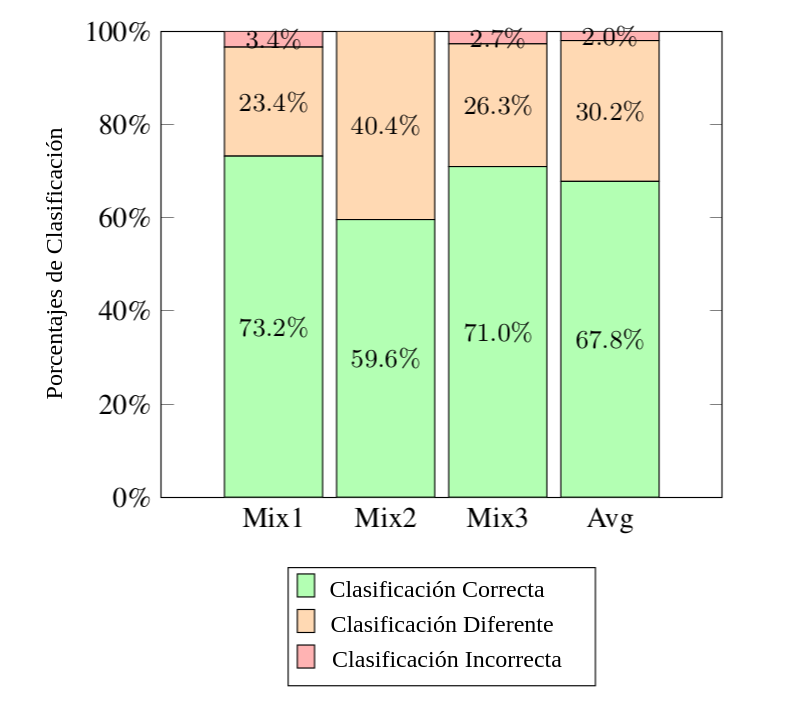
\includegraphics[width=0.8\textwidth]{Fig2}
\caption[Resultados del sistema de reconocimiento de estilo de conducción]{Resultados del sistema de reconocimiento de estilo de conducción en \cite{6957822}}
\label{fig:2.2}
\end{figure}

Usar lógica difusa no es la única manera de clasificar estilos de conducción. \citeauthor{4938719} \cite{4938719} presentó un método de clasificación basado en el análisis del perfil de la sobreaceleración (la derivada de la aceleración respecto al tiempo). En su investigación define al estilo de manejo como un comportamiento dinámico, Un conductor puede manejar de forma calmada por un momento y de forma agresiva en otro momento. Por este motivo, el método de clasificación que propone predice el estilo de conducción del usuario en tiempo real.
El algoritmo funciona de la siguiente manera:
\begin{enumerate}
    \itemsep0em
    \item Calcula el perfil de sobreaceleración durante una ventana de tiempo predefinido.
    \item Calcula la desviación estándar de la sobreaceleración durante toda la ventana de tiempo.
    \item Detecta el tipo de calzada actual y el nivel de congestión de tráfico usando el algoritmo propuesto en \cite{Highway_cap_manual}.
    \item Calcula la proporción de sobreaceleración dividiendo la desviación estándar con un valor promedio que depende de el tipo de calzada y el nivel de tráfico actuales.
    \item Dependiendo del resultado de la división realizada el conductor puede ser clasificado como {\it Calmado, Normal} o {\it Agresivo} usando reglas con umbrales predefinidos.
\end{enumerate}
\begin{figure}[htbp!]
\centering
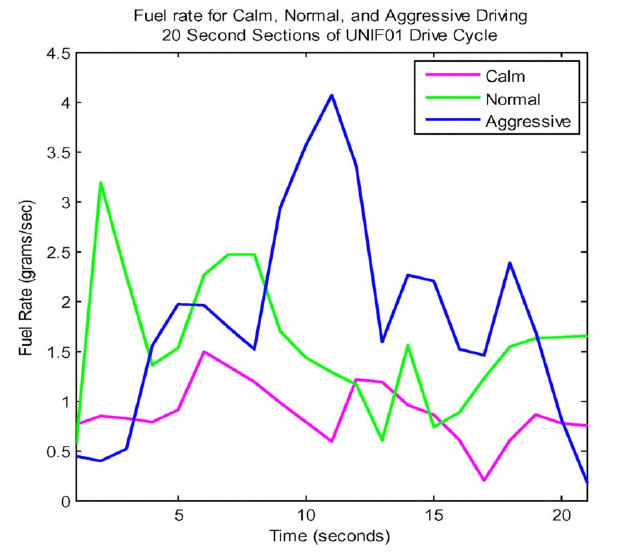
\includegraphics[width=0.75\textwidth]{Fig3}
\caption[Tasa de consumo de combustible según diferentes estilos de conducción]{Tasa de consumo de combustible según diferentes estilos de conducción \cite{4938719}.}
\label{fig:2.3}
\end{figure}
Este resultado dependerá mucho de la duración definida para la ventana de tiempo. Se recomendó usar una ventana de duración de 6 a 9 segundos para detectar los cambios de estilo de conducción oportunamente.

Se realizó también una comparación entre los 3 diferentes estilos de conducción con respecto a la tasa de consumo de combustible. Como se puede apreciar en la Fig.~\ref{fig:2.3}, los conductores clasificados como calmados están asociados a un menor consumo de combustible, mientras que los agresivos a un mayor consumo de combustible.

%para optimizar el uso de combustible. Por ejemplo en un vehículo híbrido, si el sistema predice que el conductor manejará de una manera agresiva, el sistema usará más potencia del motor eléctrico que del de combustión para así ayudar al ahorro de combustible.

Se ha presentado dos algoritmos basados en reglas que usan tanto múltiples variables \cite{6957822} como una sola \cite{4938719} para predecir el estilo de conducción del usuario. Sin embargo, los resultados de estos sistemas dependen en gran medida del valor de los umbrales escogidos para realizar la clasificación.

\subsection{Algoritmos basados en datos}
Cuando se tiene una cantidad muy grande de datos, es difícil analizarlos para obtener las reglas que guíen al algoritmo. Es entonces cuando los algoritmos basados en datos entran en acción. Estos algoritmos, en comparación con los basados en reglas, pueden manejar una mayor cantidad de datos y deducir umbrales consistentes con estos datos sin que estos dependan de un experto en el tema. A continuación se presentarán los distintos tipos de algoritmos basados en datos y su uso en el reconocimiento de estilos de conducción.

%********* Reinicia la cuenta de los \subsubsection y coloca el formato A,B,..****************************
\counterwithout{subsubsection}{subsection}
\renewcommand{\thesubsubsection}{\Alph{subsubsection}}
%********************************************************************************************************

\subsubsection{Algoritmos de aprendizaje de máquinas no supervisados}
Los algoritmos no supervisados no necesitan que los datos obtenidos por medio de los sensores en la actividad de conducción estén etiquetados. Es decir, si se registra los datos de un ciclo de conducción para un conductor, este registro no necesita estar asociado con el estilo de conducción que mantuvo este conductor. Esta clase de algoritmos busca patrones en los datos y los segrega teniendo en cuenta sus similitudes y diferencias en diferentes grupos sin etiquetar.

\citeauthor{constantinescu} \cite{constantinescu} propuso el análisis de el estilo de conducción por medio de dos algoritmos: Hierarchical Cluster Analysis (HCA) y Principal Component Analysis (PCA).

HCA es un algoritmo de {\it machine learning} que trata de categorizar a cada individuo en grupos con características similares. Es muy útil cuando no se conoce con exactitud el número de grupos. Por medio de un análisis estadístico trata de minimizar la varianza dentro de cada grupo y a la vez aumentarla entre diferentes grupos. En este caso, el algoritmo de agrupamiento jerárquico consiste en empezar con grupos consistentes de un solo miembro y consecutivamente ir combinando los dos grupos más cercanos, hasta solo tener un grupo.

PCA es un método estadístico que usa una trasformación para convertir un posible conjunto de variables relacionadas entre si en otro conjunto menor de variables linealmente independientes, en las que la varianza sea maximizada.

Para este caso en particular se trabajo con dispositivo GPS que se encargaba de medir la velocidad y aceleración del vehículo monitorizado a una frecuencia de muestreo de \SI[mode=text]{1}{Hz}. De esta data se escogieron los siguientes parámetros:
\begin{enumerate}
    \itemsep0em
    \item Velocidad por encima de los \SI[mode=text]{60}{Km/h}.
    \item Velocidad promedio.
    \item Desviación estándar de la velocidad.
    \item Desviación estándar de la aceleración.
    \item Promedio de la aceleración positiva.
    \item Desviación estándar de la aceleración positiva.
    \item Promedio de la aceleración negativa o frenado.
    \item Desviación estándar del frenado.
    \item Trabajo mecánico, que se calculó sumando toda la energía cinética positiva requerida para aumentar la velocidad del vehículo.
\end{enumerate}

Luego del análisis realizado se encontraron 6 grupos o clusters y se describió cada uno de estos como se puede observar en el Tabla~\ref{diag:2.1} usando los 5 componentes principales resultantes al aplicar PCA.

\begin{table}[htbp!]
\centering
\caption[Descripción de los clusters obtenidos]{Descripción de los clusters obtenidos en \cite{constantinescu}.}
\begin{tabular}{crrrr}
\toprule
\multicolumn{1}{l}{\textbf{Cluster}} & \multicolumn{1}{c}{\textbf{Agresividad}} & \multicolumn{1}{c}{\textbf{Velocidad}} & \multicolumn{1}{c}{\textbf{Aceleración}} & \multicolumn{1}{c}{\textbf{Frenado}} \\ \midrule
1 & Moderadamente baja & Baja-Moderada & Moderada & Suave-Moderado \\
2 & Muy baja & Baja-Moderada & Baja-Moderada & Suave-Moderado \\
3 & Moderadamente alta & Moderada & Moderada & Repentino \\
4 & Neutral & Moderada & Alta & Moderado \\
5 & Neutral & Moderada-Alta & Baja-Moderada & Moderado-Repentino \\
6 & Alta & Alta & Alta & Repentino \\ \bottomrule
\end{tabular}
\label{diag:2.1}
\end{table}

Los algoritmos no supervisados tienen una gran ventaja, no se necesitan conocer las etiquetas de clasificación {\it a priori}. Esto significa que la definición de etiquetas no limita o influencia de alguna manera a los resultados obtenidos, ya que los grupos o clusters formados dependen solo de los datos usados. Sin embargo, luego de hallar los grupos se necesita realizar un análisis para determinar su naturaleza.

\subsubsection{Algoritmos de aprendizaje de máquinas supervisados}

Los algoritmos supervisados, a diferencia de los no supervisados, necesitan tener un conocimiento previo de los datos que se tienen. Es decir, cada uno de los datos recolectados deben estar asociados a una etiqueta o clase ya predefinida.

Uno de los algoritmos más utilizados es el de K-Nearest Neighbors (k-NN), que se utilizó junto a Dynamic Time Warping (DTW) en el sistema de reconocimiento propuesto por \citeauthor{6083078} \cite{6083078}. El objetivo de este sistema es reconocer maniobras agresivas para dar un feedback al conductor y monitorizarlo, mejorando así la seguridad vial. Para lograrlo usaron los sensores presentes en un smartphone (acelerómetro, giroscopio, GPS y cámara frontal). Este sistema trabaja grabando la información de todos los sensores durante 5 minutos, luego analiza si ha ocurrido alguna maniobra potencialmente agresiva. Si una maniobra de este tipo ocurrió, conserva la información para un análisis posterior. En cambio, si no ocurrió ninguna maniobra de este tipo, borra la data para ahorrar espacio en disco.

Para la clasificación de cada maniobra detectada se usa Dynamic Time Warping (DTW), el cual es un algoritmo que es capaz de analizar la similaridad entre dos señales que no necesariamente tengan la misma duración y probablemente tengan un desfase. En la Fig.~\ref{fig:2.4} se puede observar una comparación entre una comparación de una distancia Euclidiana y otra usando DTW en dos señales muy parecidas en forma pero que no se encuentran en fase.


\begin{figure}[htbp!]
\centering
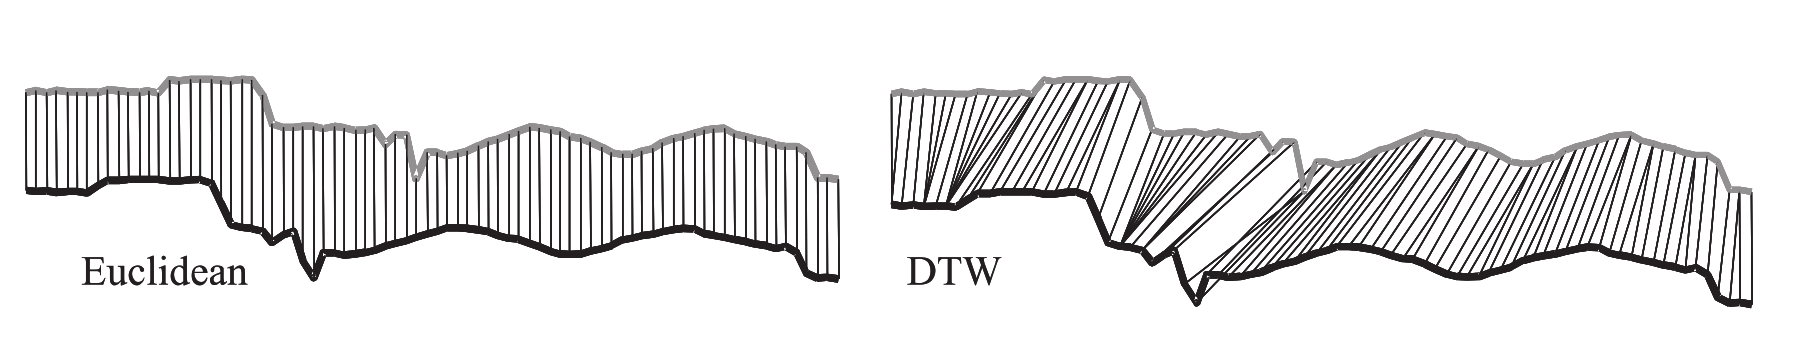
\includegraphics[width=0.95\textwidth]{Fig4}
\caption[Comparación de señales usando distancia Euclidiana y DTW]{Comparación de señales usando distancia Euclidiana y DTW \cite{Keogh2005}.}
\label{fig:2.4}
\end{figure}

El algoritmo consiste en crear una matriz de deformación $n \times m$, siendo $n$ y $m$ los números de puntos en cada señal. Esta matriz se llena calculando distancias entre cada punto, sin importar si se encuentran en el mismo instante temporal. Luego se dibuja el camino con la distancia más corta que une el inicio de las señales con el final de estas Fig.~\ref{fig:2.5} {\bf (B)}. La suma de distancias en este camino se define como la distancia entre las dos señales analizadas y se puede usar para comparar la similitud y clasificar señales usando modelos. Información detallada sobre este algoritmo se puede encontrar en \cite{Keogh2005}.
\begin{figure}[htpb!]
\centering
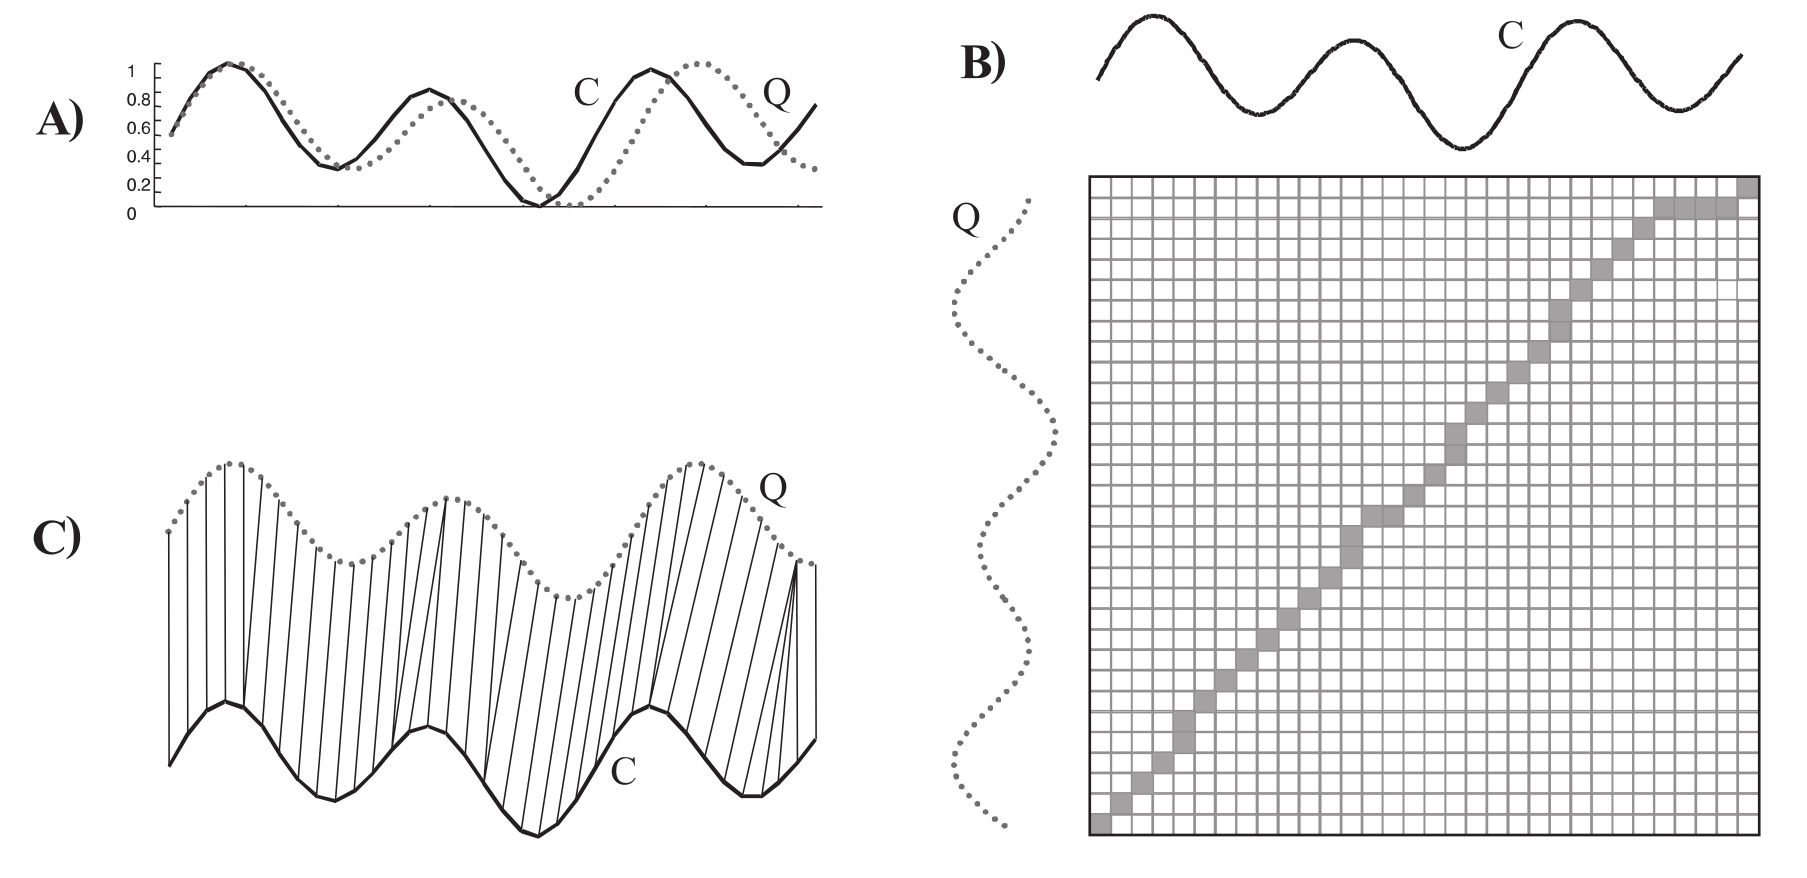
\includegraphics[width=0.85\textwidth]{Fig5}
\caption[Algoritmo de {\it Dynamic Time Warping}]{{\bf A)} Dos señales con forma muy similar pero desfasadas. {\bf B)} Matriz de deformación usada para encontrar el camino de deformación. {\bf C)} El resultado del alineamiento y deformación usando DTW. \cite{Keogh2005}.}
\label{fig:2.5}
\end{figure}

Para poder usar DTW se necesitó contar con señales modelo para cada tipo de maniobra a detectar. Se tuvo un total de 120 señales modelo en total, cada una asociada con una maniobra específica.  Usando DTW se puede obtener una medida de distancia entre las señales a clasificar y las señales modelo. Luego se aplicó K-Nearest Neighbors (k-NN) para clasificar cada señal. Lo que hace k-NN es tener en guardadas las señales modelos y al momento de clasificar una nueva señal calcula la distancia con las señales modelos, selecciona las $k$ distancias menores y dependiendo de la clase que tenga más señales cercanas, esta nueva señal es clasificada.

Para realizar la clasificación de señales solo se utilizó los datos de $g_x$, $a_y$ y $e_x$ (giroscopio en $x$, aceleración en $y$ y ángulo de rotación de Euler en $x$ respectivamente). Se puede observar en el Tabla.~\ref{diag:2.2} los porcentajes de reconocimiento exitoso por cada maniobra.

% Please add the following required packages to your document preamble:
% \usepackage{booktabs}
\begin{table}[htbp!]
\centering
\caption[Porcentaje de reconocimiento de maniobras de conducción]{Porcentaje de reconocimiento exitoso de maniobras de conducción \cite{6083078}.}
\begin{tabular}{@{}lc@{}}
\toprule
Maniobra & \multicolumn{1}{l}{\begin{tabular}[c]{@{}l@{}}Porcentaje de reconocimiento exitoso (\%)\end{tabular}} \\ \midrule
Giro a la derecha (\ang{90}) & 92 \\
Giro a la izquierda (\ang{90}) & 83 \\
Vuelta en U (\ang{180}) & 77 \\
Giro a la derecha agresivo & 100 \\
Giro a la izquierda agresivo & 100 \\
Vuelta en U agresiva & 100 \\
Cambio de carril agresivo (derecha) & 100 \\
Cambio de carril agresivo (izquierda) & 83 \\ \bottomrule
\end{tabular}
\label{diag:2.2}
\end{table}

Otro algoritmo aplicado usualmente al reconocimiento de estilos de manejo es el uso de {\it Redes Neuronales}. \citeauthor{7727682} \cite{7727682} utilizó redes neuronales para clasificar estilos de manejo y {\it Algoritmos Genéticos} para optimizar estas redes e incluso elegir los parámetros de entrada. El sistema que propuso se enfocaba en obtener un clasificador que pueda ser utilizado por un sistema embebido de potencia baja. Por lo cuál utilizo un tipo de red neuronal llamado {\it Extreme Learning Machines}. Este tipo de red neuronal, como se observa en la Fig.~\ref{fig:2.6}, se caracteriza por tener tan solo una capa oculta entre las entradas y las salidas. Además se eligen los pesos entre las entradas y la única capa oculta de manera aleatoria y nunca se actualizan. Esta red neuronal solo aprende los pesos entre la capa oculta y las salidas en una sola iteración. Por esta razón este tipo de red resulta siendo muy ligero y de entrenamiento muy veloz.

\begin{figure}[htpb!]
\centering
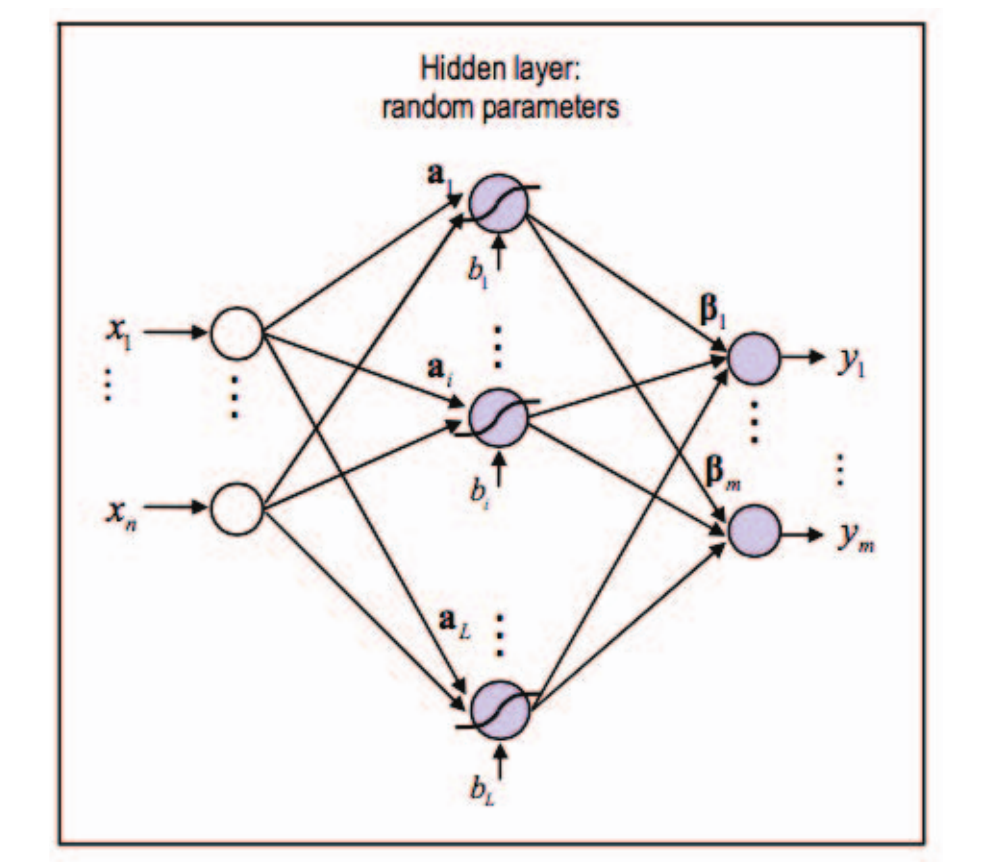
\includegraphics[width=0.8\textwidth]{Fig6}
\caption[Topología de una Red Neuronal usada para Extreme Learning Machines]{Topología de una Red Neuronal usada para Extreme Learning Machines \cite{7727682}.}
\label{fig:2.6}
\end{figure}

\citeauthor{7727682} recolectó un conjunto de 21 variables de 11 conductores, pero no utilizó toda la información. En lugar de eso utilizó un algoritmo genético llamado {\it Non-Dominated Sorting Genetic Algorithm}. Este tipo de algoritmo genético realiza una optimización multiobjetivo. Lo cual significa que trata de optimizar más de una variable a la vez. En este caso se trata de minimizar 3 variables: el número de atributos de entrada para la red neuronal, el número de neuronas en la capa oculta y la tasa de error resultante de la red neuronal entrenada.

Normalmente no existe una solución que permita minimizar las 3 variables a la vez. Debido a esto, lo que se busca en realidad se conoce como {\it Soluciones Óptimas de Pareto}. Este término hace referencia a las soluciones en las que no se puede optimizar ninguna variable sin degradar a otra. Este tipo de algoritmos genéticos contiene el concepto de Soluciones óptimas de Pareto como función de fitness, de tal manera que permite optimizar las 3 variables antes mencionadas.

Finalmente, se escoge una solución que tiene un 90.1\% de tasa de reconocimiento, 8 entradas para la red neuronal y 16 neuronas en la capa oculta.

\subsubsection{Algoritmos que combinan los enfoques supervisados y no supervisados}

Los algoritmos supervisados y no supervisados aparecen como dos categorías totalmente separadas. Sin embargo, esto no significa que no se puedan usar juntos y combinar para mejorar sus ventajas o reducir sus desventajas.

\citeauthor{6629603} \cite{6629603} propuso un sistema
que utiliza los sensores inerciales embebidos en un auto para identificar posibles maniobras inseguras y proporcionar un adecuado feedback hacia el conductor. Además también propone caracterizar y diferenciar conductores solo usando datos de los sensores inerciales, para poder diferenciar cuando dos personas distintas utilizan un mismo vehículo. Para lograr su objetivo primero analiza la información de los sensores para determinar un conjunto básico de maniobras: frenado, aceleración y giro.


Se utiliza el algoritmo de aprendizaje no supervisado {\it K-means Clustering} para identificar las maniobras. Este algoritmo consiste en generar $k$ semillas, de preferencia no aleatorias ya que la inicialización tiene una gran influencia en los clusters resultantes, que representarán la media o el centroide de cada cluster, luego por medio de la definición de una métrica de distancia (Euclidiana, citiblock, etc.) se asignan los datos al cluster del centroide más cercano. Luego de clasificar a todos los datos se vuelve a calcular el centroide de cada cluster (que muy probablemente cambiará de posición) y se repite los pasos hasta converger en una posición de centroides.


Al identificar las maniobras se usan dos fuentes de datos distintas: la primera cuenta con la inforamcion completa de los sensores, asi como también un análisis estadístico de estos (mínimo, máximo, media, varianza, etc.); en cambio, la segunda solo cuenta con el análisis estadístico. Y los resultados que se obtienen son muy similares. El desempeño de el clasificador no se reduce al no incluir los datos completos de los sensores, sino que puede usar tan solo sus datos estadísticos.

Luego se utiliza el algoritmo supervisado {\it Support Vector Machines} (SVM). Este algoritmo usa los datos con sus respectivas clases y trata de crear un hiperplano que separe todos los datos pertenecientes a una clase de la otra. Mientras este hiperplano tenga una mayor distancia con los miembos más cercanos de ambas clases, se tendrá un menor error de generalización. El encontrar este hiperplano que separe a las dos clases en la mayoría de los casos no es posible en el espacio definido por los atributos actuales de los datos. Debido a esto se mapean los datos en un espacio con más dimensiones para lograr encontrar este hiperplano de una manera más sencilla.

\section{Estado del arte según sensores usados}

Para usar los algoritmos mencionados anteriormente se han usado diferentes clases de sensores para medir distintas variables, ya sea directa o indirectamente. En el Tabla~\ref{diag:2.3} se puede apreciar los sensores utilizados en las investigaciones mencionadas.

\begin{table}[htpb!]
\centering
\caption{Resumen de sensores usados en las investigaciones mencionadas}
\begin{tabular}{@{}ll@{}}
\toprule
Sensores usados & Referencias \\ \midrule
Inertial Measurement Unit (IMU)& \cite{4938719}, \cite{7727682}, \cite{6629603} \\
Acelerómetros de bajo costo & \cite{6294318} \\
Smartphone & \cite{6083078} \\
GPS & \cite{constantinescu} \\
GPS e IMU & \cite{6957822} \\ \bottomrule
\end{tabular}
\label{diag:2.3}
\end{table}

\subsection{Inertial Measurement Unit}
Esta clase de sensores se puede encontrar bajo un rango de precios muy amplio. Existen unidades por debajo de los \textdollar 10 como el MPU-6050 (Fig.~\ref{fig:2.7}) que cuenta con un giroscopio de 3 ejes, un acelerómetro de 3 ejes y funciona a un voltaje de \SI[mode=text]{2.3}{V} a \SI[mode=text]{3.4}{V} \cite{invensense}

\begin{figure}[htpb!]
\centering
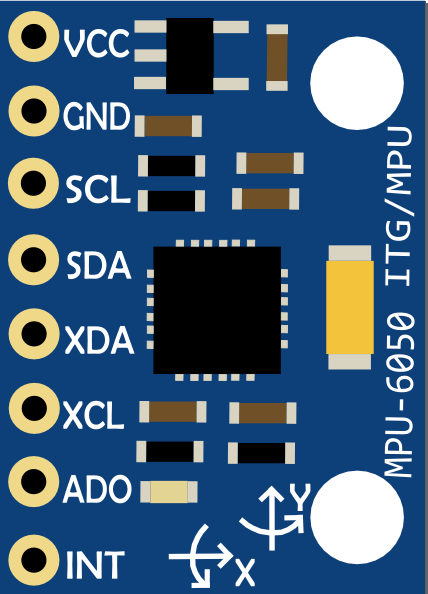
\includegraphics[width=0.3\textwidth]{Fig7}
\caption[MPU-5050 de Invensense]{MPU-5050 de Invensense \cite{invensense}.}
\label{fig:2.7}
\end{figure}

%!TEX root = ../thesis.tex
%*******************************************************************************
%****************************** Third Chapter **********************************
%*******************************************************************************
\chapter{Diseño Conceptual}

% **************************** Define Graphics Path **************************
\ifpdf
    \graphicspath{{Chapter3/Figs/Raster/}{Chapter3/Figs/PDF/}{Chapter3/Figs/}}
\else
    \graphicspath{{Chapter3/Figs/Vector/}{Chapter3/Figs/}}
\fi

\section{Requerimientos del sistema}
Uno de los requerimientos principales del sistema es el uso de una red de sensores modular y sencilla de instalar en distintos tipos de vehículos. Esto se explica fácilmente debido a que este sistema esta orientado a ser usado en el sistema de transporte público en Lima, el cual tiene una gran variedad y un gran número de vehículos. El sistema, entonces, debe ser adaptable a cualquiera de estos vehículos y no contar con un tiempo de instalación elevado.

También se tiene como requerimiento un grado de precisión alto en el reconocimiento de estilos y eventos de conducción. Esto es necesario debido a que este sistema se usará para monitorizar y mejorar la conducta de conducción de los choferes del servicio de transporte público. Los datos arrojados por este sistema necesitan ser confiables.

Por último, se necesita también de una adecuada infraestructura que permita que el sistema funcione en linea, entregando feedback al conductor, aún si se presentan condiciones como la falta temporal de conexión a Internet. Este requerimiento será importante al considerar donde realizar el procesamiento de los datos (dentro de un sistema embebido en cada vehículo o usando un servidor).

\bgroup
\def\arraystretch{1.5}%  1 is the default, change whatever you need
\begin{table}[hpbt!]
\centering
\caption{Lista de exigencias}
\resizebox{\textwidth}{!}{%
\begin{tabularx}{\textwidth}{|l|X|}
\hline
\multicolumn{2}{|c|}{\textbf{Lista de exigencias}} \\ \hline
\textbf{Tema:} & Sistema de Reconocimiento de Estilo de Conducción para Optimización de consumo de Combustible en Vehículos del Sistema de Transporte Público de Lima \\ \hline
\textbf{Categoría} & \multicolumn{1}{c|}{\textbf{Descripción}}  \\ \hline
Función Principal & Reconocer el estilo de manejo de un conductor del sistema de transporte público de Lima y otorgarle un feedback adecuado. \\ \hline
Seguridad & El sistema no deberá influir en elementos que puedan generar un accidente de tránsito, como la visibilidad a través del parabrisas o a través de los espejos. \\ \hline
Señales & El sistema contará con una conexión a Internet permanente, con la cual guardará la información recolectada. \\ \hline
Energía & El sistema funcionará a través de una batería de larga duración, que tenga la posibilidad de recargarse usando como fuente de energía al vehículo. \\ \hline
Geometría & Las medidas del sistema no deberán superar los \SI{30}{cm} de altura o de largo y ancho \\ \hline
Peso & El peso del módulo debe ser menor que \SI{1}{Kg}.\\ \hline
Electrónica & Se empleará sensores que puedan detectar información relevante para el reconocimiento de estilo de manejo y un sistema de feedback para informal al conductor. \\ \hline
Software & Se desarrollará una plataforma en la que se permita obtener los datos medidos por el sistema de una forma sencilla. \\ \hline
Mantenimiento & Se deberá realizar un mantenimiento preventivo del sistema cada 6 meses, para asegurar su funcionamiento. \\ \hline
Ergonomía & El sistema de sensores deberá estar en una posición que no afecte a la actividad de conducción y el sistema de feedback debe estar en una posición en la que el conductor pueda recibir el feedback sin comprometer la visibilidad de la tarea de conducción. \\ \hline
Transporte & El sistema será sencillo de instalar y desinstalar, para su uso en un número grande de vehículos \\ \hline
Uso & El sistema deberá usarse durante toda la tarea de conducción a temperatura ambiente y protegido de condiciones climáticas adversas. \\ \hline
Tiempo de entrega & El diseño deberá ser finalizado junto a los documentos correspondientes antes de la semana 15 del presente ciclo académico. \\ \hline
\end{tabularx}%
}
\label{diag:3.1}
\end{table}
\egroup

 \chapter{Diseño del sistema mecatrónico }

 En este capítulo se desarrollará el diseño del sistema a partir del concepto óptimo de solución desarrollado en el capítulo anterior. Para comenzar, se presenta el sistema integrado en su totalidad y se describe su funcionamiento. Luego, se presentará el desarrollo del sistema electrónico. El cuál comprende la selección de componentes, los diagramas esquemáticos y el desarrollo de la placa electrónica. A continuación, se presentará el diseño mecánico. El cuál consiste de cálculos básicos, selección de componentes y materiales y descripción de planos de ensamble y despiece. Por último, se presentará el diseño del algoritmo de clasificación. El cuál incluye los diagramas de flujo que describen los algoritmos utilizados. Las hojas de datos y planos completos se pueden encontrar en los Anexos
 %******************* Aquí falta indicar que anexos*******************************

 \graphicspath{{Chapter4/Figuras/}{Chapter4/Figs/PDF/}{Chapter4/Figs/}{Chapter4/segundo/}}

\section{Integración del sistema mecatrónico}

\begin{figure}[htbp!]
\centering
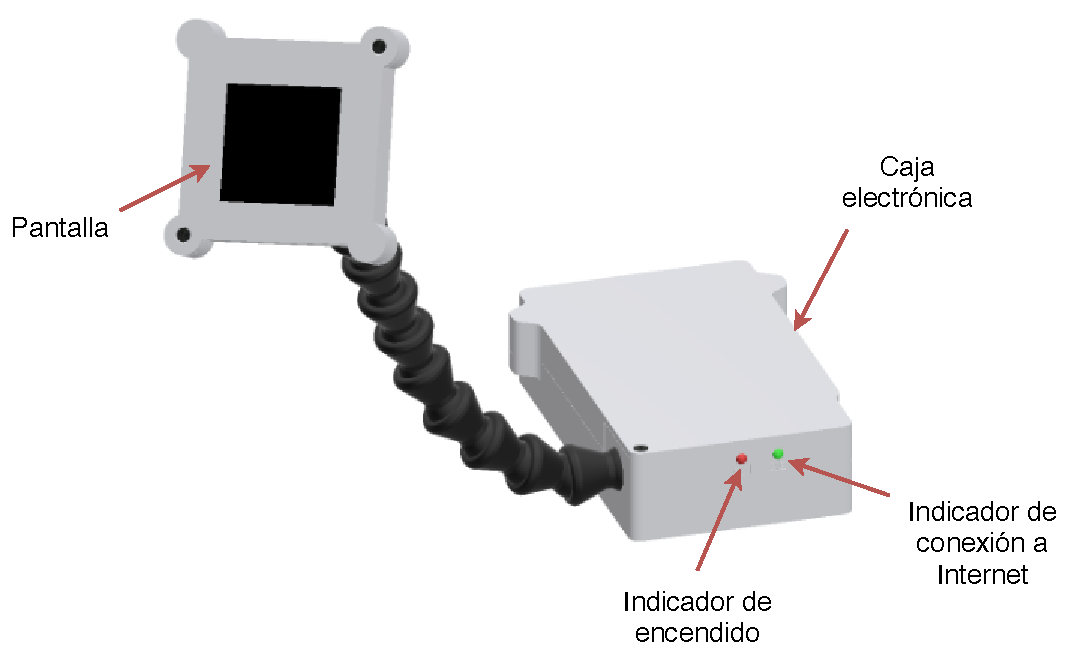
\includegraphics[width=\textwidth]{modelo_1.pdf}
\caption{Dispositivo de clasificación de estilo de conducción.}
\label{fig:modelo1}
\end{figure}

\begin{figure}[htbp!]
\centering
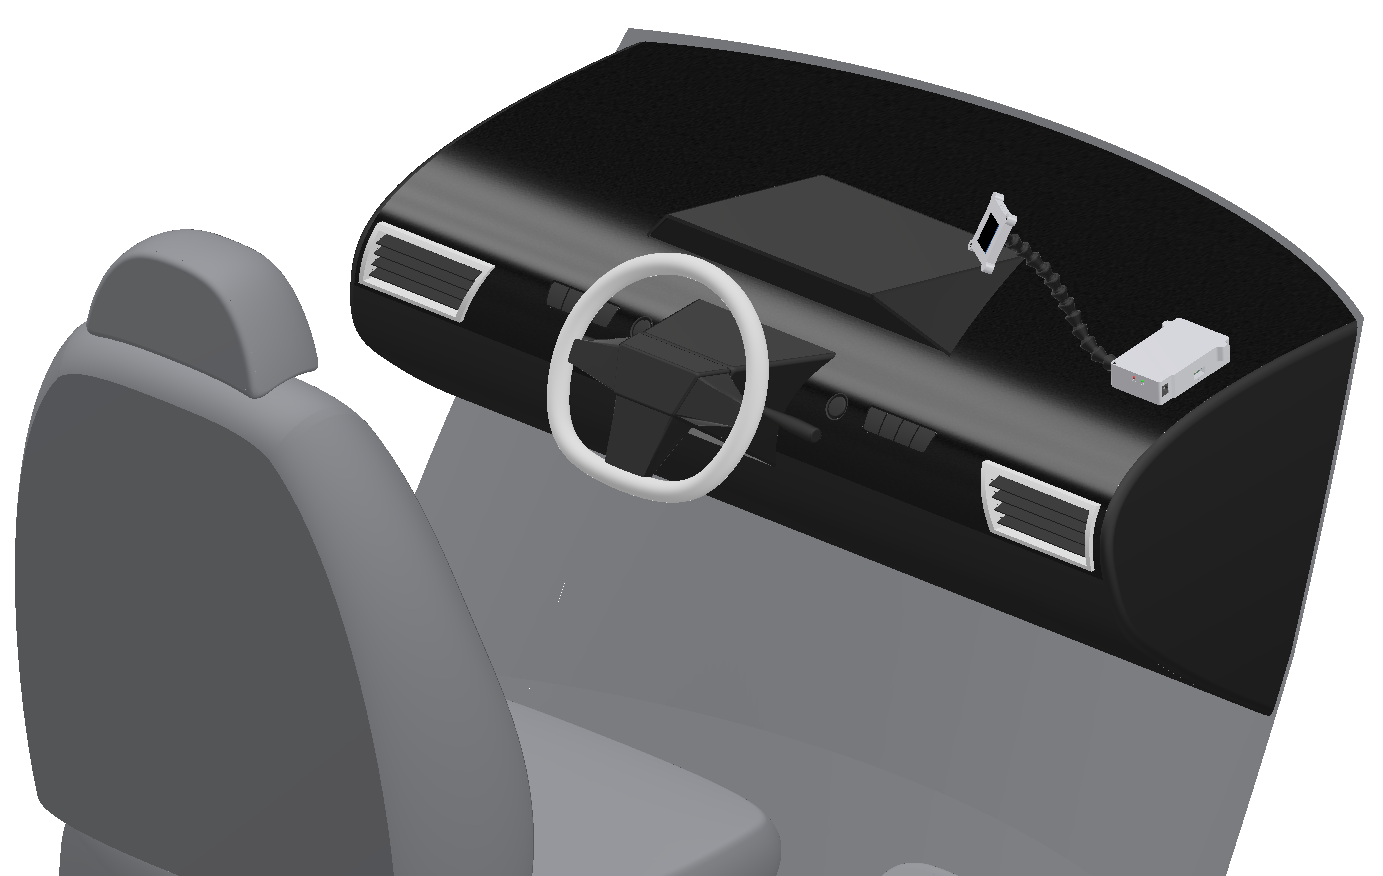
\includegraphics[width=\textwidth]{con_auto1.png}
\caption{Dispositivo de clasificación de estilo de conducción montado en un auto.}
\label{fig:modelo2}
\end{figure}

%Falta incluir otra figura de la vista superior con la tapa del case en transparencia
El sistema, Fig.~\ref{fig:modelo1} , esta compuesto por una placa electrónica que recogerá los datos de conducción usando sensores y estará contenida por una caja electrónica o case. Estos datos se enviarán a través de la red 2G a un servidor y este responderá con el estilo de conducción, el cual se mostrará en la pantalla.

Este dispositivo estará colocado en el panel frontal del vehículo como se puede apreciar en la Fig.~\ref{fig:modelo2}. Para sujetar el dispositivo al panel se usa cinta adhesiva de doble contacto. El dispositivo cuenta con 4 puertos: Puerto de carga, ranura de tarjeta Nano SIM y 2 puertos SMA para las antenas de GPS y GPRS/GSM.


\section{Funcionamiento del sistema mecatrónico}
Para comenzar, se deben verificar la conexión de alimentación al dispositivo y su conexión a Internet antes de iniciar el viaje del vehículo. Esto se puede comprobar observando las luces indicadora de 'Encendido' y 'Conexión'. El dispositivo cuenta con una ranura para una tarjeta Nano SIM y solo se conectará a Internet si existe una de estas tarjetas insertada en el dispositivo que cuente con un plan de datos activo.

Luego de verificar que las conexiones funcionan, se inicia el viaje del vehículo. El conductor debe ajustar la posición de la pantalla de tal manera de que la pueda visualizar sin ningún problema y que no bloquee la vista de este. El sistema empezará a recolectar datos del IMU, del GPS y de los sensores internos del vehículo a través del módulo OBD2 desde que el sistema se conecta a Internet por primera vez. De esta manera se registra el inicio de un nuevo viaje. Los datos recolectados por los sensores se graban en el microcontrolador, quién obtendrá la ubicación , velocidad y aceleración exacta del vehículo al combinar los datos del IMU y del GPS. Además calculará el consumo de combustible de los datos obtenidos a través del módulo OBD2. Luego enviará estos datos a la nube, en donde se guardarán en una base de datos y se ejecutará el algoritmo de clasificación. Al clasificar los datos se envían de regreso al dispositivo, quién se encargará de mostrar el resultado de la clasificación al conductor por medio de la pantalla.

La pantalla mostrará tan solo un símbolo con un color representativo para evitar distracciones del conductor. De esta manera el conductor podrá conocer si se encuentra manejando de una manera agresiva o no, con tan solo una mirada a la pantalla. Cada maniobra clasificada con un  estilo de conducción del conductor es registrada durante todo el viaje en la nube y se le otorga un puntaje de acuerdo a su nivel de agresividad. Mientras menos agresiva sea su puntaje será mayor. Se calculará luego un puntaje para toda la trayectoria realizada al sumar los puntajes de cada maniobra. Al final del día el conductor habrá realizado varias trayectorias y se calculará un promedio que se le asignará como indicador de desempeño.



\section{Diseño electrónico}
En esta sección se presentará primero el diagrama de bloques general del dispositivo. Luego se desarrollará la selección de cada componente y el diseño de las conexiones y de la placa electrónica.

\subsection{Diagrama de bloques}
En la Fig.~\ref{fig:bloques} se tiene el diagrama de bloques del dispositivo. El pre-procesamiento y la recolección de los datos de los sensores se llevará a cabo por medio de un ESP-WROOM-32. A este están conectados un IMU de 6 ejes (ICM-20648), por medio del protocolo I\textsuperscript{2}C; un módulo GPS (NEO-M8N), por medio de comunicación serial y una pantalla de tecnología IPS LCD (Con el controlador ST7789), por medio del protocolo SPI. El ESP-WROOM-32 enviará los datos pre-procesados por medio de un módulo GPRS/GSM (SIM800L), que se encuentra conectado a él por medio de comunicación serial. Por último el módulo OBD2 se encuentra conectado al puerto OBD2 del vehículo y se comunica inalámbricamente con el ESP-WROOM-32 usando comunicación serial a través de Bluetooth.

Todos estos elementos se alimentan usando la energía disponible del vehículo (\SI{12}{V} de la batería). El módulo OBD2 es el único elemento que se encuentra se parado del dispositivo principal y obtiene su energía a través del mismo puerto OBD2 por el cual esta conectado al vehículo. LOs demás componentes no pueden ser alimentados directamente con \SI{12}{V}, por lo que se necesita transformar el voltaje de acuerdo a los requerimientos de cada elemento. Esto se realiza en dos etapas, ya que se necesitan solo 2 voltajes distintos: \SI{4}{V} y \SI{3.3}{V}. La primera etapa de reducción se lleva a cabo por un regulador switching (TPS563210) que se encarga de regular el voltaje de \SI{12}{V} a \SI{4}{V} para alimentar al módulo GPRS/GSM (SIM800L). Luego se usa un regulador LDO (LT1764A) que se encarga de regular el voltaje de \SI{4}{V} a \SI{3.3}{V} que servirán para alimentar al microcontrolador, módulo GPS, IMU y a la pantalla.


\begin{figure}[htbp!]
\centering
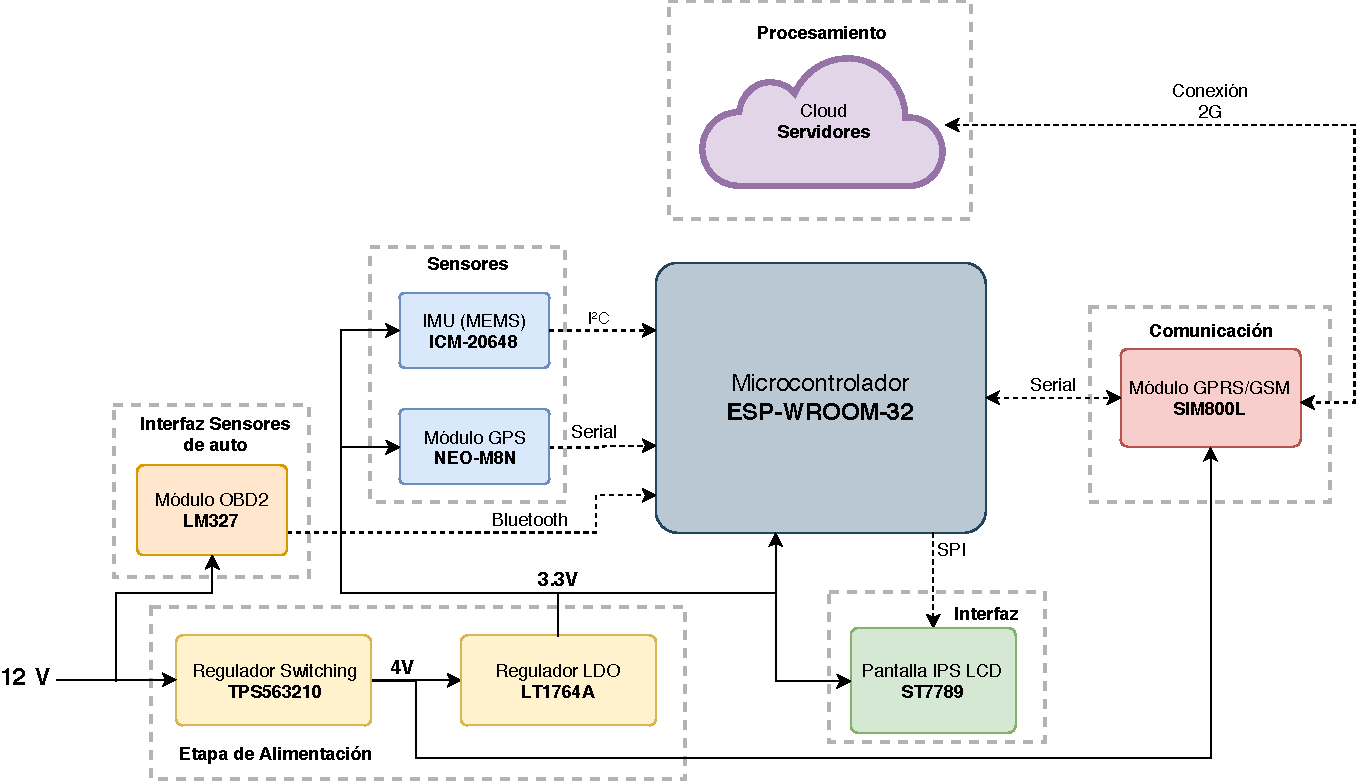
\includegraphics[width=\textwidth]{Bloques_principal.pdf}
\caption{Diagrama de bloques.}
\label{fig:bloques}
\end{figure}

\subsection{Componentes electrónicos}


\subsubsection{Inertial Measurement Unit (IMU)}
Este dispositivo cuenta con un acelerómetro, un giroscopio. Los datos registrados por estos sensores se pueden combinar para obtener el perfil de velocidad y aceleración, tanto longitudinal como lateral, del vehículo y estos perfiles aportan mucha información acerca del estilo de conducción del usuario.

Para seleccionar este componente empecemos por determinar las características que este debe poseer. En primer lugar el rango de medición debe ser el adecuado. En las investigaciones citadas  \cite{6957822}, \cite{constantinescu}, \cite{6083078},  \cite{Va-2013} La aceleración de los vehículos se suele encontrar dentro del rango de \SI{\pm7}{m/s^2}. Los rangos de medición de los acelerómetros se suelen expresar en \SI{}{g}, así que se necesita un acelerómetro que pueda medir en un rango de por lo menos \SI{\pm0.7}{g}

Realizando el mismo análisis para el giroscopio, en \cite{6083078} y \cite{6629603} se tiene que el rango mínimo de medición es de \SI{\pm57}{rad/s}

\bgroup
\def\arraystretch{1.5}%  1 is the default, change whatever you need
\begin{table}[htbp!]
\centering
\caption[Sensibilidad y Rango del ICM-20648]{Sensibilidad y Rango del ICM-20648 \cite{ICM20648}.}
\begin{tabular}{@{}P{3cm}P{3cm}P{3cm}P{3cm}@{}}
\toprule
Rango del Giroscopio (\si{\degree/sec}) & Sensibilidad del Giroscopio (\si{LSB/\degree/sec}) & Rango del Acelerómetro     (\si{g}) & Sensibilidad del Acelerómetro (\si{LSB/g}) \\ \midrule
\num{\pm 250} & 131 & \num{\pm 2} & 16384 \\
\num{\pm 500} & 65.5 & \num{\pm 4} & 8192 \\
\num{\pm 1000} & 32.8 & \num{\pm 8} & 4096 \\
\num{\pm 2000} & 16.4 & \num{\pm 16} & 2048 \\ \bottomrule
\end{tabular}
\label{diag:IMU1}
\end{table}

\egroup

El sensor que se eligió debido a que cumple con las características mencionadas anteriormente es el \textbf{ICM-20648} (Fig.~\ref{fig:IMU}) producido por TDK InvenSense. En las Tablas \ref{diag:IMU1} y \ref{diag:IMU2} se muestran sus principales características.


\bgroup
\def\arraystretch{1.5}%  1 is the default, change whatever you need
\begin{table}[htbp!]
\centering
\caption[Condiciones de Operación del ICM-20648]{Condiciones de Operación del ICM-20648 \cite{ICM20648}.}
\begin{tabular}{@{}ll@{}}
\toprule
Características & Valor \\ \midrule
Voltaje de alimentación & \SI{1.71}{V} - \SI{3.6}{V} \\
Corriente de operación & \SI{3.2}{mA} \\
Temperatura de operación & \SI{-40}{\celsius} hasta \SI{85}{\celsius} \\
Salida digital & I\textsuperscript{2}C o SPI \\
DMP & Onboard Digital Motion Processor \\ \bottomrule
\end{tabular}
\label{diag:IMU2}
\end{table}

\egroup

\begin{figure}[htb!]
\centering
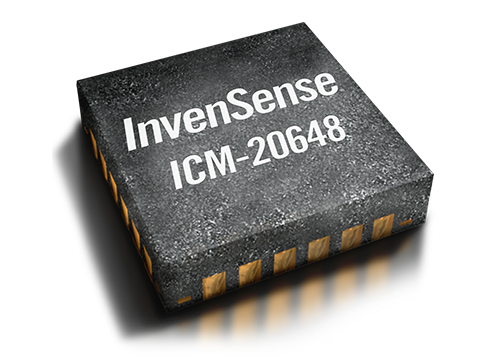
\includegraphics[width=0.4\textwidth]{ICM-20648.png}
\caption{ICM-20648, IMU de 6 grados de libertad.}
\label{fig:IMU}
\end{figure}

\newpage

\subsubsection{Módulo GPS}
Este módulo se encargará de detectar la posición exacta del vehículo en coordenadas. Para hacer esto se puede recurrir a distintos servicios del Sistema mundial de navegación por satélite (GNSS). Actualmente se encuentran dos operativos completamente: GPS y GLONASS. Es primero es el servicio hecho por Estados Unidos y el segundo es el realizado por Rusia. Es importante considerar la capacidad de los diferentes módulos para poder acceder a estos dos servicios.

Las características que debe tener el módulo de GPS son las siguientes:
\begin{itemize}
    \itemsep0em
    \item Bajo consumo.
    \item Poder acceder tanto a GPS como a GLONASS.
    \item Por lo menos una frecuencia de muestreo de \SI{1}{Hz}.
\end{itemize}

El modulo de GPS que cumple con estas características es el \textbf{NEO-M8N} de Ublox (Fig.~\ref{fig:GPS}). En la Tabla~\ref{diag:GPS} se resumen sus principales características.
\begin{figure}[hbtp!]
\centering
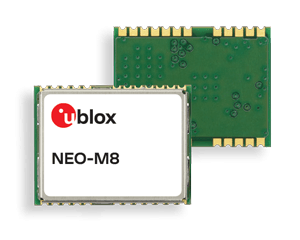
\includegraphics[width=0.5\textwidth]{NEO-M8.png}
\caption[NEO-M8N, módulo GPS]{NEO-M8N, módulo GPS \cite{GPS}.}
\label{fig:GPS}
\end{figure}

\bgroup
\def\arraystretch{1.5}%  1 is the default, change whatever you need
\begin{table}[htbp!]
\centering
\caption[Características del NEO-M8N]{Características del NEO-M8N \cite{GPS}.}
\begin{tabular}{@{}ll@{}}
\toprule
Características & Valor \\ \midrule
GNSS & GPS, GLONASS, GALIEO y BeiDou \\
Precisión & \SI{2.5}{m} \\
Frecuencia máxima & \SI{5}{Hz} \\
Protocolos de Comunicación & UART, I\textsuperscript{2}C, SPI \\
Voltaje de operación & \SI{2.7}{V} - \SI{3.6}{V} \\
Corriente de operación & \SI{32}{mA} \\
Corriente máxima & \SI{67}{mA} \\
Temperatura de Operación & \SI{-40}{\celsius} hasta \SI{85}{\celsius} \\\bottomrule
\end{tabular}
\label{diag:GPS}
\end{table}
\egroup






\subsubsection{Módulo GPRS/GSM}
El módulo GPRS/GSM es capaz de conectarse a las red 2G. Esta red es la que tiene mayor cobertura en el Perú (Fig.~\ref{fig:Cobertura}) ya que es la más antigua. Esta red puede alcanzar hasta una velocidad de \SI{114}{kbps} y es la de menor consumo energético, comparada con 3G y 4G. Usando este módulo se enviarán los datos recopilados por el sistema a través de Internet y se asegurará su conexión en todo momento.

\begin{figure}[hbtp!]
\centering
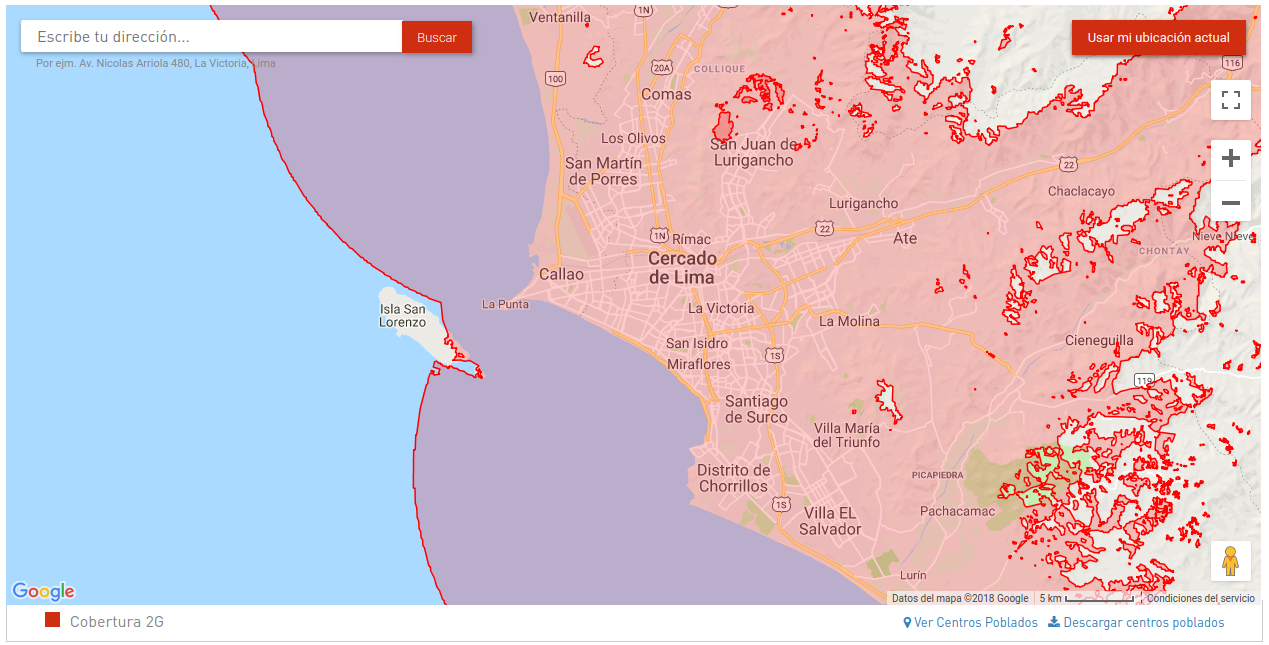
\includegraphics[width=\textwidth]{Cobertura_2G.png}
\caption[Cobertura de la red 2G de Claro]{Cobertura de la red 2G de Claro \cite{Cobertura_claro}.}
\label{fig:Cobertura}
\end{figure}

Una opción muy popular es el módulo \textbf{SIM 800L} (Fig.~\ref{fig:SIM}) que debido a sus características, expuestas en la Tabla~\ref{diag:SIM}, su disponibilidad y su bajo precio lo hacen adecuado para ser usado en este sistema.

\begin{figure}[hbtp!]
\centering
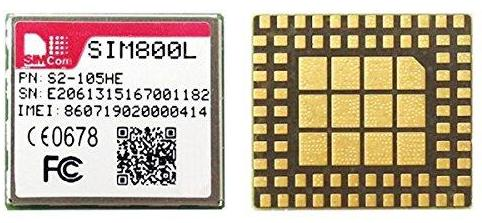
\includegraphics[width=0.6\textwidth]{SIM800L.jpg}
\caption[SIM 800L, módulo GPRS/GSM]{SIM 800L, módulo GPRS/GSM \cite{SIM800L}.}
\label{fig:SIM}
\end{figure}

\bgroup
\def\arraystretch{1.5}%  1 is the default, change whatever you need
\begin{table}[htbp!]
\centering
\caption[Características del SIM 800L]{Características del SIM 800L \cite{SIM800L}.}
\begin{tabular}{@{}p{5.4cm}p{8cm}@{}}
\toprule
Características & Valor \\ \midrule
Voltaje de operación & \SI{3.4}{V} -  \SI{4.4}{V} \\
Corriente promedio en Reposo & \SI{18.7}{mA} \\
Corriente promedio durante \mbox{transmisión} & \SI{453.57}{mA} \\
Corriente máxima & \SI{2}{A} (Solo durante ráfaga de transmisión) \\
Temperatura de operación & \SI{-40}{\celsius} hasta \SI{85}{\celsius} \\
Velocidad de transmisión & máx. \SI{85.6}{kbps} \\
Bandas de frecuancia & Quad-band: GSM 850, EGSM 900, DCS 1800, PCS 1900 \\ \bottomrule
\end{tabular}
\label{diag:SIM}
\end{table}
\egroup






\subsubsection{Pantalla}
La pantalla cumplirá el rol de mostrar la clasificación del estilo de conducción del usuario. Para poder transmitir la información sin generar distracciones se usarán símbolos y colores para representar los estilos de conducción.

Además se necesita que la pantalla se pueda observar bien tanto a la luz del día, por lo que su ángulo de visibilidad y su brillo serán factores importantes también.

Por último, el tamaño de la pantalla debe permitir la identificación del símbolo por parte del conductor. Basados en estos parámetros se puede elegir entre usar 3 tecnologías muy populares: LCD, OLED e IPS LCD.

Las pantallas LCD pueden alcanzar una densidad de imagen más alta que las OLED. Sin embargo, las OLED tienen un mejor ángulo de visión y un menor consumo. Por otro lado, las IPS LCD tienen también un muy buen ángulo de visión y buena densidad de imagen.

\bgroup
\def\arraystretch{1.5}%  1 is the default, change whatever you need
\begin{table}[htb!]
\centering
\caption{Alternativas de pantallas}
\begin{tabular}{@{}p{1.6cm}lllP{3cm}lc@{}}
\toprule
Nr. \mbox{Producto} & Tecnología & Controlador & Tamaño & Voltaje de Operación & Precio & Resolución\\ \midrule
1431 & OLED & SSD1351 & \SI{1.5}{in} & \SI{3.3}{V} o \SI{5}{V} & \textdollar \num{39.95} & 128x128\\
2088 & LCD & ST7735R & \SI{1.44}{in} & \SI{3.3}{V} o \SI{5}{V} & \textdollar \num{14.95} & 128x128\\
3787 & IPS LCD & ST7789 & \SI{1.54}{in} & \SI{3.3}{V} o \SI{5}{V} & \textdollar \num{19.95} & 240x240\\ \bottomrule
\end{tabular}
\label{diag:Display}
\end{table}
\egroup

En la Tabla.~\ref{diag:Display} se pueden ver 3 alternativas para la pantalla. De estas se escoge la pantalla IPS LCD (Fig.~\ref{fig:Display}), ya que tiene buen ángulo de visibilidad, tamaño y resolución.


\begin{figure}[hbt!]
\centering
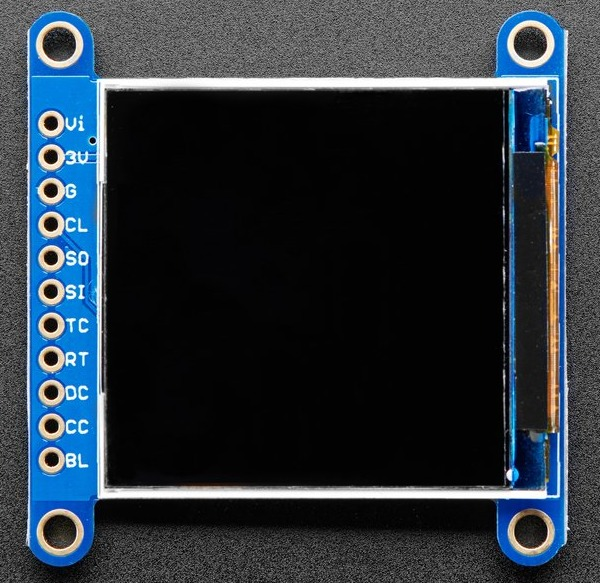
\includegraphics[width=0.8\textwidth]{IPS_LCD.jpg}
\caption[Adafruit 1.54" 240x240 Wide Angle TFT LCD Display - ST7789]{Adafruit 1.54" 240x240 Wide Angle TFT LCD Display - ST7789 \cite{IPS_LCD}.}
\label{fig:Display}
\end{figure}











\subsubsection{Módulo OBD2}
Este módulo se encargará de acceder a todos los parámetros internos del auto conectándose directamente a las ECU \textit{(Electronic Control Units)} del motor. Para poder leer estos parámetros diversas marcas de autos usan distintos protocolos de comunicación. En la Tabla~\ref{diag:OBD} Se muestran distintos protocolos y en cada columna circuitos integrados ELMXXX que se usan para comunicarse con el puerto OBD2.

\bgroup
\def\arraystretch{1.5}%  1 is the default, change whatever you need
\begin{table}[htbp!]
\centering
\caption[Protocolos y Circuitos integrados]{Protocolos y Circuitos integrados \cite{OBD}.}
\begin{tabular}{|l|P{1.5cm}|P{1.5cm}|P{1.5cm}|P{1.5cm}|P{1.8cm}|}
\hline
 &  ELM323 & ELM325 & ELM327  & ELM329 & ELM329L \\ \hline
SAE J1850-PWM   &  &  & \si{\surd}  &  &  \\ \hline
SAE J1850-VPW   &  &  & \si{\surd}  &  &  \\ \hline
ISO 9141-2   & \si{\surd} &  & \si{\surd}  &  &  \\ \hline
ISO 14230-4 (slow)     & \si{\surd} &  & \si{\surd}  &  &  \\ \hline
ISO 14230-4 (fast)     & \si{\surd} &  & \si{\surd} &  \si{\surd} & \si{\surd} \\ \hline
ISO 15765-4 (CAN)     &  &  & \si{\surd} & \si{\surd} &  \si{\surd} \\ \hline
SAE J1939 (250kbps)     &  &  & \si{\surd} & \si{\surd} &  \si{\surd} \\ \hline
SAE J1939 (500kbps)     &  &  & \si{\surd} & \si{\surd} & \si{\surd} \\ \hline
SAE J1708 (J1587)     &  & \si{\surd} &  &    &  \\ \hline
SAE J1708 (J1922)     &  & \si{\surd} &  &    &  \\ \hline
\end{tabular}
\label{diag:OBD}
\end{table}
\egroup

Para maximizar la compatibilidad con vehículos se escoge el modulo \textbf{ELM327}. Este IC convierte los protocolos mencionados a comunicación serial y puede transmitir los datos a través de un cable, WiFi o Bluetooth. Para esta aplicación se escoge la versión que usa Bluetooth (Fig.~\ref{fig:OBD}) ya que el conector se encontrará a menos de \SI{2}{m} del conector, permitiéndole usar esta tecnología que consume menos energía que el WiFi y es inalámbrica también.

\begin{figure}[hbtp!]
\centering
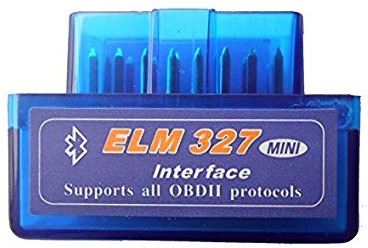
\includegraphics[width=0.35\textwidth]{OBD.jpg}
\caption[ELM327 - OBD2 interface]{ELM327 - OBD2 interface \cite{OBD}.}
\label{fig:OBD}
\end{figure}








\subsubsection{Microcontrolador}
El microcontrolador a seleccionar necesita poder comunicarse con todos los módulos anteriores, poder manejar protocolos como MQTT y CoAP y además realizar procesamiento básico de fusión de sensores (mezclar los datos obtenidos del IMU y del GPS). Se ha escogido para este sistema al ESP-WROOM-32 (Fig.~\ref{fig:esp-wroom32})

Este microcontrolador cuenta con el diagrama de bloques expuesto en la Fig.~\ref{fig:Bloques_esp32} y como se puede apreciar, cuenta con I\textsuperscript{2}C para comunicarse con el IMU, UART para comunicarse con el módulo GPS y el módulo GPRS/GSM, SPI para controlar la pantalla y Bluetooth para comunicarse con el módulo OBD2. Además presenta la suficiente potencia para realizar las tareas anteriormente descritas. Un resumen de sus características se encuentra en la Tabla~\ref{diag:ESP32}.

\begin{figure}[hbtp!]
\centering
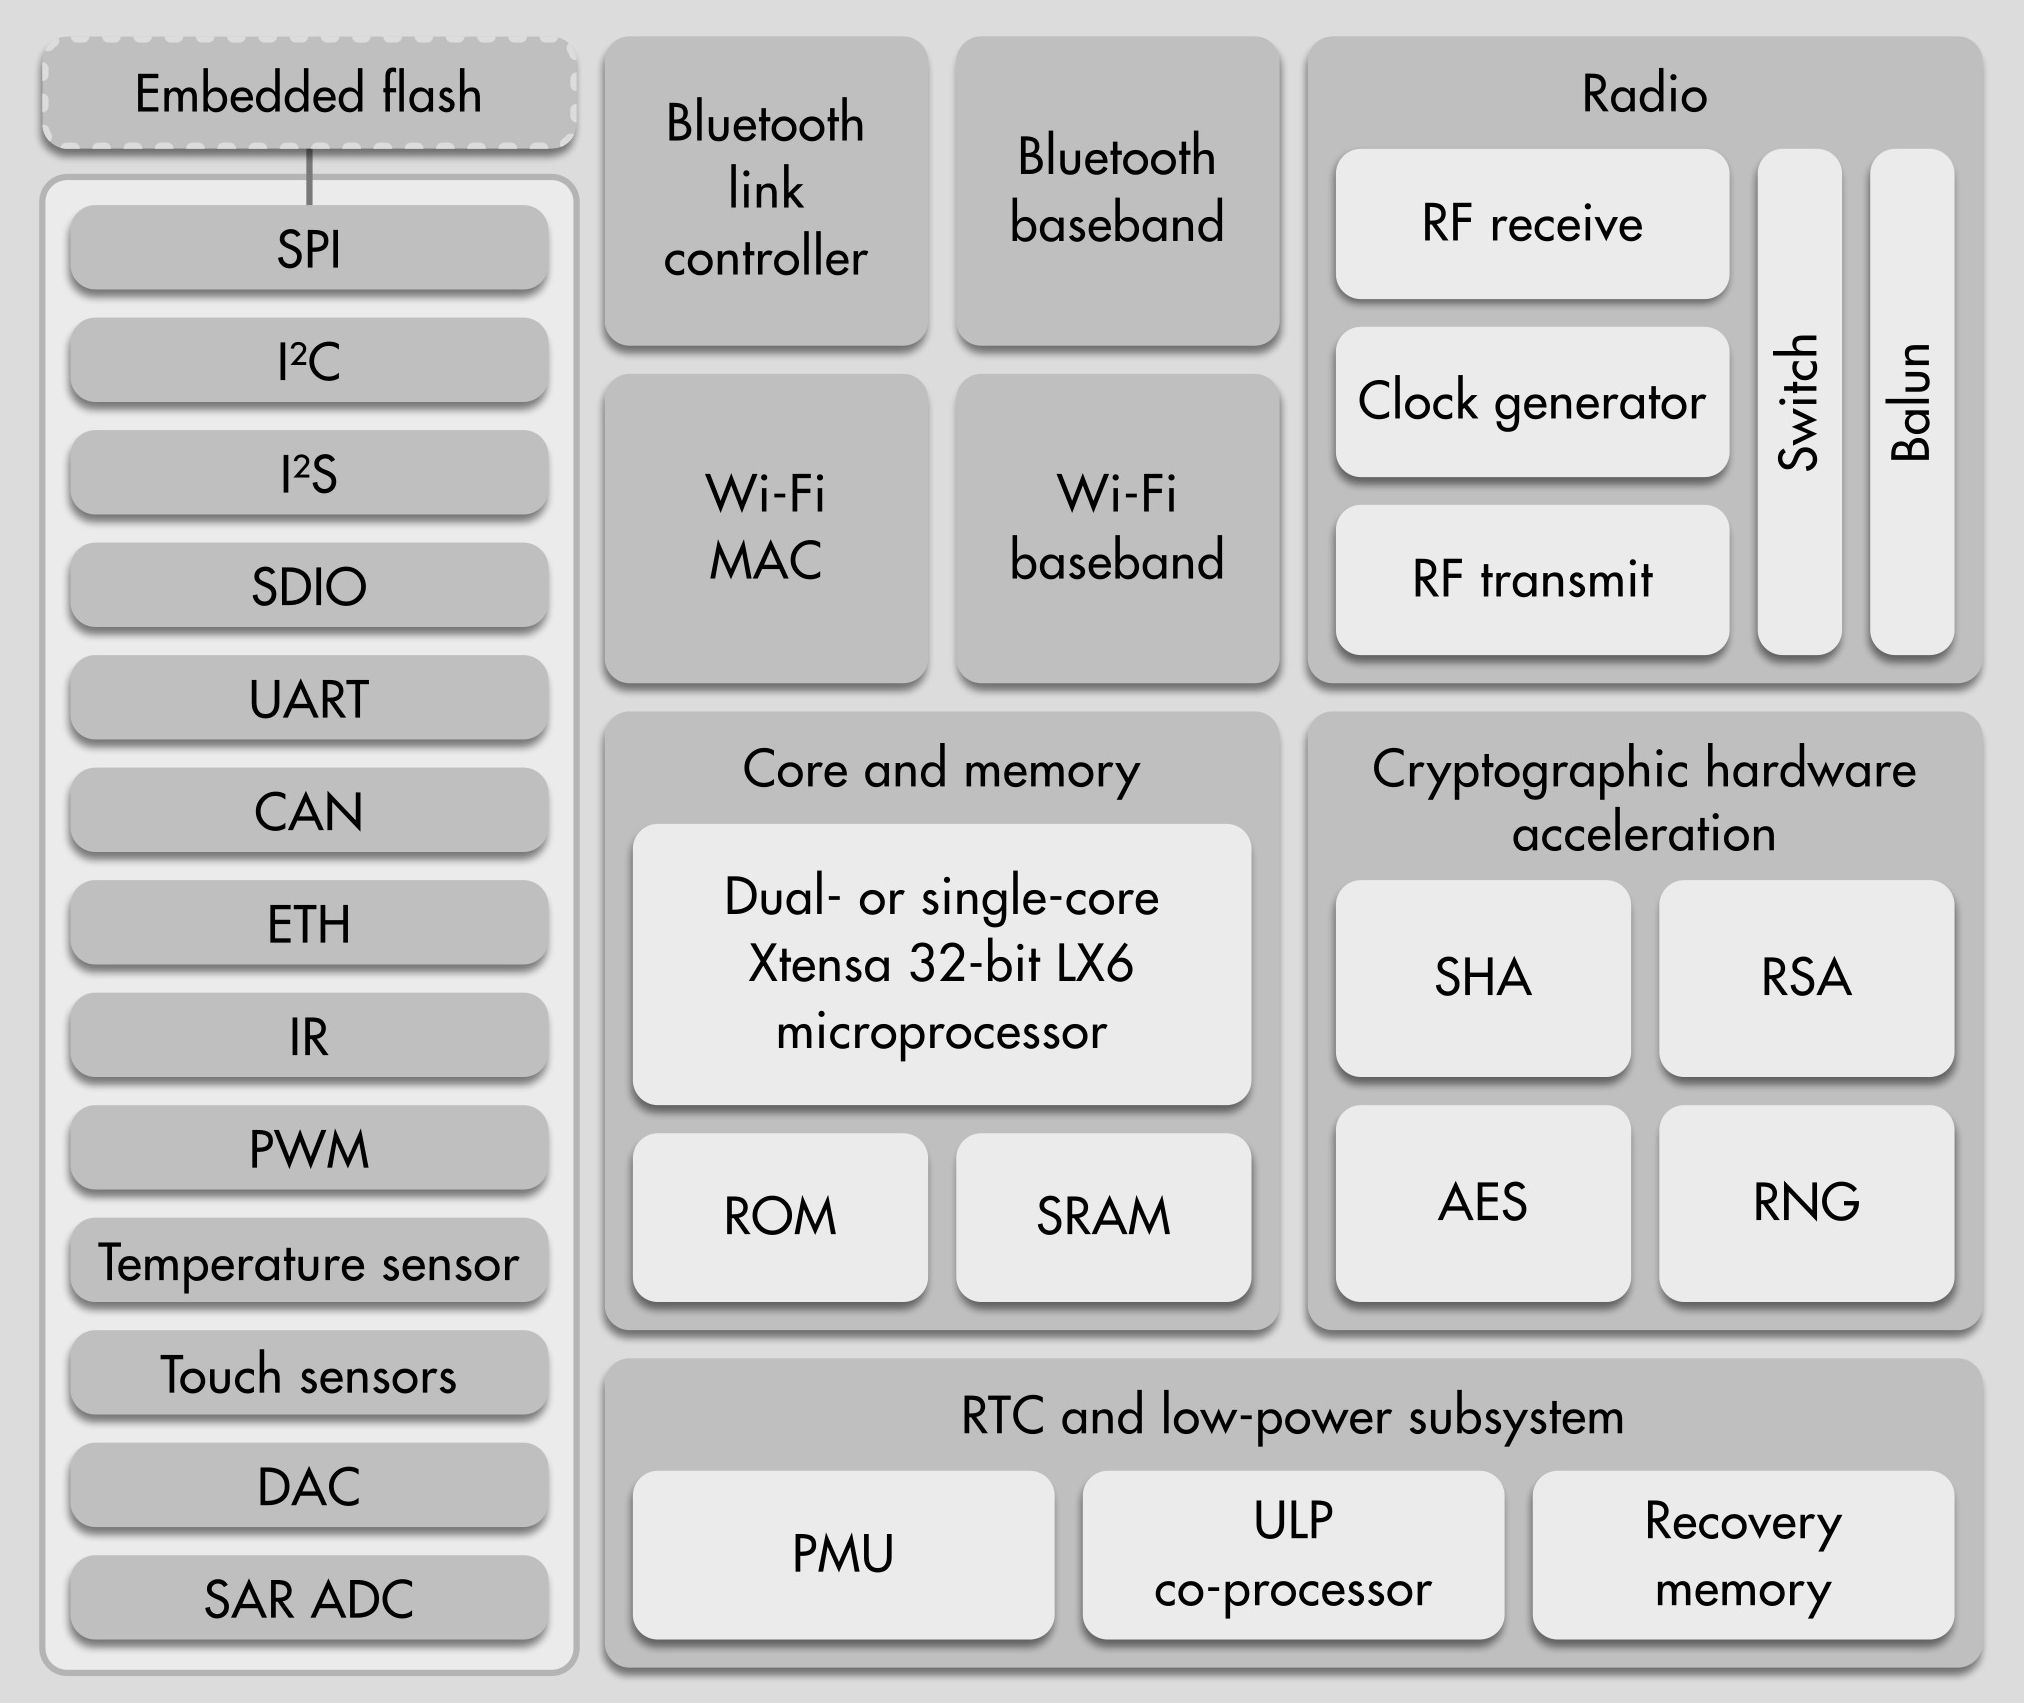
\includegraphics[width=0.9\textwidth]{ESP32_Function_Block_Diagram.jpg}
\caption{Diagrama de Bloques del ESP32  \cite{Esp32}.}
\label{fig:Bloques_esp32}
\end{figure}


\begin{figure}[hbtp!]
\centering
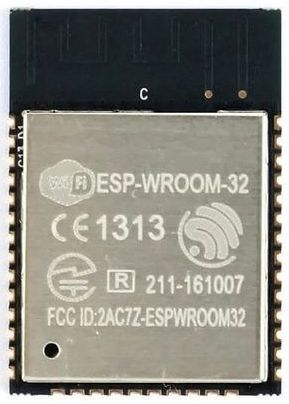
\includegraphics[width=0.3\textwidth]{esp32.jpg}
\caption{ESP-WROOM-32 \cite{ESP32_page}.}
\label{fig:esp-wroom32}
\end{figure}

\bgroup
\def\arraystretch{1.5}%  1 is the default, change whatever you need
\begin{table}[htbp!]
\centering
\caption[Características del ESP-WROOM-32]{Características del ESP-WROOM-32 \cite{Esp32_Hardware}.}
\begin{tabular}{@{}lp{9cm}@{}}
\toprule
Características & Valor \\ \midrule
Voltaje de Operación & \SI{2.7}{V} - \SI{3.6}{V} \\
Corriente máxima & \SI{500}{mA} \\
Corriente de operación & \SI{80}{mA} \\
Corriente en sleep mode & \SI{5}{\uA} \\
Frecuencia del CPU & \SI{240}{MHz} \\
Temperatura de operación & \SI{-40}{\celsius} hasta \SI{85}{\celsius} \\
Interfaces & SD card, UART, SPI, SDIO, I\textsuperscript{2}C, LED PWM, Motor PWM, I 2 S,IR, contador de pulsos, GPIO, sensor táctil capacitivo, ADC, DAC \\
Connectividad & WiFi (802.11 b/g/n (802.11n up to 150 Mbps) Bluetooth (Bluetooth v4.2 BR/EDR y BLE)\\\bottomrule
\end{tabular}
\label{diag:ESP32}
\end{table}
\egroup









\subsubsection{Regulador switching}
Una vez escogidos los componentes a usar en las secciones anteriores, se calculará el consumo total de los componentes para poder diseñar la etapa de alimentación del sistema. En la Tabla~\ref{diag:consumo} se encuentra un resumen de cada dispositivo con su voltaje de operación y su corriente máxima de consumo.

\bgroup
\def\arraystretch{1.5}%  1 is the default, change whatever you need
\begin{table}[htbp!]
\centering
\caption[Consumo de los componentes del sistema]{Consumo de los componentes del sistema.}
\begin{tabular}{@{}lp{2cm}p{2cm}p{2cm}@{}}
\toprule
Dispositivo & Voltaje de Operación & Corriente máxima & Potencia máxima\\ \midrule
IMU (ICM-20648) & \SI{3.3}{V} & \SI{3.2}{\mA} & \SI{10.56}{\mW} \\
Módulo GPS (NEO-M8N) & \SI{3.3}{V} & \SI{67}{mA} & \SI{221,1}{\mW}\\
Módulo GPRS/GSM (SIM800L) & \SI{4}{V} & \SI{2000}{mA} & \SI{8000}{\mW}\\
Pantalla IPS LCD & \SI{3.3}{V} & \SI{50}{mA} & \SI{165}{\mW}\\
OBD2 (ELM237) & \SI{5}{V} & \SI{12}{mA} & \SI{60}{\mW}\\
ESP-WROOM-32 & \SI{3.3}{V} & \SI{500}{mA} & \SI{1650}{\mW}\\ \bottomrule
\end{tabular}
\label{diag:consumo}
\end{table}
\egroup

Sin embargo, El módulo OBD2 (ELM237) no estará conectado junto con los demás componentes. Este módulo se conectará al puerto OBD2 del Auto y obtendrá energía de esta misma conexión sin necesidad de diseñarle un regulador de voltaje.


Si sumamos la potencia máxima de cada dispositivo, obtendremos la potencia mínima necesaria que se debe poder entregar por el regulador de voltaje. Esta suma da como resultado \textbf{10.046 W}.


\begin{figure}[hbtp!]
\centering
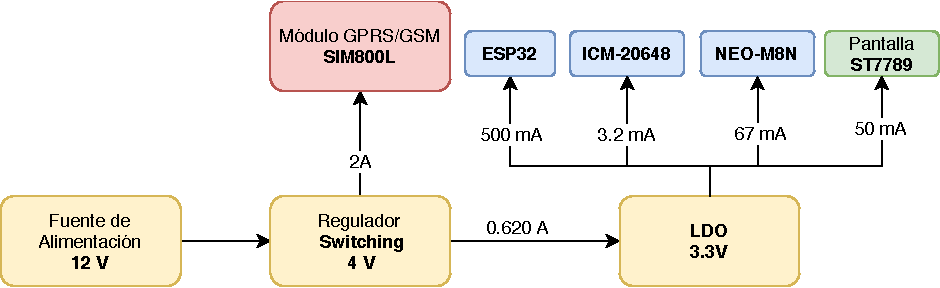
\includegraphics[width=\textwidth]{Bloques_Alimentacion.pdf}
\captionsetup{justification=centering,margin=2cm}
\caption{Diagrama de bloques de las etapas de alimentación con la corriente máxima de cada dispositivo.}
\label{fig:bloques_alim}
\end{figure}



Se propone dos etapas de regulación de voltaje debido a que se necesitan 2 niveles de voltaje, \SI{4}{V} y \SI{3.3}{V}. En la primera etapa se usará un regulador switching para obtener \SI{4}{V} de los \SI{12}{V} disponibles en la alimentación. Y en la segunda etapa se usará un LDO (Low Dropout Regulator) para obtener los \SI{3.3}{V} a partir de los \SI{4}{V}. En la Fig.~\ref{fig:bloques_alim} se dispone de manera gráfica e ideal la potencia y las corrientes máximas que deben poder entregar los reguladores de voltaje.



Entonces usando  la Fig.~\ref{fig:bloques_alim} Se tiene que el regulador switching debe poder entregar por lo menos \SI{2.62}{A}. Se selecciona el circuito integrado \textbf{TPS563210} que tiene las características mencionadas en la Tabla~\ref{diag:Switching}

\bgroup
\def\arraystretch{1.5}%  1 is the default, change whatever you need
\begin{table}[htbp!]
\centering
\caption[Características del TPS563210]{Características del TPS563210 \cite{TPS563210}.}
\begin{tabular}{@{}ll@{}}
\toprule
Características & Valor \\ \midrule
Voltaje de entrada & \SI{4.5}{V} - \SI{17}{V} \\
Voltaje de salida & \SI{0.76}{V} - \SI{7}{V} \\
Corriente máxima de operación & \SI{3}{A} \\
Frecuencia de conmutación & \SI{650}{kHz} \\
Temperatura de operación de la juntura & \SI{-40}{\celsius} - \SI{150}{\celsius}\\
Resitencia térmica de juntura-ambiente & \SI{87}{\celsius/W}\\\bottomrule
\end{tabular}
\label{diag:Switching}
\end{table}
\egroup


Se calcula entonces si este regulador switching es capaz de entregar \SI{2.62}{A} o \SI{10.046}{W} sin usar un disipador. Para esto se usa la Ecuación~\ref{eq:disipadores}
\begin{equation}
   T_J=T_A+(R_{\theta JA} \times Potencia_{dis})
   \label{eq:disipadores}
\end{equation}

La $Potencia_{dis}$ en esta ecuación es la potencia disipada la cual se puede calcular a partir de la eficiencia del regulador. Según el datasheet \cite{TPS563210}, se tiene una eficiencia del 93\% cuando el voltaje de salida es \SI{4}{V} y la corriente de salida es \SI{2.6}{A}.
\begin{equation}
    Potencia_{dis}=\frac{Potencia_{salida}}{Eficiencia}\times(1-Eficiencia)
     \label{eq:potencia}
\end{equation}
Usando la Ecuación.~\ref{eq:potencia} se obtiene que el regulador disipará:
 $$Potencia_{dis}=\SI{0.75}{W}$$

Al usar $T_A=\SI{25}{\celsius}$,  $R_{\theta JA}=\SI{87}{\celsius/W}$ y $Potencia_{dis}=\SI{0.75}{W}$ en  la Ecuación~\ref{eq:disipadores} resulta:
$$T_J=\SI{90.25}{\celsius}$$
Esto significa que el regulador podrá operar sin necesidad de usar un disipador para esta aplicación ya que el máximo para $T_J$ es \SI{150}{\celsius}


\subsubsection{Regulador LDO}


Ahora es momento de elegir el regulador LDO. Para esta etapa se usará el IC \textbf{LT1764A} que posee las características mencionadas en la Tabla~\ref{diag:LDO}.

\bgroup
\def\arraystretch{1.5}%  1 is the default, change whatever you need
\begin{table}[htbp!]
\centering
\caption[Características del LT1764A]{Características del LT1764A \cite{LT1764A}.}
\begin{tabular}{@{}ll@{}}
\toprule
Características & Valor \\ \midrule
Voltaje de entrada & \SI{2.7}{V} - \SI{20}{V} \\
Voltaje de salida & \SI{3.3}{V} \\
Corriente máxima de operación & \SI{3}{A} \\
Dropout Voltage & \SI{340}{mV} a \SI{3}{A} \\
Temperatura de operación de la juntura & \SI{-40}{\celsius} - \SI{150}{\celsius}\\
Resitencia térmica de juntura-ambiente & \SI{30}{\celsius/W}\\\bottomrule
\end{tabular}
\label{diag:LDO}
\end{table}
\egroup



Se comenzará por realizar el análisis térmico de este integrado. La potencia disipada se calcula usando la Ecuación~\ref{eq:pot_LDO}.
\begin{equation}
    Potencia_{dis}=I_{OUT(MAX)}\times(V_{IN(MAX)}-V_{OUT})+I_{GND}\times V_{IN(MAX)} \label{eq:pot_LDO}
\end{equation}
Se reemplazan los siguientes valores en esta ecuación:
\begin{align*}
    V_{OUT}&=\SI{3.3}{V}&
    V_{IN(MAX)}&=\SI{4}{V}&
    I_{OUT(MAX)}&=\SI{0.62}{A}&
    I_{GND}&=\SI{20}{mA}&
\end{align*}
Y se obtiene el siguiente resultado:
$$ Potencia_{dis}=\SI{0.514}{W}$$

Ahora se aplica la Ecuación~\ref{eq:disipadores} con la que obtendremos la Temperatura de la juntura ($T_J$) que se alcanzará al disipar esa potencia.
$$ T_J=\SI{40.42}{\celsius}$$
Como la $T_{J(MAX)}=\SI{150}{\celsius}$, se puede afirmar que no se necesita disipador para usar este regulador. Con el sistema de alimentación definido se puede graficar el diagrama de bloques completo del sistema (Fig.~\ref{fig:Bloques_comp}). En esta ocasión se colocaron los valores promedio de corriente que consumirá cada dispositivo. Observando este diagrama se puede obtener la potencia promedio que consumirá el dispositivo $P_{prom}=\SI{2.66}{W}$.

\begin{figure}[hbtp!]
\centering
\makebox[\textwidth][c]{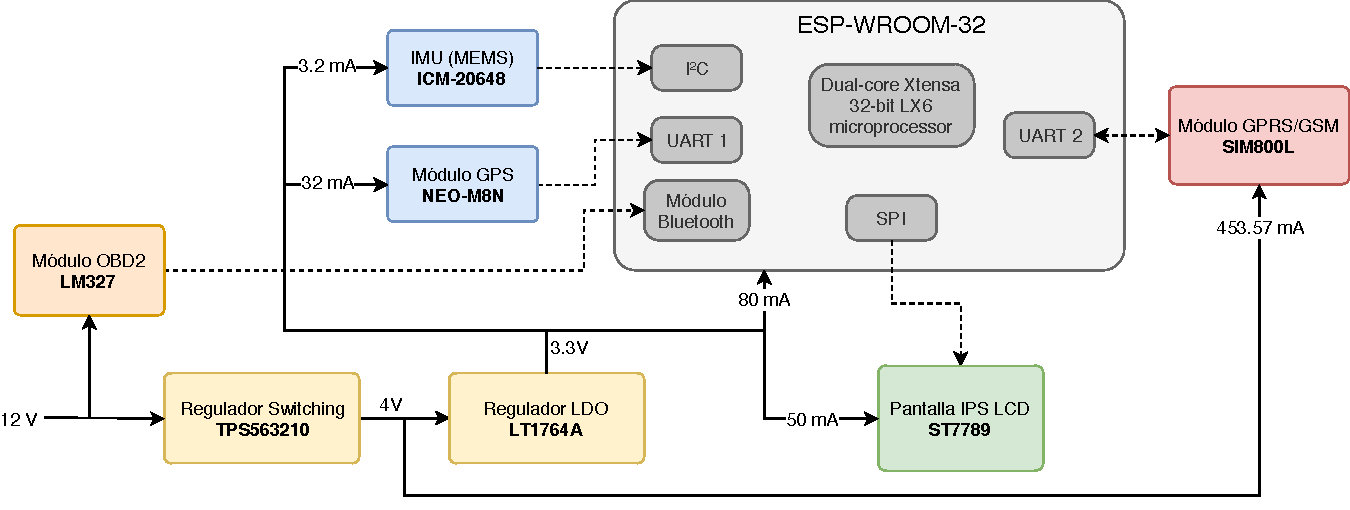
\includegraphics[width=\textwidth]{Bloques_total.pdf}}%
\caption{Diagrama de bloques del sistema con corrientes promedio.}
\label{fig:Bloques_comp}
\end{figure}



\subsection{Diagramas electrónicos}
En esta sección se presentarán las conexiones de los componente seleccionados anteriormente. Estas conexiones se realizaron siguiendo las recomendaciones que se encuentran en las hojas de datos de cada componente.

\subsubsection{IMU}
Se realiza el esquemático (Fig.~\ref{fig:IMU_esquem}) mostrando las conexiones necesarias para poder alimentar al módulo y para que este pueda comunicarse con el microcontrolador. Se establece el voltaje de alimentación y el voltaje lógico a \SI{3.3}{V}. En la hoja de datos \cite{ICM20648} se recomiendan los valores de los capacitores y se conectan los pines necesarios para poder implementar el protocolo de comunicación I\textsuperscript{2}C. El pin 9 se conecta a GND para establecer la dirección I\textsuperscript{2}C a b1101000.

\begin{figure}[htb!]
\centering
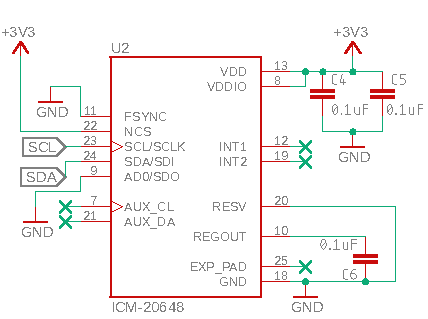
\includegraphics[width=\textwidth]{IMU_esquem.pdf}
\caption{Esquemático del módulo ICM-20648.}
\label{fig:IMU_esquem}
\end{figure}




\subsubsection{Módulo GPS}
Se realiza el esquemático (Fig.~\ref{fig:GPS_esquem}) de las conexiones necesarias para alimentar al módulo e implementar la comunicación con el microcontrolador. En este caso se alimenta al módulo con \SI{3.3}{V} y se implementa comunicación serial con el microcontrolador. Además se tiene un conector SMA para poder conectar una antena externa y también se cuenta con una batería de \SI{3}{V}, con una capacidad de \SI{5}{mAh} según \cite{MS621FE}.

Esta batería, que se recomienda en la hoja de datos \cite{GPS}, se encargará de mantener activo al módulo GPS en modo de bajo consumo durante la noche cuando la fuente de voltaje principal este desconectada. Esto se quiere hacer debido a que el GPS encontrará la posición de una forma más rápida si se mantiene activo. En cambio, cuando se apaga y se vuelve a encender se le llama "encendido en frío" y toma más tiempo.

\begin{figure}[htbp!]
\centering
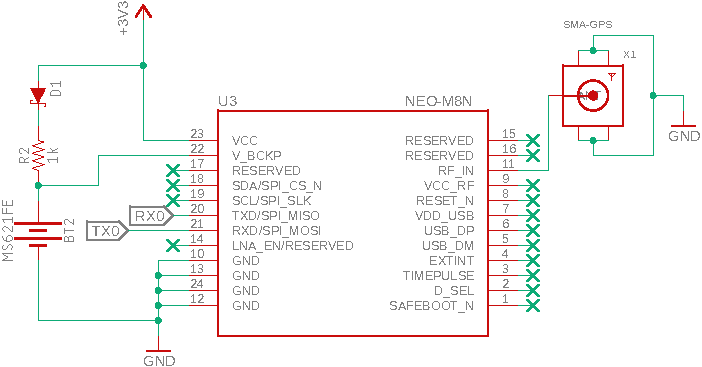
\includegraphics[width=\textwidth]{GPS_esquem.pdf}
\caption{Esquemático del módulo NEO-M8N.}
\label{fig:GPS_esquem}
\end{figure}



\subsubsection{Módulo GPRS/GSM}
A partir de los parámetros mencionados en la Tabla~\ref{diag:SIM} y de la hoja de datos \cite{SIM800L} se realiza el esquemático (Fig.~\ref{fig:GSM_esquem}) de las conexiones necesarias para alimentar al módulo e implementar la comunicación con el microcontrolador.

\begin{figure}[htb!]
\centering
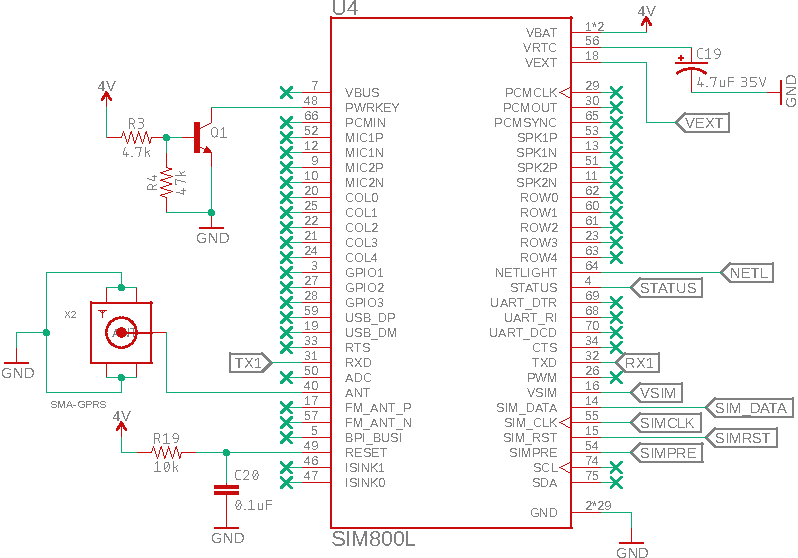
\includegraphics[width=\textwidth]{GSM_esquem.pdf}
\caption{Esquemático del módulo SIM800L.}
\label{fig:GSM_esquem}
\end{figure}

En este caso el módulo es alimentado con \SI{4}{V} y se usará comunicación serial. Los capacitores elegidos son recomendaciones de la hoja de datos \cite{SIM800L} al igual que el transistor que cumplirá la función de encender y apagar correctamente el módulo.

Además se necesita de un módulo que lea una tarjeta SIM. En la Fig.~\ref{fig:GSM_SIM_esquem} se muestra el esquemático de este módulo, el lector de tarjetas SIM (SIM8055).

\begin{figure}[htbp!]
\centering
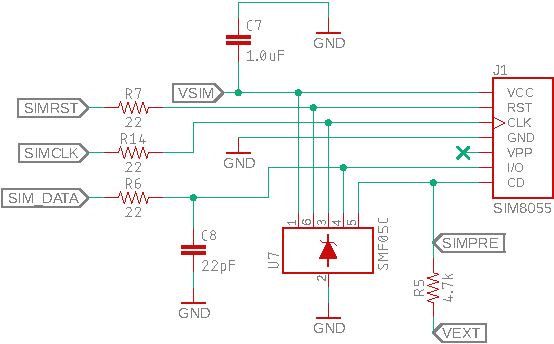
\includegraphics[width=\textwidth]{GSM_SIM_esquem.pdf}
\caption{Esquemático del módulo SIM8055.}
\label{fig:GSM_SIM_esquem}
\end{figure}

Por último, se tiene en la Fig.~\ref{fig:GSM_LED_esquem} el esquemático de la conexión de dos LEDs que servirán para indicar el estado de la conexión a Internet del módulo y también si este se encuentra encendido o no. Se usará un conector para cablear los LEDs ya que estos no se encontrarán soldados a la PCB porque se necesitan en una posición específica del case del dispositivo.

\begin{figure}[htbp!]
\centering
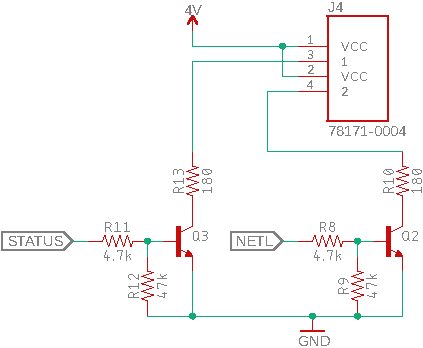
\includegraphics[width=0.7\textwidth]{GSM_LED_esquem.pdf}
\caption{Esquemático las los indicadores LED.}
\label{fig:GSM_LED_esquem}
\end{figure}



\subsubsection{Pantalla}
La pantalla se colocará fuera del case donde estará el PCB por lo que se usarán borneras para conectar los pines necesarios al microcontrolador, como indica la Fig.~\ref{fig:DISPLAY_esquem}. Se usa el protocolo SPI para comunicarse con el microcontrolador y se alimenta a la pantalla con \SI{3.3}{V}. Además se usan solo 8 pines ya que estos son los únicos necesarios para controlar la pantalla.

\begin{figure}[htbp!]
\centering
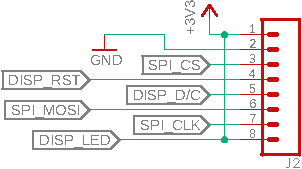
\includegraphics[width=0.6\textwidth]{DISPLAY_esquem.pdf}
\caption{Esquemático bornera para conectar la pantalla.}
\label{fig:DISPLAY_esquem}
\end{figure}


\subsubsection{Microcontrolador}
En la Fig.~\ref{fig:ESP_esquem} se muestra el esquemático del microcontrolador y su alimentación. En la hoja de datos \cite{Esp32_Hardware} se recomienda usar los capacitores que se encuentran conectados al microcontrolador y se muestran también todas las conexiones de los módulos anteriores; 1 conexión I\textsuperscript{2}C, 2 conexiones seriales y 1 conexión SPI.

\begin{figure}[hbtp!]
\centering
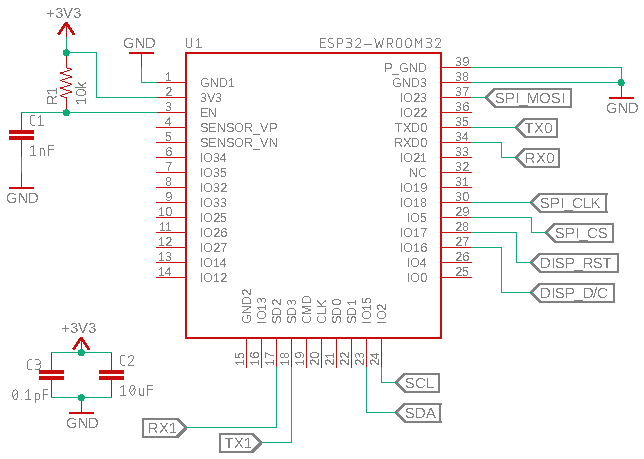
\includegraphics[width=\textwidth]{ESP32_esquem.pdf}
\caption{Esquemático de la implementación del ESP-WROOM-32.}
\label{fig:ESP_esquem}
\end{figure}


\subsubsection{Regulador swtiching}
En la Fig.~\ref{fig:esquem_switching} se puede observar la selección de los componentes externos al TPS563210 usados para obtener una salida de \SI{4}{V} de una fuente de \SI{12}{V}. El primer paso para seleccionar estos componentes fue determinar el voltaje de salida requerido (\SI{4}{V}). En \cite{TPS563210} se tiene que el V\textsubscript{out} seguirá la Ecuación~\ref{eq:vout}.
\begin{figure}[hbtp!]
\centering
\makebox[\textwidth][c]{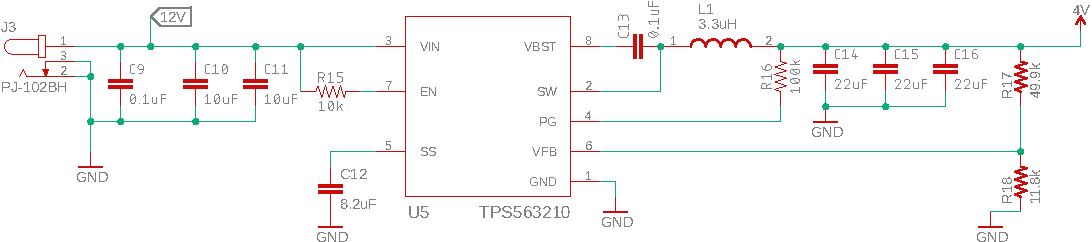
\includegraphics[width=\textwidth]{Switching.pdf}}%
\caption{Esquemático de la implementación del TPS563210.}
\label{fig:esquem_switching}
\end{figure}

\begin{equation}
    V_{out}=0.765\times(1+\frac{R_{17}}{R_{18}})
    \label{eq:vout}
\end{equation}

Para asegurar que $V_{out}=\SI{4}{V}$ se usan resistencias de la serie E96 (con 1\% de tolerancia en su valor). Los valores de $R_{17}$ y $R_{18}$ que cumplen con esta ecuación son $R_{17}=\SI{49.9}{k\ohm}$ y $R_{17}=\SI{11.8}{k\ohm}$.

Luego se recomienda en \cite{TPS563210} usar una inductancia de valor $L_1=\SI{3.3}{\micro H}$ y el IC usa una frecuencia de $f_{SW}=\SI{650}{kHz}$. Además se necesita el valor máximo que el voltaje de entrada V\textsubscript{in} puede tomar, que en este caso será $V_{in}=\SI{16}{V}$ (Esto es debido a fluctuaciones en el voltaje de la batería). Con estos valores se puede determinar los parámetros $Il_{P-P}$, $Il_{PEAK}$,  $I_{LO(RMS)}$ y $I_{CO}$ con las ecuaciones:
\begin{align}
Il_{P-P}&=\frac{V_{out}}{V_{in(MAX)}}\times\frac{V_{in(MAX)}-V_{OUT}}{L_O\times f_{SW}} \label{eq:current1}\\
Il_{PEAK}&=I_{o}+\frac{Il_{P-P}}{2} \label{eq:current2}\\
I_{LO(RMS)}&=\sqrt{I_o^2+\frac{1}{12}Il_{P-P}^2} \label{eq:current3} \\
I_{CO}&=\frac{V_{out}\times (V_{in}-V_{out})}{\sqrt{12}\times V_{in}\times L_{O} \times f_{Sw}} \label{eq:current4}
\end{align}

El resultado de las Ecuaciones \ref{eq:current1}, \ref{eq:current2}, \ref{eq:current3} y \ref{eq:current4} son:
\begin{align*}
Il_{P-P}&=\SI{1.398}{A} &
Il_{PEAK}&=\SI{3.319}{A}&
I_{LO(RMS)}&=\SI{2.79}{A} &
I_{CO(RMS)}&=\SI{0.02}{A}
\end{align*}

Se selecciona entonces el inductor CLF7045NIT-3R3N-D de \SI{3.3}{\micro H} que soporta los parámetros mencionados anteriormente \cite{Inductor} y 3 capacitores C3216X5R0J226M en la salida de \SI{22}{\micro F}  que soporta hasta \SI{4}{A} RMS. Los capacitores de entrada y las demás resistencias se colocan por recomendación de \cite{TPS563210}.


\subsubsection{Regulador LDO}

En la Fig.~\ref{fig:LDO} se puede observar la selección de componentes externos y el esquemático propuesto para el LT1764A. Los capacitores C\textsubscript{17} y C\textsubscript{18} toman valores recomendados en la hoja de datos \cite{LT1764A}

\begin{figure}[hbtp!]
\centering
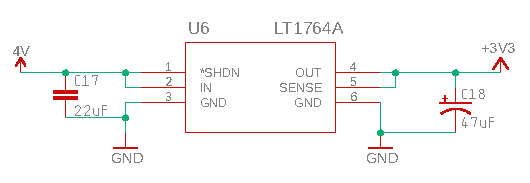
\includegraphics[width=\textwidth]{LDO.pdf}
\caption{Esquemático de la implementación del LT1764A.}
\label{fig:LDO}
\end{figure}









\subsection{Diseño del PCB}
A continuación se incluirá el diseño del PCB en el que irán todos los componentes antes mencionados. Como se aprecia en la Fig.~\ref{fig:Board}, el PCB cuenta con dos capas. La capa inferior cuenta con un plano de GND que ayudará no solo a conectar los componentes más fácilmente sino que es recomendado por algunos de los componentes como el SIM 800L \cite{SIM800L}.

\begin{figure}[hbtp!]
\centering
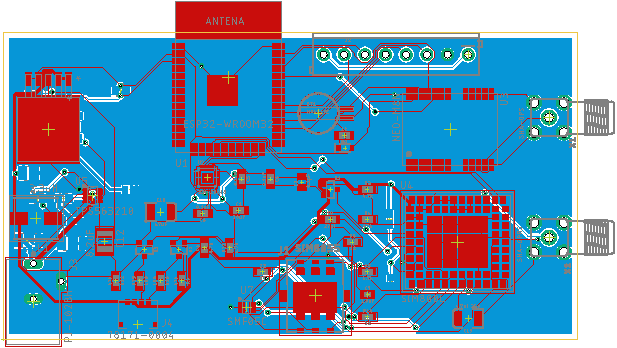
\includegraphics[width=\textwidth]{Board.pdf}
\caption{Diseño del PCB.}
\label{fig:Board}
\end{figure}


En la Fig.~\ref{fig:board_top} se puede apreciar la parte superior del PCB con sus dimensiones en mm y en la Fig.~\ref{fig:board_bottom} se aprecia la parte inferior

\begin{figure}[hbtp!]
\centering
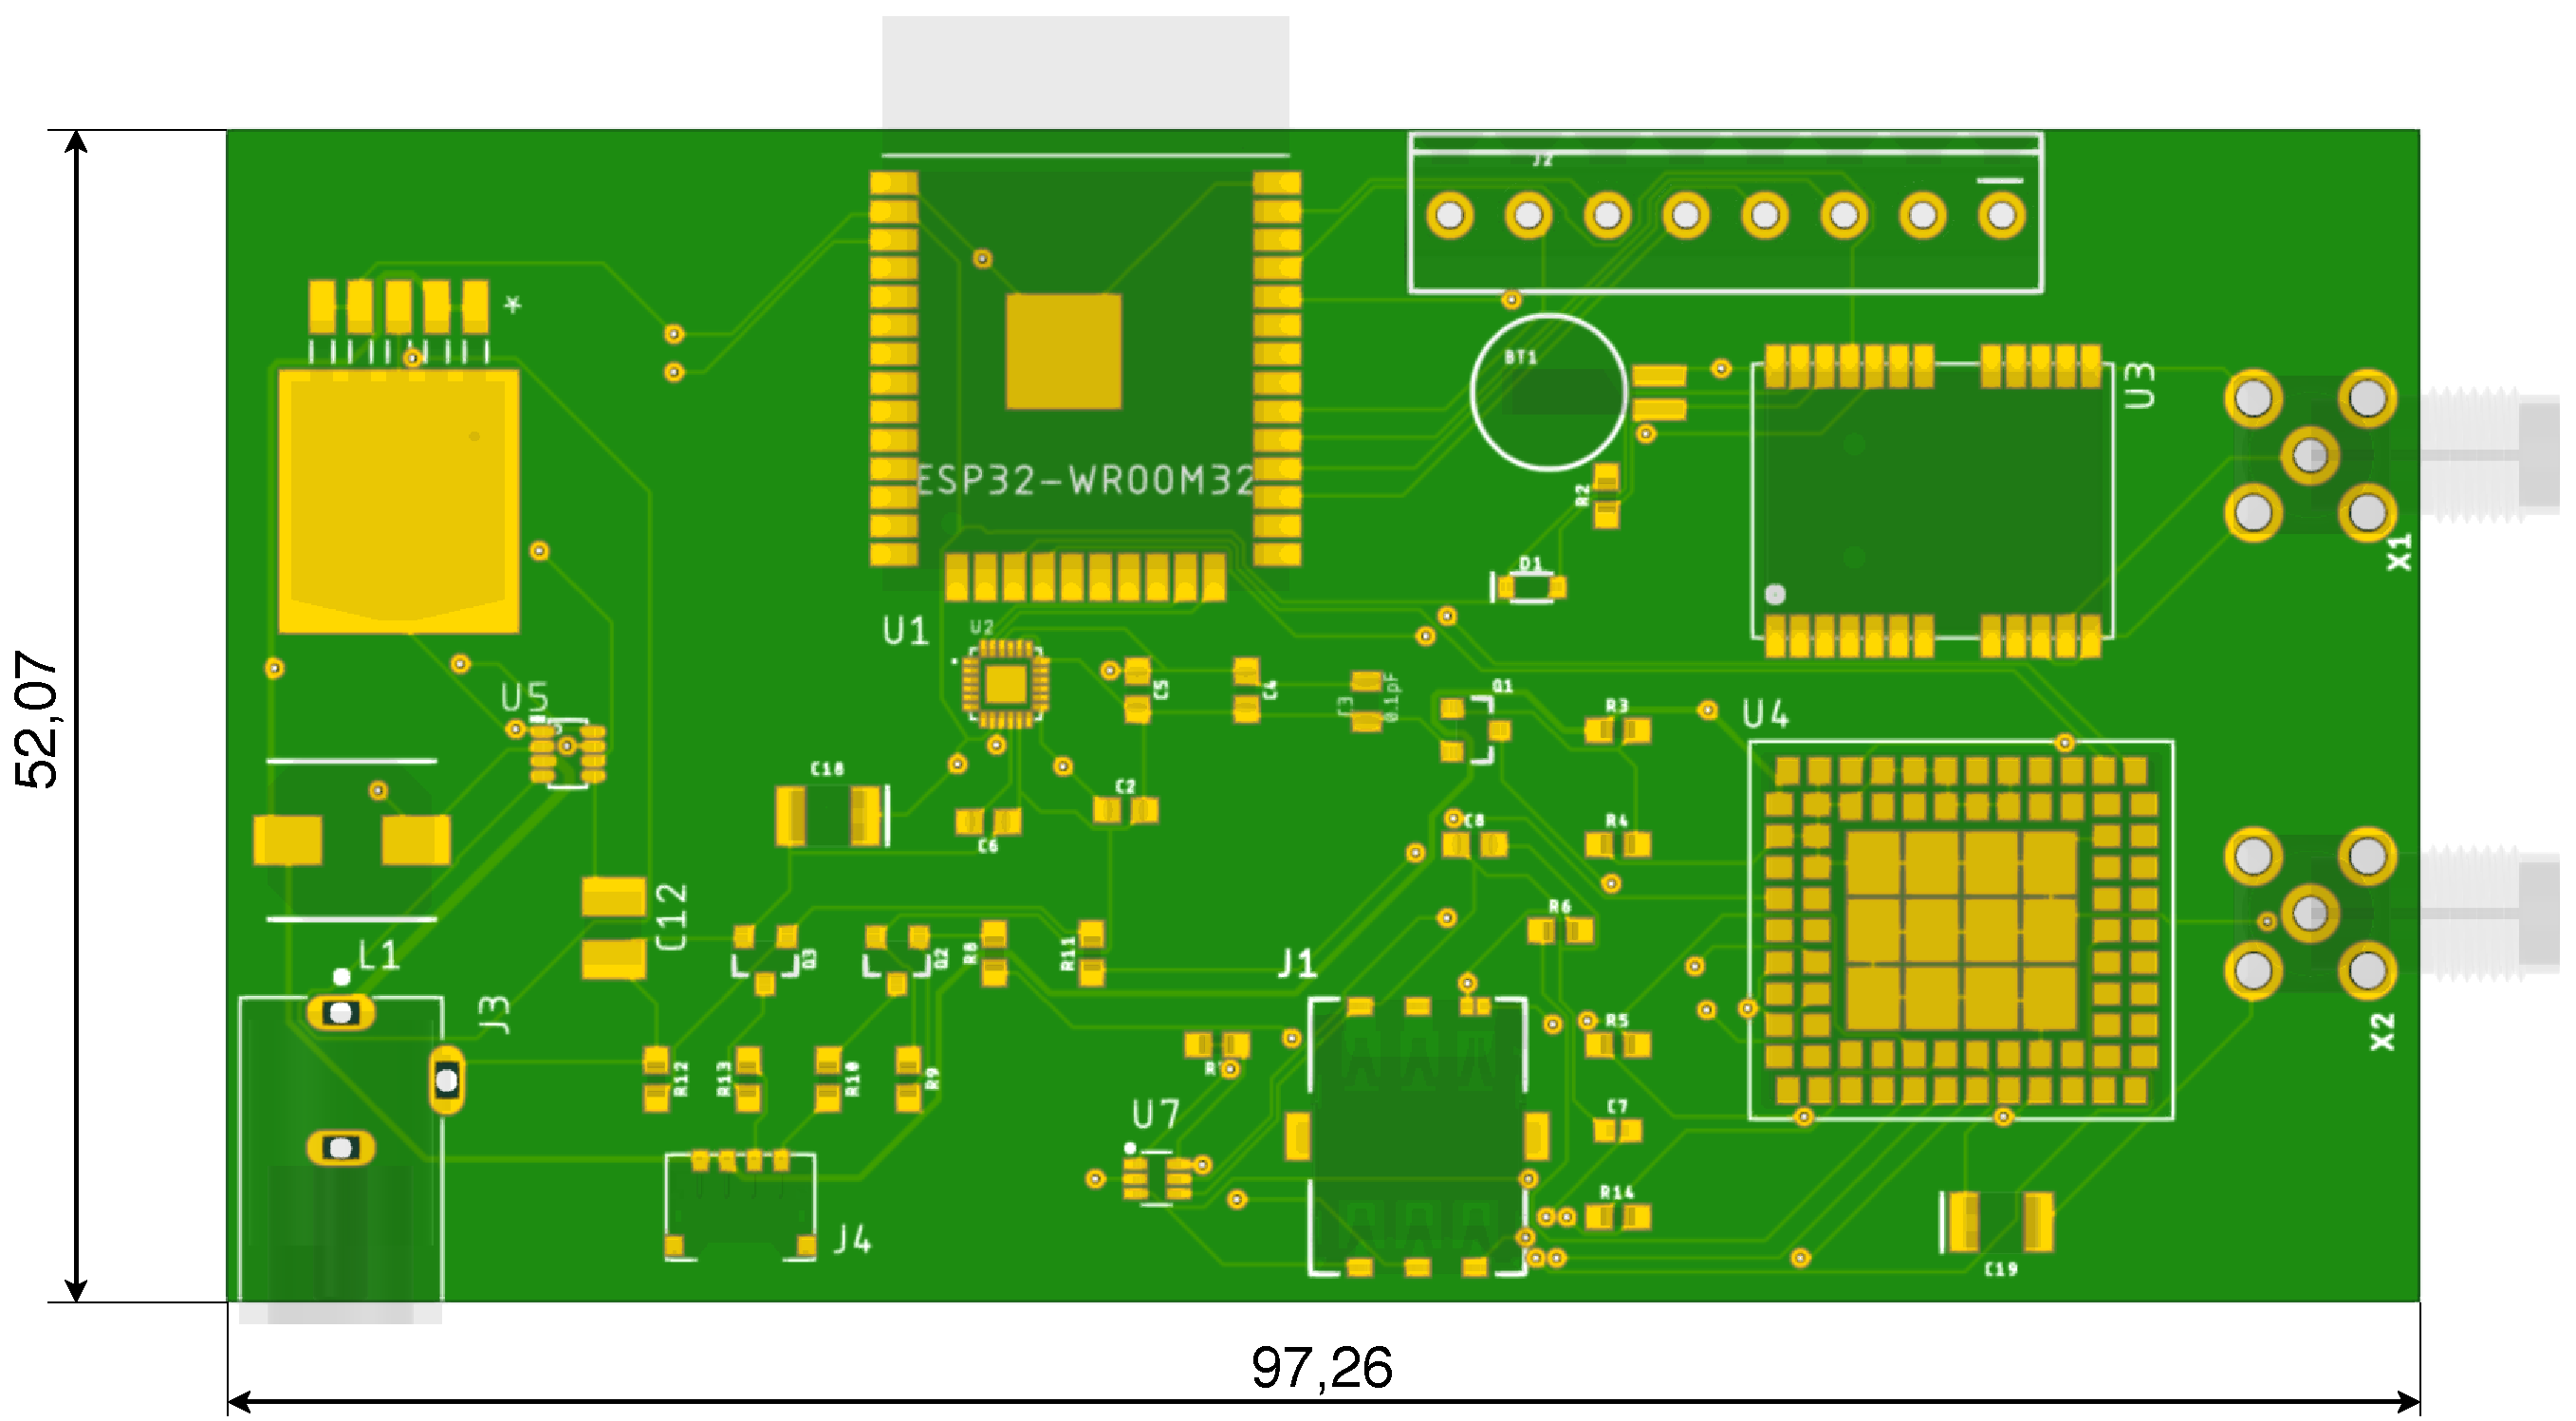
\includegraphics[width=\textwidth]{board_top_dim.pdf}
\caption{Parte superior del PCB.}
\label{fig:board_top}
\end{figure}

\begin{figure}[hbtp!]
\centering
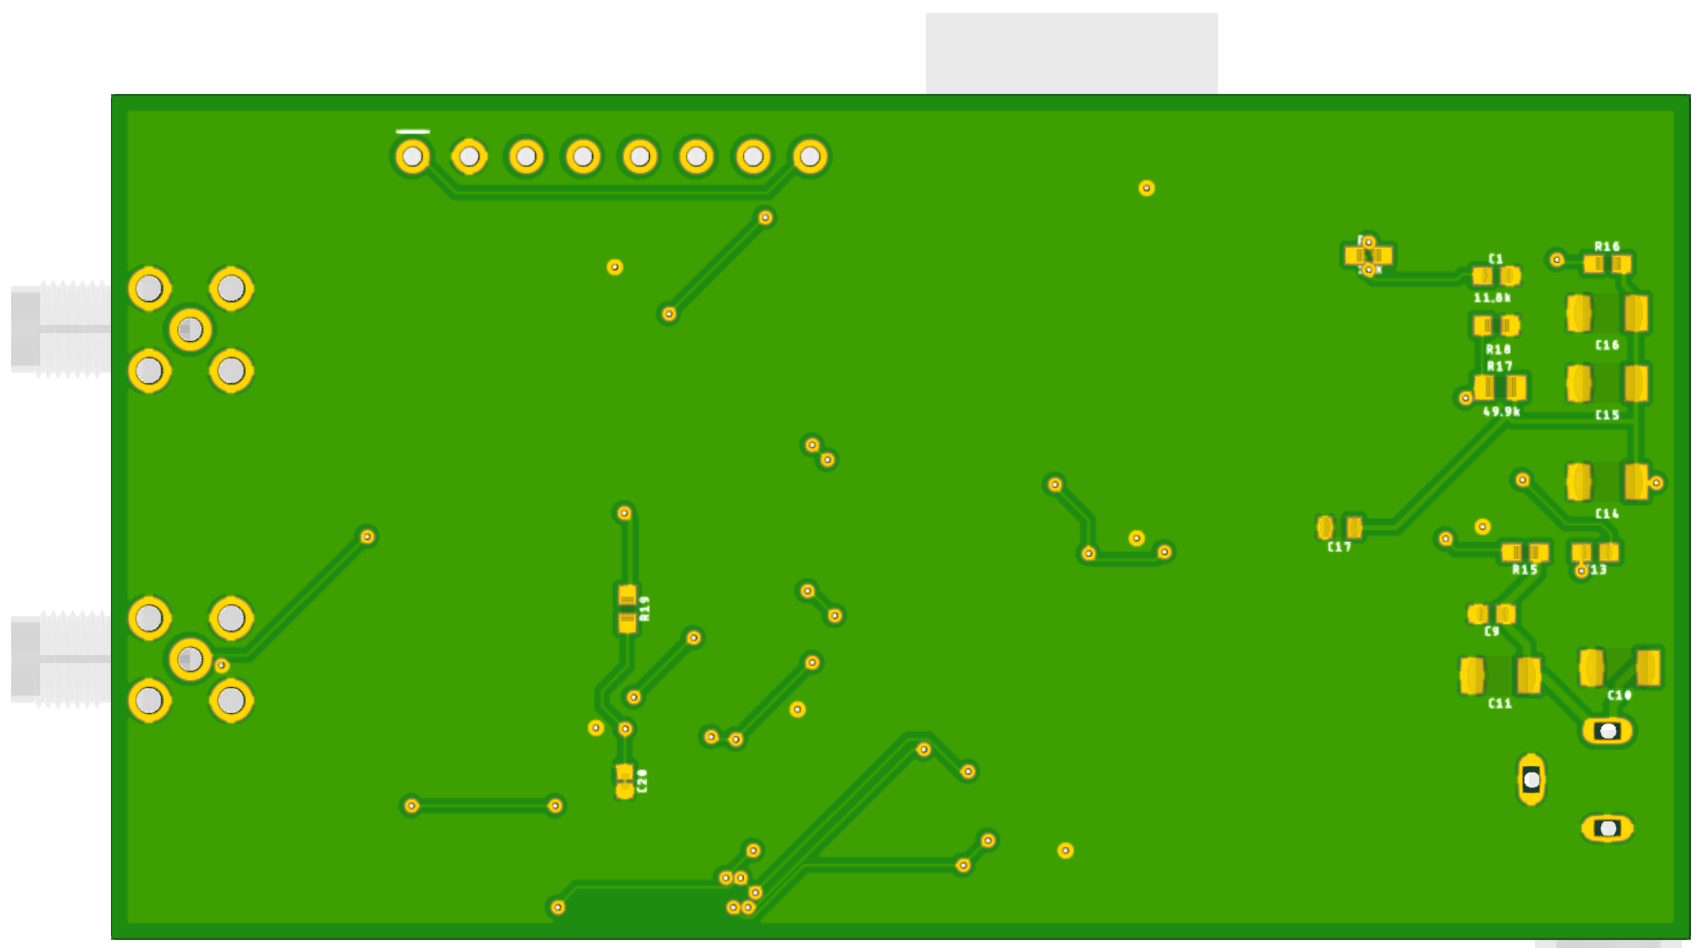
\includegraphics[width=\textwidth]{board_bottom.png}
\caption{Parte inferior del PCB.}
\label{fig:board_bottom}
\end{figure}

Se tuvo una consideración importante al escoger el ancho de las pistas que se encuentran en este PCB. Siguiendo la Fig.~\ref{fig:bloques_alim}, en donde se pueden ver las corrientes máximas que se alcanzarán. Se tienen pistas por donde pasarán \SI{2.6}{A}, \SI{2}{A} y \SI{0.62}{A}. Para poder elegir el ancho adecuadamente se utiliza la Ecuación~\ref{eq:width1} en dónde $I$ es la máxima corriente permisible, $\Delta T$ es el incremento de temperatura permisible y $A$ es la sección transversal de la pista.

\begin{equation}
    I = k\Delta T^{0.44}A^{0.725}
    \label{eq:width1}
\end{equation}

Si expresamos $A=Espesor\times Ancho$ Y despejamos $Ancho$, obtendríamos la Ecuación~\ref{eq:width2}

\begin{equation}
    Ancho = \left(\frac{I}{k\Delta T^{0.44}}\right)^{\frac{1}{0.725}}\times \frac{1}{Espesor}
    \label{eq:width2}
\end{equation}


Al usar la Ecuación~\ref{eq:width2} con $\Delta T=\SI{20}{\celsius}$, y un espesor de pista de \SI{1}{oz/ft^2} se tienen los mínimos anchos de pista necesarios para cada corriente mencionada. Los resultados se observan en la Tabla~\ref{diag:traces_width}. Sin embargo, estos son solo los anchos mínimos. Es por eso que para una corriente de \SI{620}{mA} o menor se usará un ancho de pista de \SI{10}{mil} por defecto y de \SI{6}{mil} para soldar los pads del SIM 800L.

\bgroup
\def\arraystretch{1.5}%  1 is the default, change whatever you need
\begin{table}[htbp!]
\centering
\caption[Anchos de pista mínimos]{Anchos de pista mínimos.}
\begin{tabular}{@{}ll@{}}
\toprule
Corriente máxima & Ancho mínimo \\ \midrule
\SI{2.6}{A} & \SI{29}{mil} \\
\SI{2}{A} & \SI{20.2}{mil} \\
\SI{620}{mA} & \SI{4}{mil} \\ \bottomrule
\end{tabular}
\label{diag:traces_width}
\end{table}
\egroup

El PCB diseñado tiene componentes que exceden las dimensiones de la placa. Las dimensiones con componentes se puede apreciar en las Figuras \ref{fig:board_top_con},  \ref{fig:board_bottom_con} y \ref{fig:board_side_con}

\begin{figure}[hbtp!]
\centering
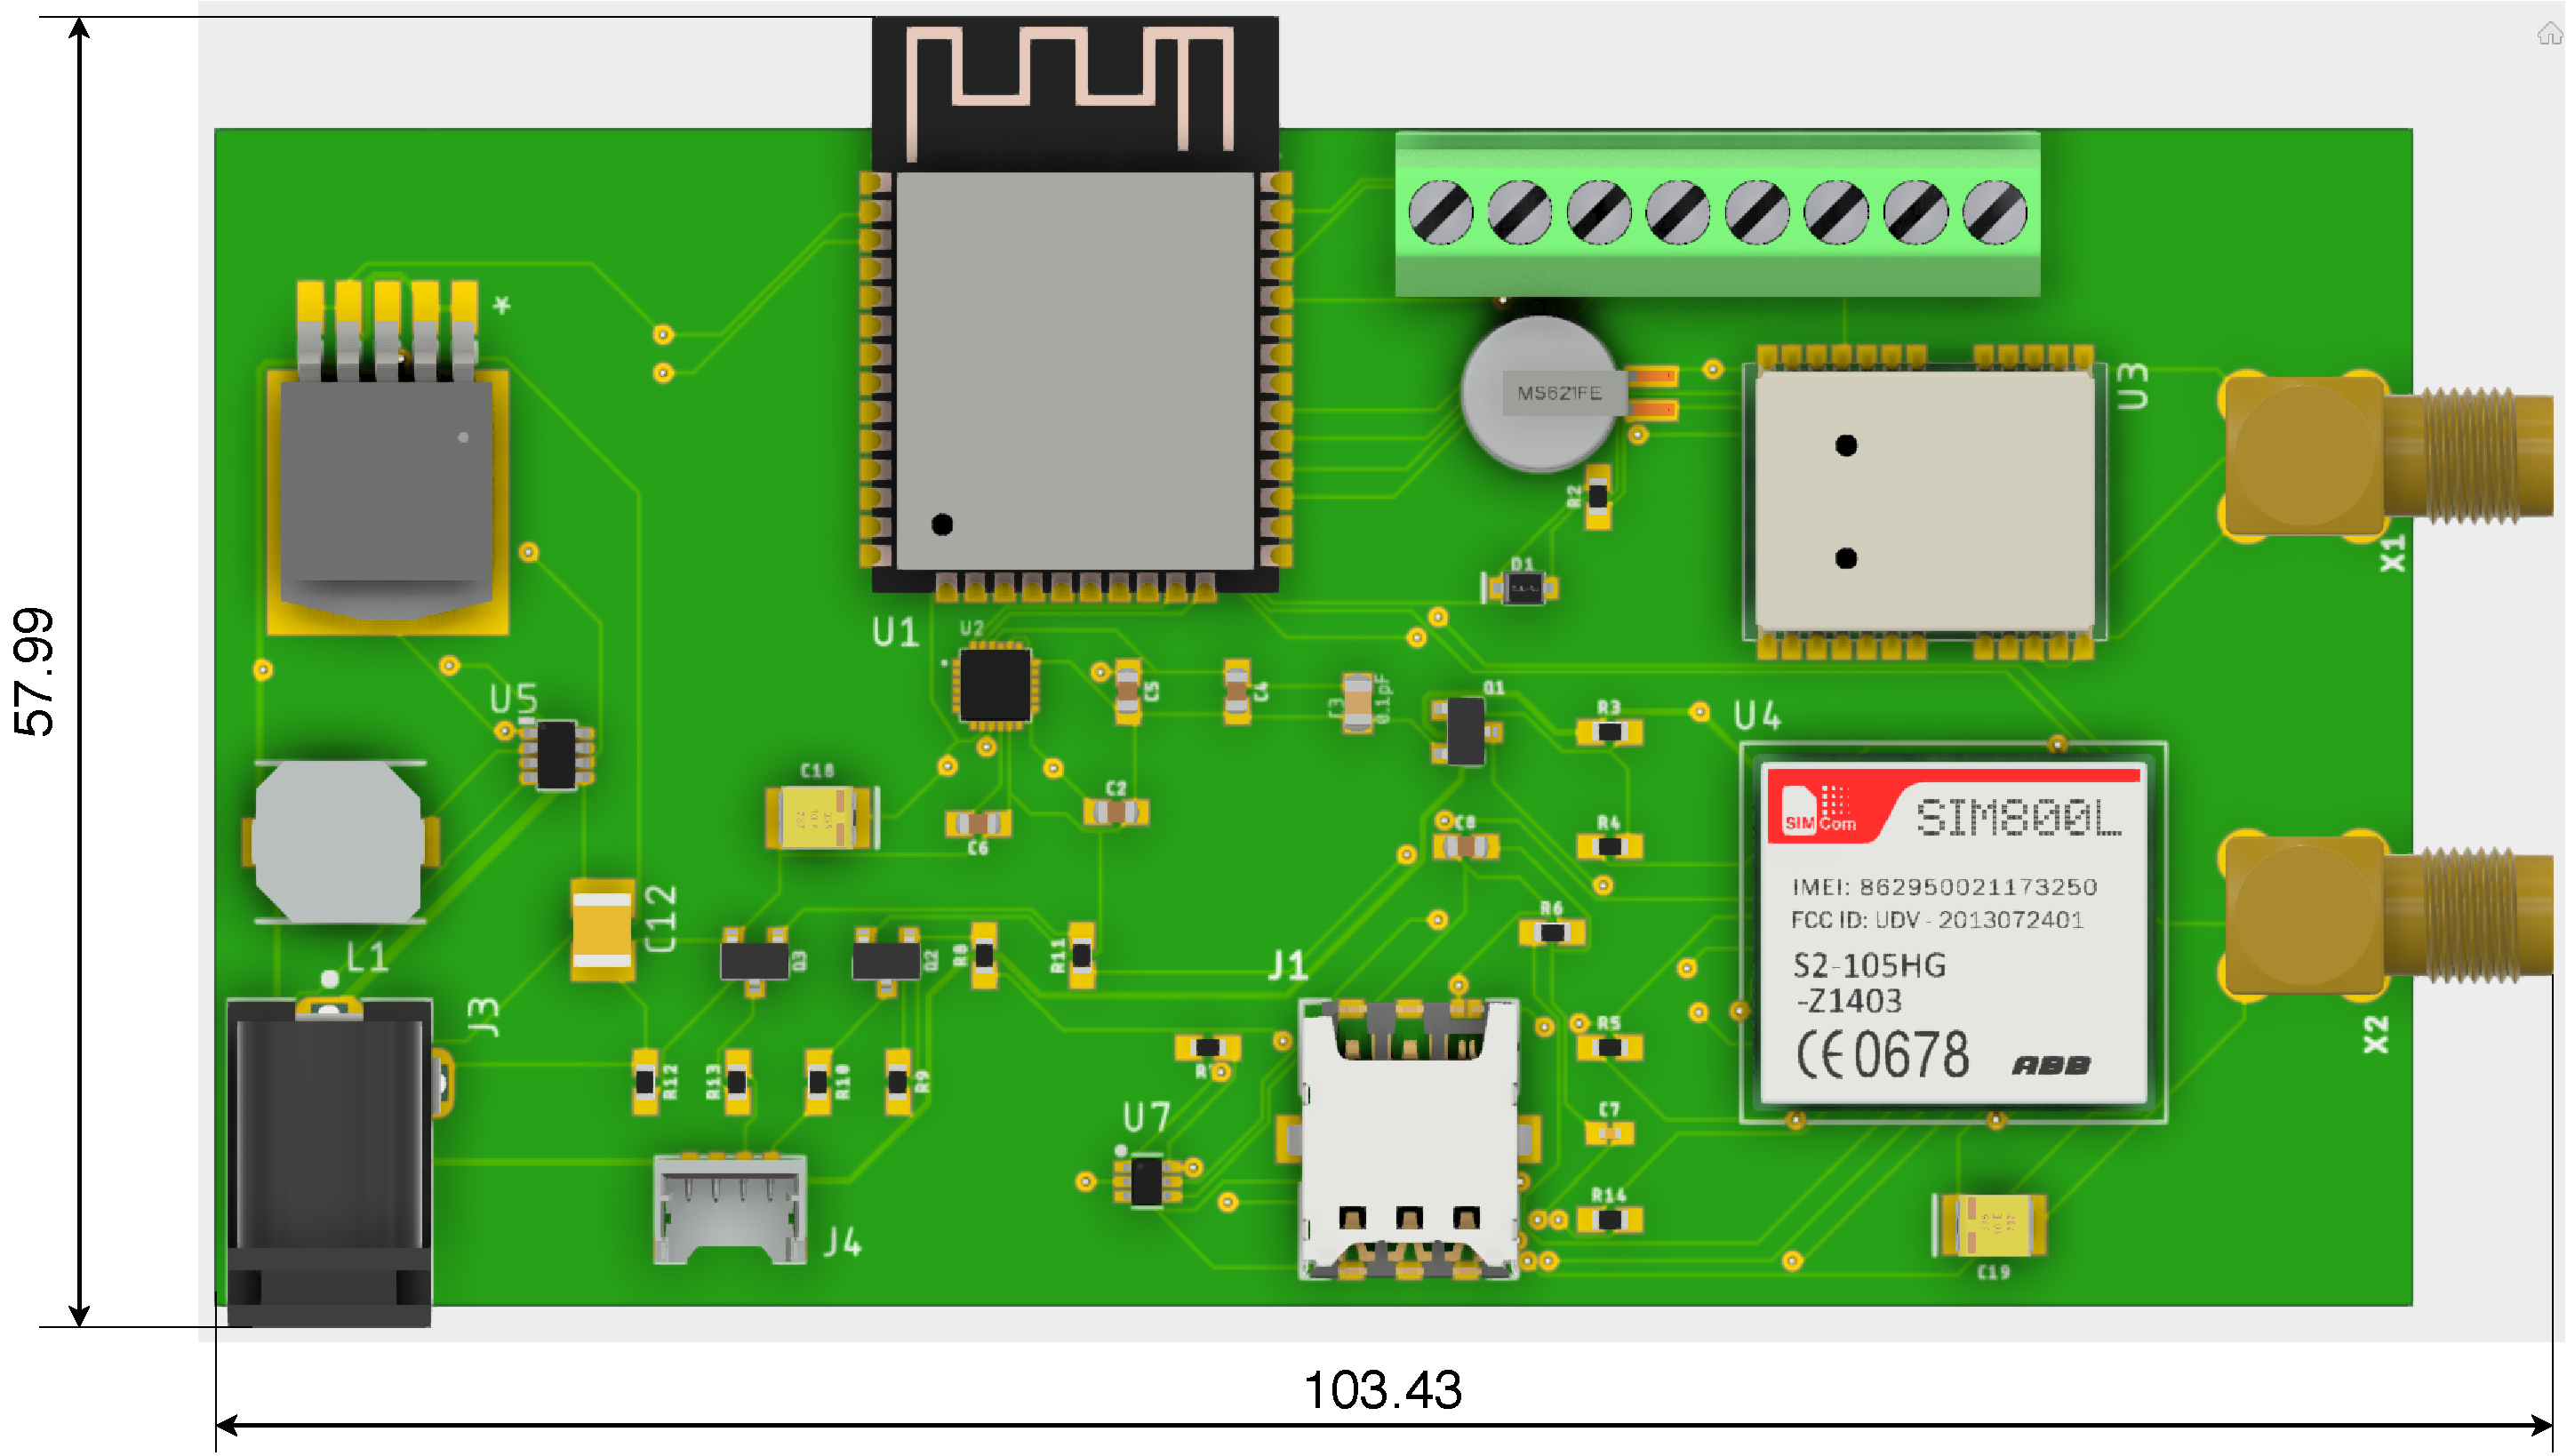
\includegraphics[width=\textwidth]{board_top_com_dim.pdf}
\caption{Parte superior del PCB con componentes.}
\label{fig:board_top_con}
\end{figure}

\begin{figure}[hbtp!]
\centering
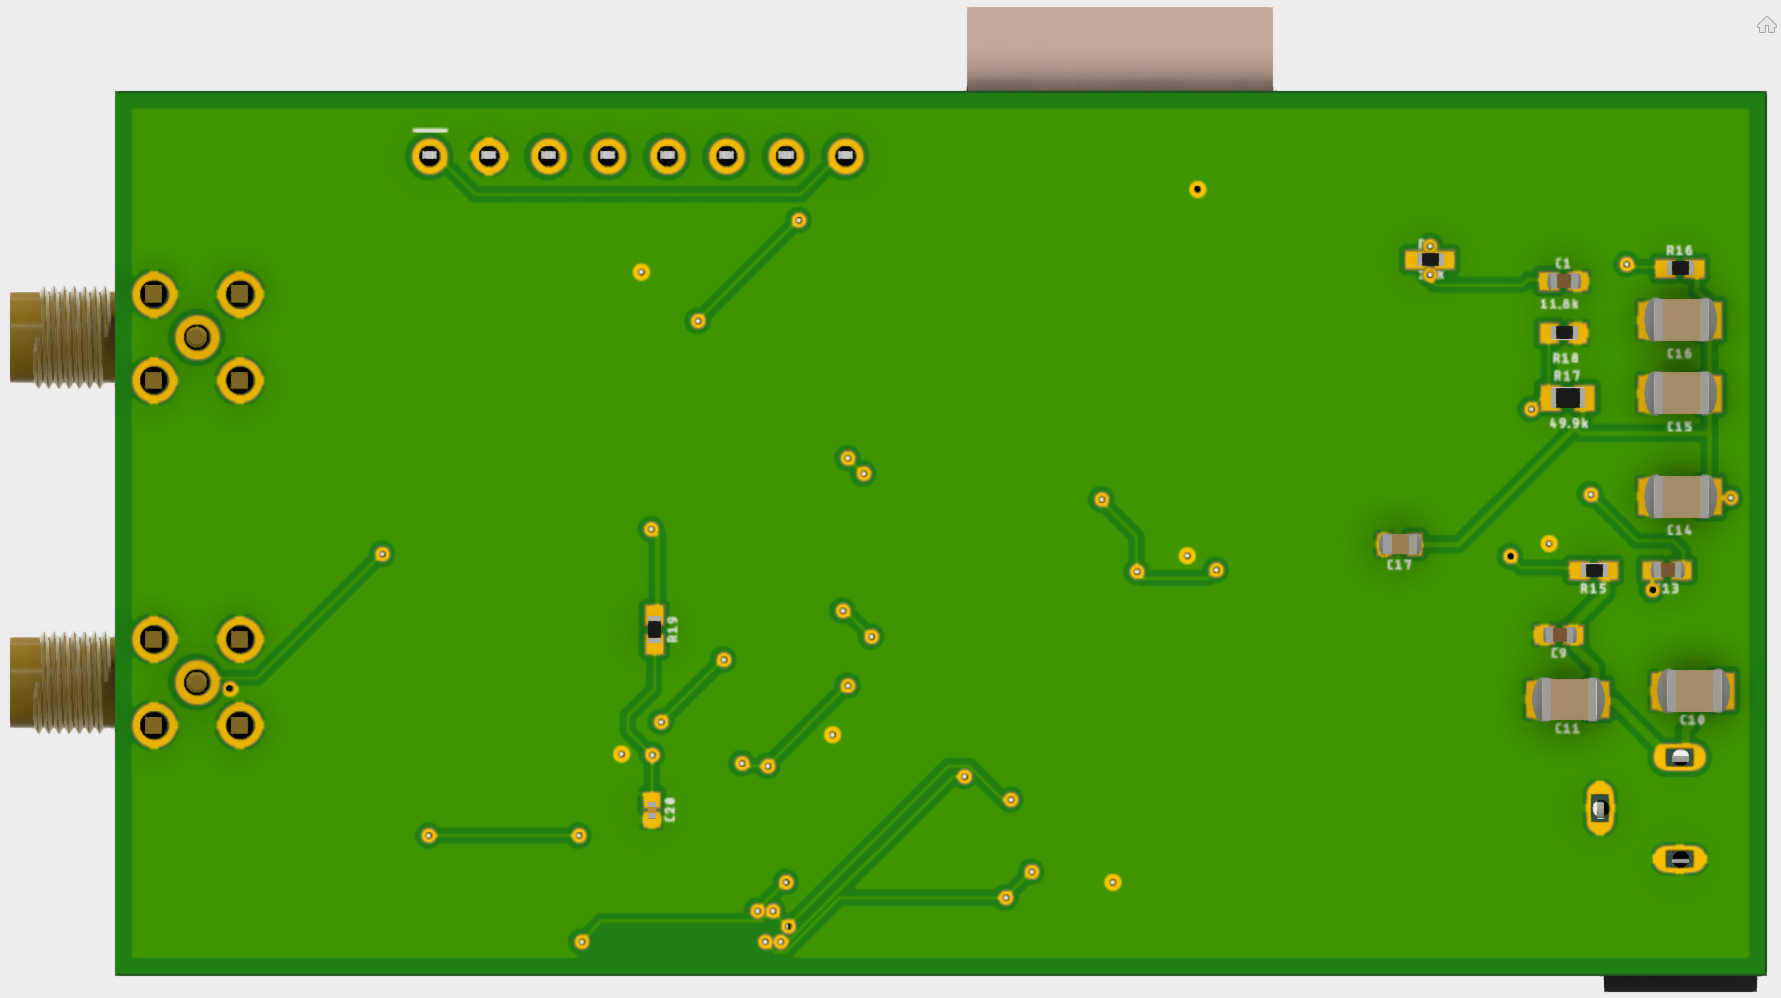
\includegraphics[width=\textwidth]{board_com_bottom.png}
\caption{Parte inferior del PCB con componentes.}
\label{fig:board_bottom_con}
\end{figure}

\begin{figure}[hbtp!]
\centering
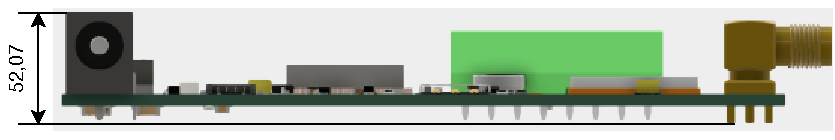
\includegraphics[width=\textwidth]{board_side_dim.pdf}
\caption{Vista lateral del PCB.}
\label{fig:board_side_con}
\end{figure}


\section{Diseño mecánico}
En este capítulo se describirán los planos de ensamble y despiece y se seleccionarán los componentes mecánicos y materiales a usar.

\subsection{Diseño del Case Principal}

El PCB antes diseñado será colocado en un case que se fabricará usando impresión 3D de dimensiones $\SI{63}{mm} \times \SI{108}{mm} \times \SI{28}{mm}$. El case contará con una entrada de alimentación de 2.5 mm, una ranura para una tarjeta nano SIM, dos conectores SMA para conectar las antenas de GPS y GPRS/GSM y por último 2 indicadores LED que indicarán el encendido del dispositivo y su conexión a Internet. Todos estos elementos se pueden observar en las Fig.~\ref{fig:exploded}.

\begin{figure}[hbt!]
\centering
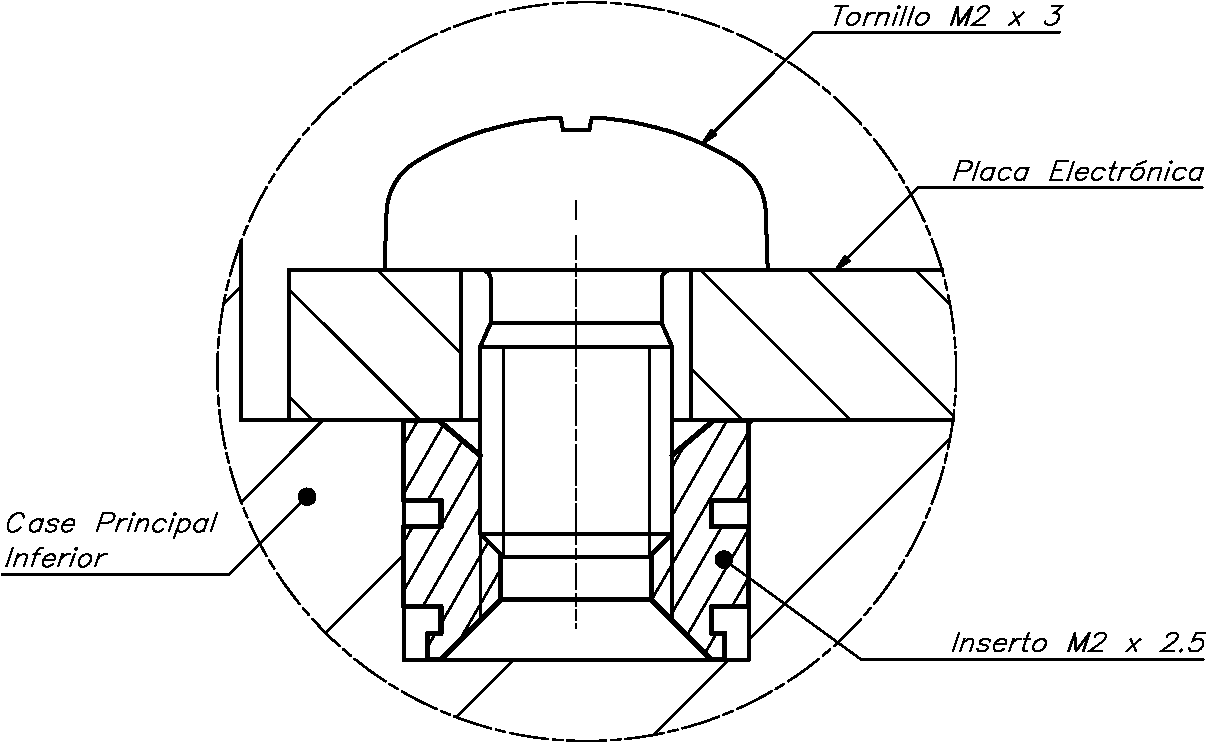
\includegraphics[width=0.8\textwidth]{union_atornillada.pdf}
\caption{Unión de la tarjeta electrónica con el case.}
\label{fig:ensamble_principal}
\end{figure}


\newpage

Este case cuenta con dos partes, una superior y otra inferior. En la inferior se ensamblará la tarjeta electrónica vista en el capítulo anterior. Esta unión (Fig.~\ref{fig:ensamble_principal}) se realizará usando una unión atornillada de un Tornillo M2 x 3 y un Inserto M2 x 2.5 que se coloca en un agujero en el case principal inferior.Este  inserto se puede observar en la Fig.~\ref{fig:insert} y esta diseñado para ser usado en plásticos (como el ABS).

\vspace{5mm}

\begin{figure} [hbt!]
\centering
\begin{minipage}{.5\textwidth}
  \centering
  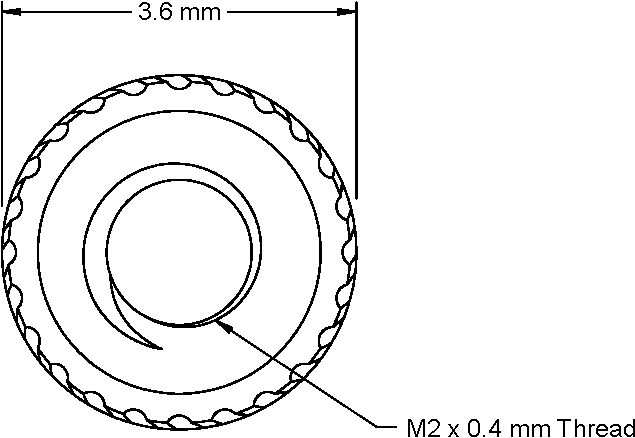
\includegraphics[width=.9\linewidth]{insert_1.pdf}
\end{minipage}%
\begin{minipage}{.5\textwidth}
  \centering
  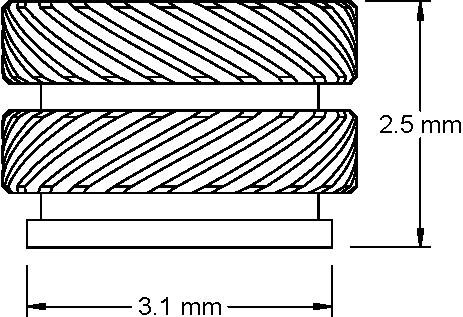
\includegraphics[width=.7\linewidth]{insert_2.pdf}
\end{minipage}
\caption{Inserto M2 x 2.5 para plástico.}
\label{fig:insert}
\end{figure}

Luego que la placa electrónica esta correctamente sujeta, se ensambla la parte superior del case. Para este ensamble se utilizan unas pestañas que encajarán entre si para facilitar el posicionamiento de las piezas y "snap fits" para la sujeción de las dos piezas. Esto se puede observar en la Fig.~\ref{fig:union-case_principal}.

Para el diseño de estás conexiones se tuvo en cuenta una separación de \SI{0.2}{mm} en las pestañas para asegurar que encajarán una con otra y que existirá un poco de fricción luego de ser impresas. Además se considero también una separación de \SI{0.3}{mm} en los snap fits para asegurar su posicionamiento.

\vspace{5mm}

\begin{figure}[hbt!]
\centering
\begin{subfigure}{.5\textwidth}
  \centering
  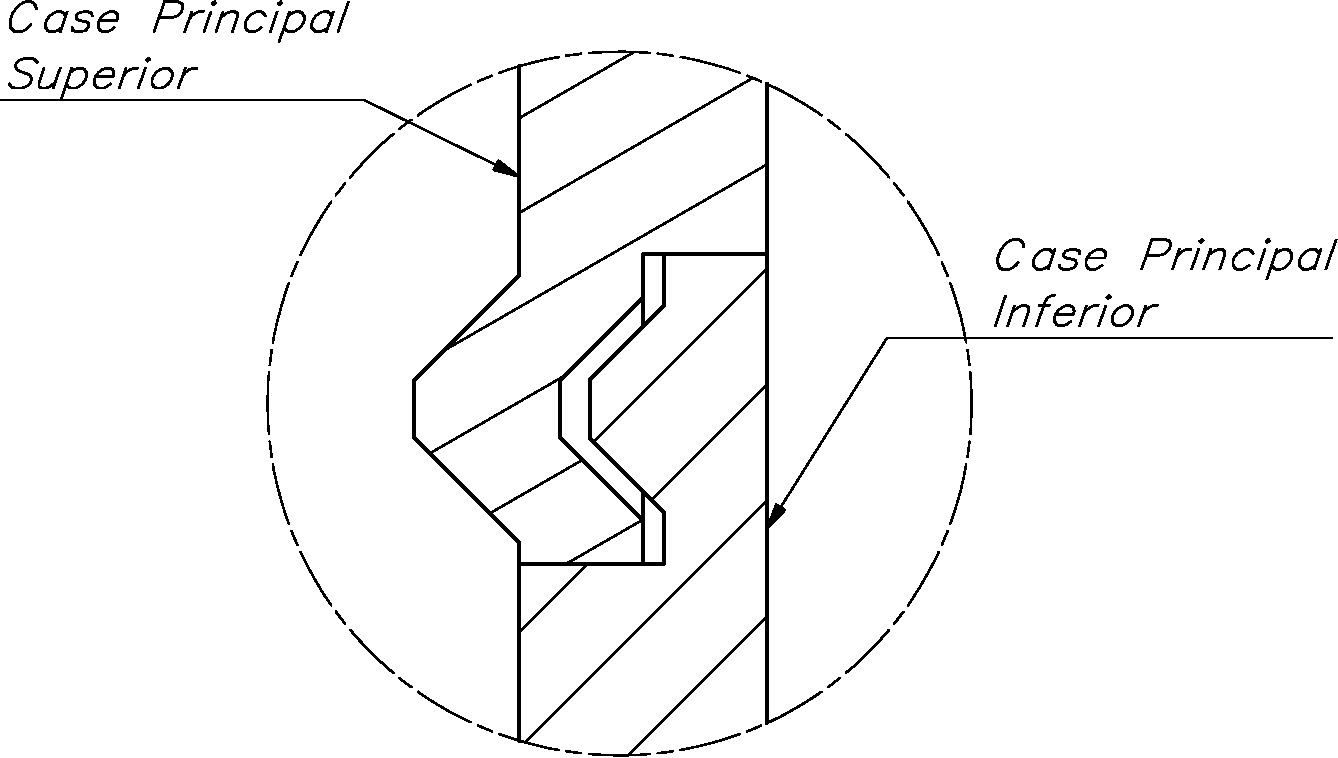
\includegraphics[width=\linewidth]{snap.pdf}
  \caption{Snap fits para la conexión}
  \label{fig:snaps_1}
\end{subfigure}%
\begin{subfigure}{.5\textwidth}
  \centering
  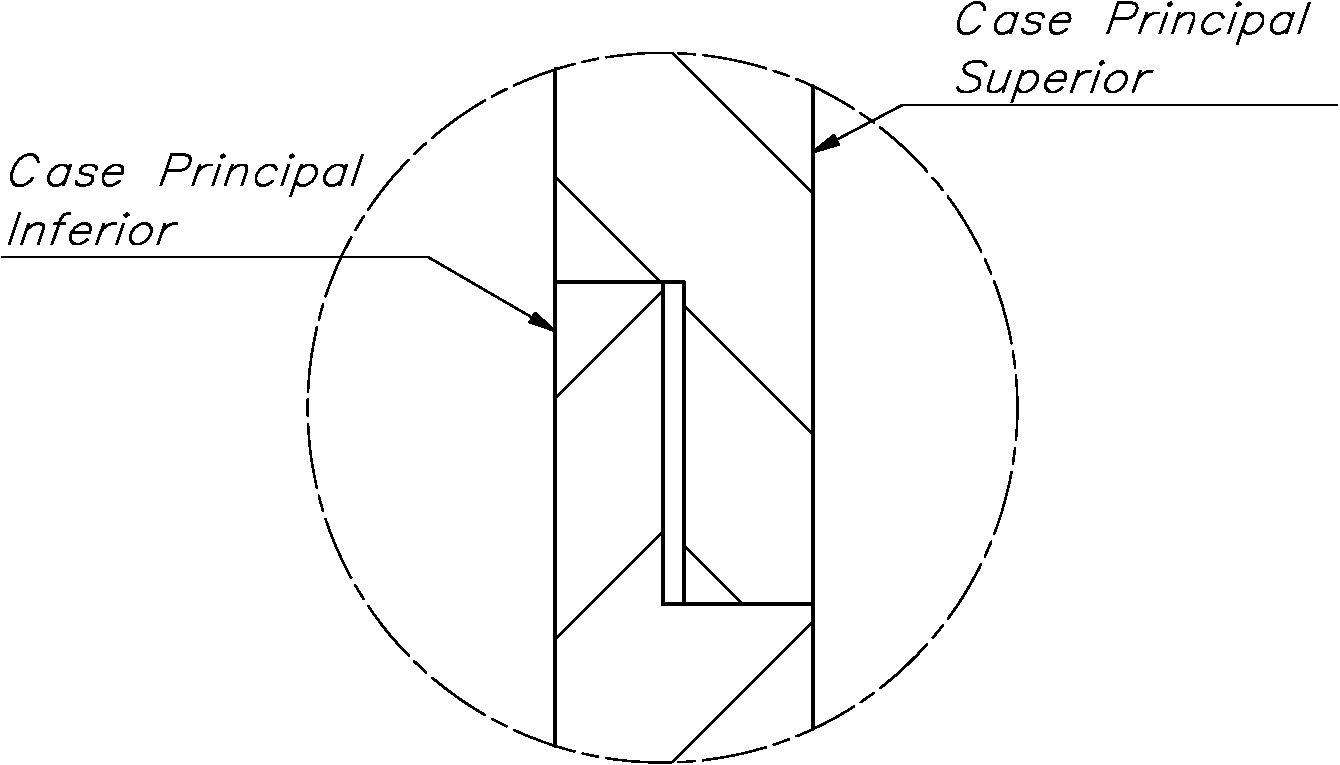
\includegraphics[width=0.9\linewidth]{lid.pdf}
  \caption{Pestañas para el posicionamiento}
  \label{fig:lid_1}
\end{subfigure}
\caption{Unión entre la parte superior e inferior del Case Principal}
\label{fig:union-case_principal}
\end{figure}

\newpage
\begin{figure}[hbt!]
\centering
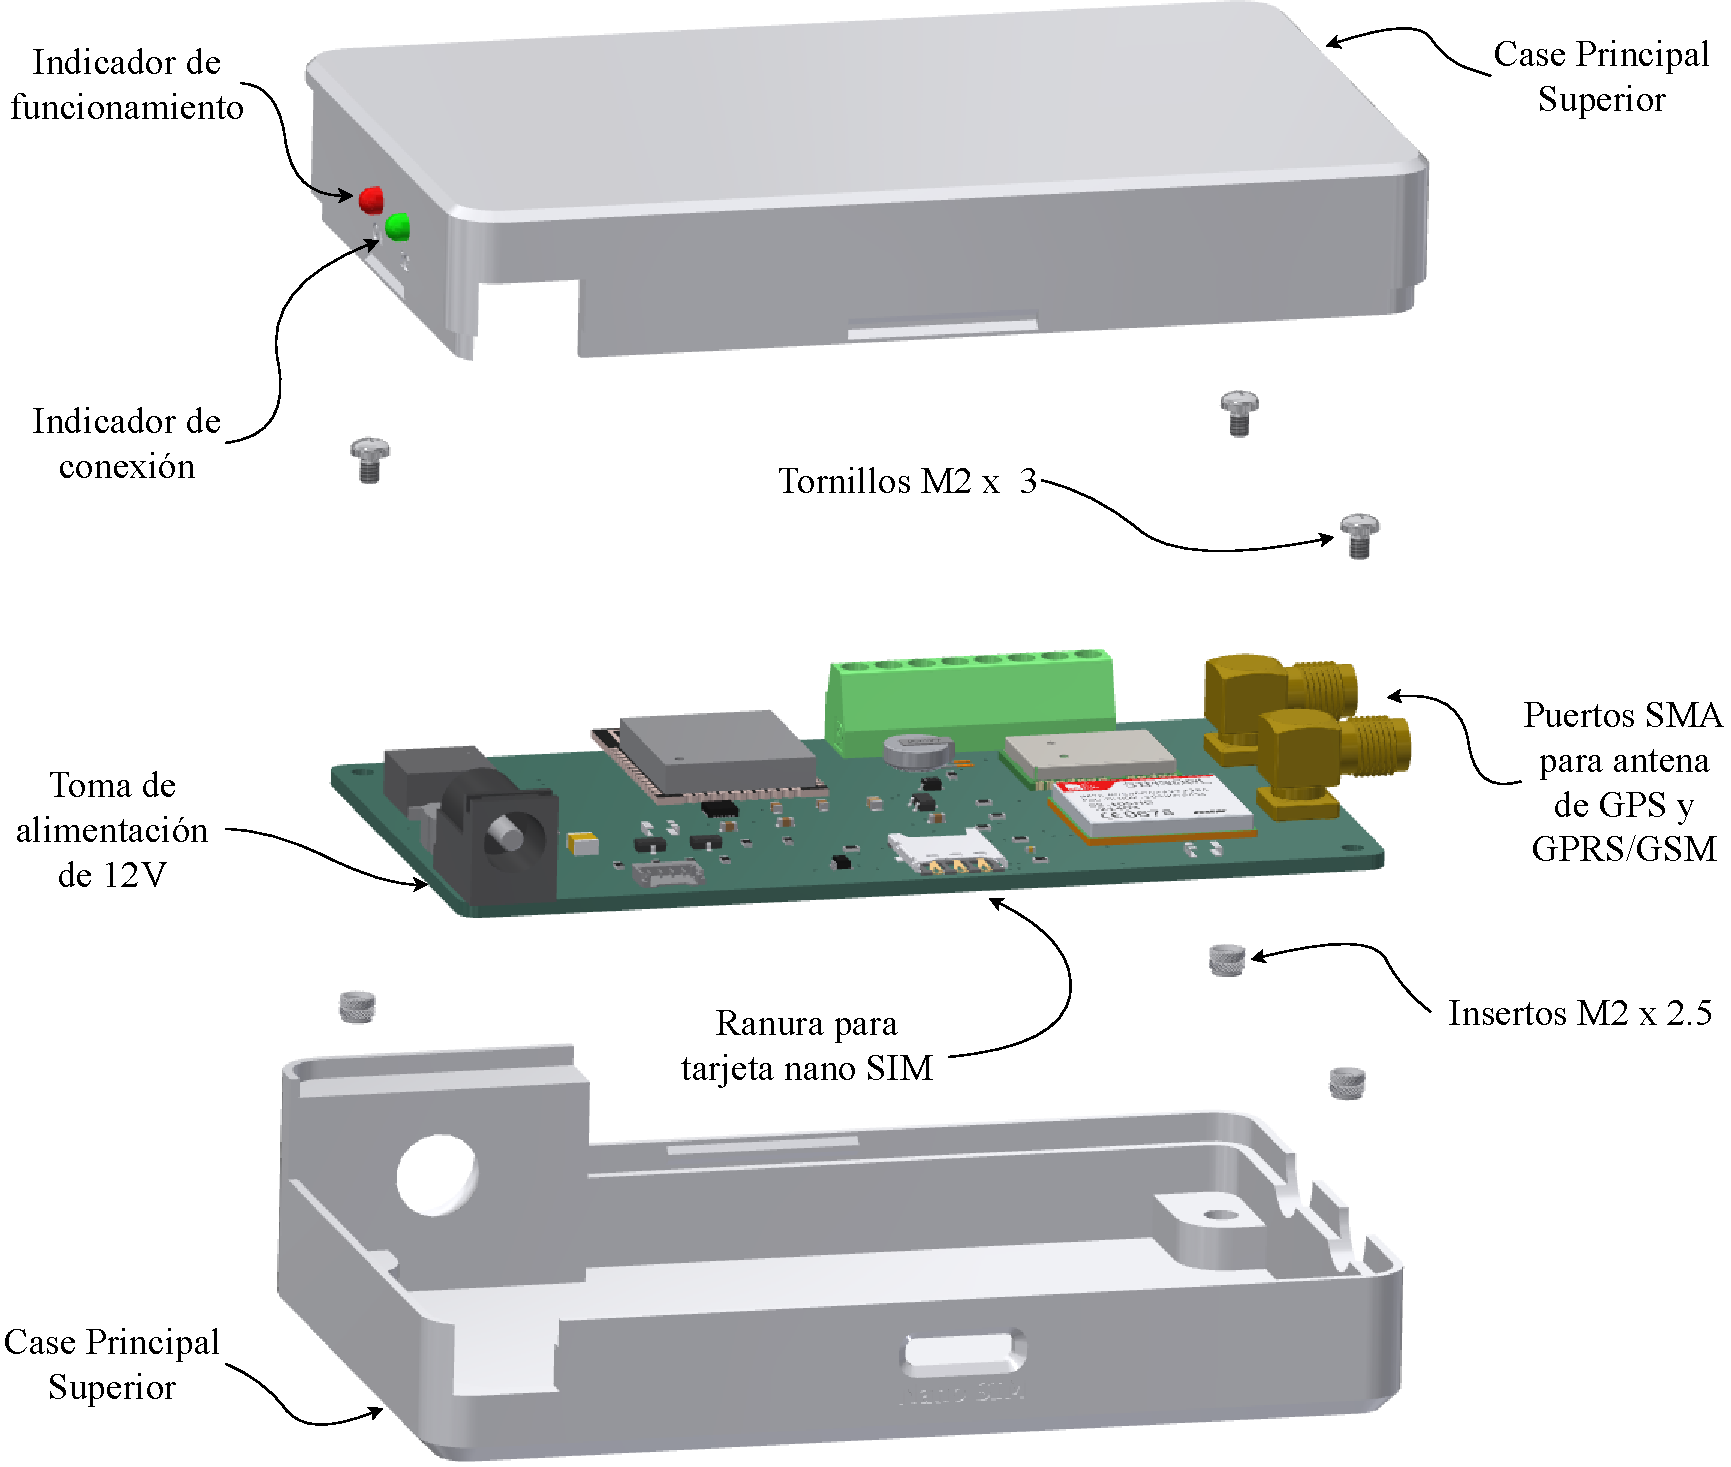
\includegraphics[width=\textwidth]{exploded.pdf}
\caption{Vista de explosión del case principal.}
\label{fig:exploded}
\end{figure}



%El case se diseñó teniendo en cuenta las limitaciones al usar ABS

%olerancias de impresión 3D de \SI{0.5}{mm} para que las piezas encajen sin problemas. El case se divide en dos partes. Estas partes encajan por forma y se atornillarán

%Para el ensamblaje de las dos partes del case se usan tornillos de rosca M2. Para la union atornillada se usan \textit{Inserts} metálicos para plástico que habilitan una rosca métrica.
%\subsection{Diseño del Case de la pantalla}
\subsection{Selección del brazo de la pantalla}

Para seleccionar el brazo que sujete la pantalla se tienen en cuenta dos requerimientos:
\vspace{-3mm}
\begin{itemize}
    \itemsep0pt
    \item La posición de la pantalla debe ser regulable por el conductor.
    \item Los cables tienen que poder ser conducidos a través del brazo hacia la pantalla
\end{itemize}

Se usarán entonces las mangueras a piezas de la marca \textit{Loc-Line} (Fig.~\ref{fig:brazo_1}). Estas mangueras se componen de múltiples piezas huecas, cada una se une a la siguiente por medio de una articulación de rótula. PONER AQUI UNA IMAGEN Y DESCRIPCION DE LA ROTULA

\begin{figure}[hbt!]
\centering
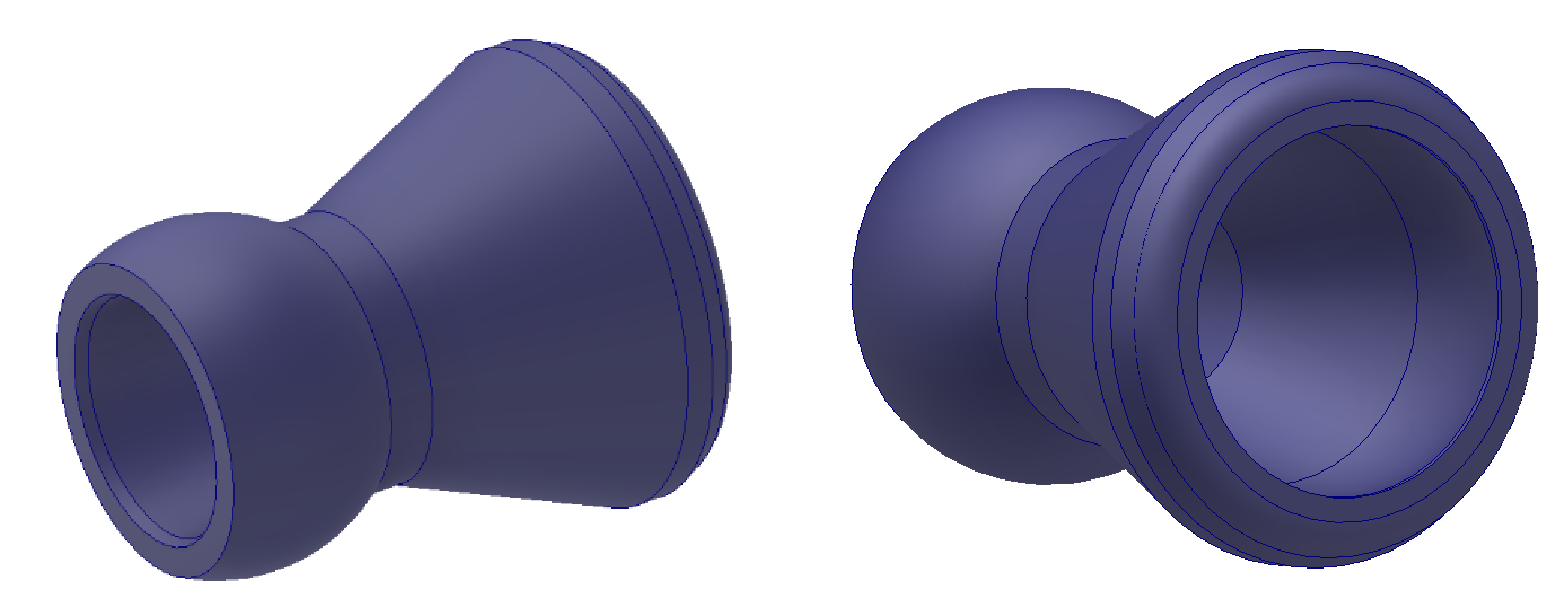
\includegraphics[width=0.8\textwidth]{brazo_1.pdf}
\caption{Elemento Loc-Line.}
\label{fig:brazo_1}
\end{figure}


\subsection{Diseño del case de la pantalla}
El case de la pantalla se puede observar en la Fig.~\ref{fig:exploded_pantalla}. Este case de dimensiones $\SI{43}{mm} \times \SI{49}{mm} \times \SI{21}{mm}$ será impreso en 3D usando también ABS. Para ensamblar las dos partes del case con la pantalla, se inserta la placa electrónica de la pantalla en un agujero con su misma forma en el case inferior de la pantalla. Luego la parte superior del case es ensamblada usando pestañas para el posicionamiento y snap fits para la sujeción.

\begin{figure}[hbt!]
\centering
\begin{subfigure}{.5\textwidth}
  \centering
  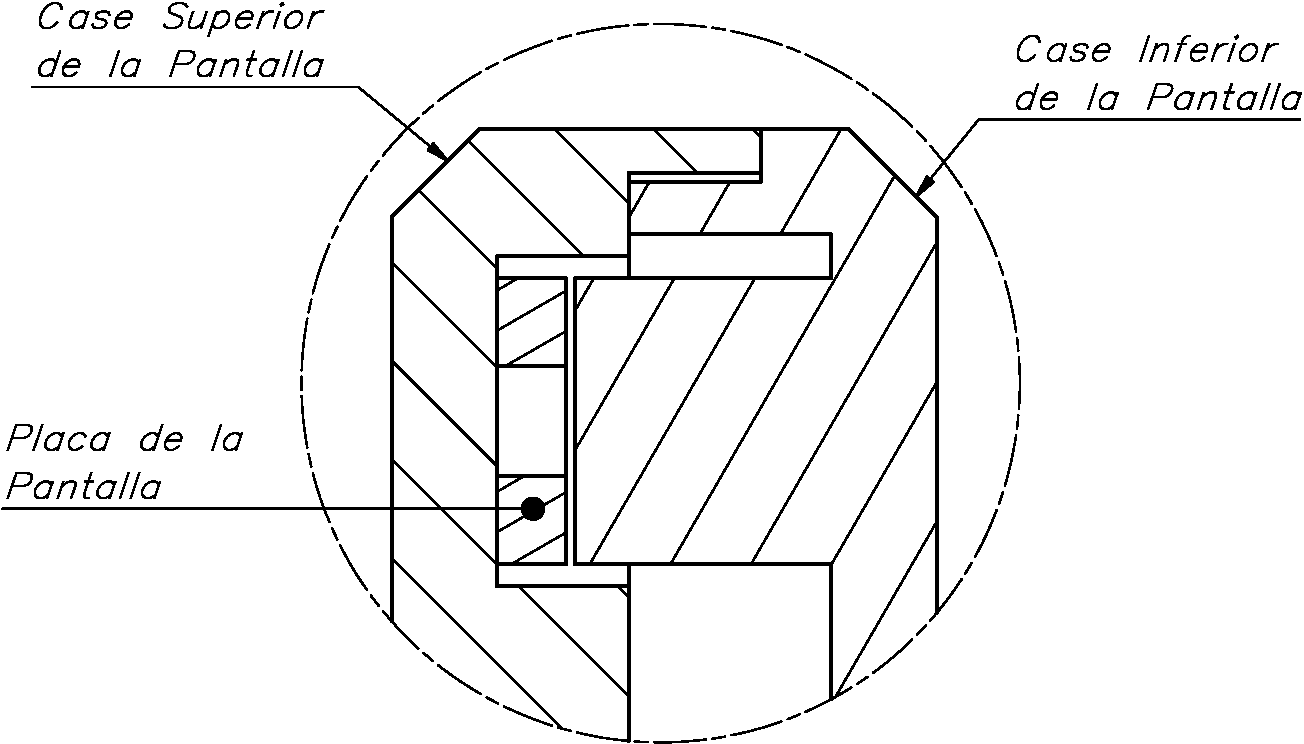
\includegraphics[width=0.97\linewidth]{union_pantalla.pdf}
  \caption{Unión del Case de la Pantalla}
  \label{fig:union_pantalla}
\end{subfigure}%
\begin{subfigure}{.5\textwidth}
  \centering
  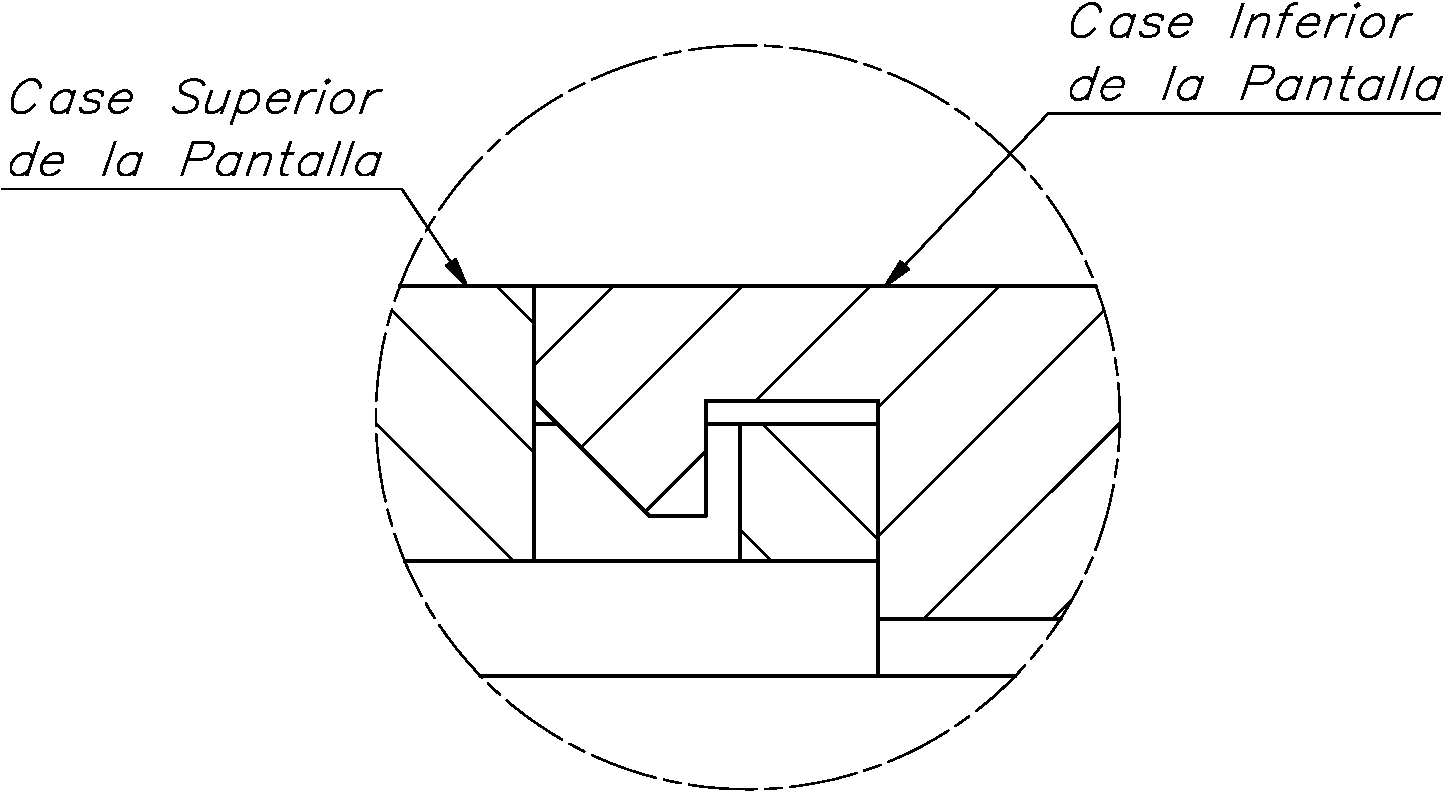
\includegraphics[width=0.9\linewidth]{snap_pantalla.pdf}
  \caption{Snap fit del ensamble del Case de la Pantalla}
  \label{fig:snap_pantalla}
\end{subfigure}
\caption{Detalles del ensamble del case de la pantalla}
\label{fig:test}
\end{figure}


La parte superior del case presiona a la placa electrónica  de la pantalla contra la parte inferior del case usando 4 columnas. Esto se puede observar en la Fig.~\ref{fig:union_pantalla}. Además el snap fit (Fig.~\ref{fig:snap_pantalla}) de este ensamble es distinto del usado en el case principal. En esta ocasión el ángulo de entrada es \SI{45}{\degree} pero el ángulo de salida es \SI{90}{\degree}. Esto significa que la unión es inseparable, ya que el ángulo de entrada permitirá el ensamble y el de salida lo impedirá. Esto se debe a que la pantalla se podrá mover para acomodarse al conductor en cada situación, lo que hace necesario que el case no se separe por error.


\begin{figure}[hbtp!]
\centering
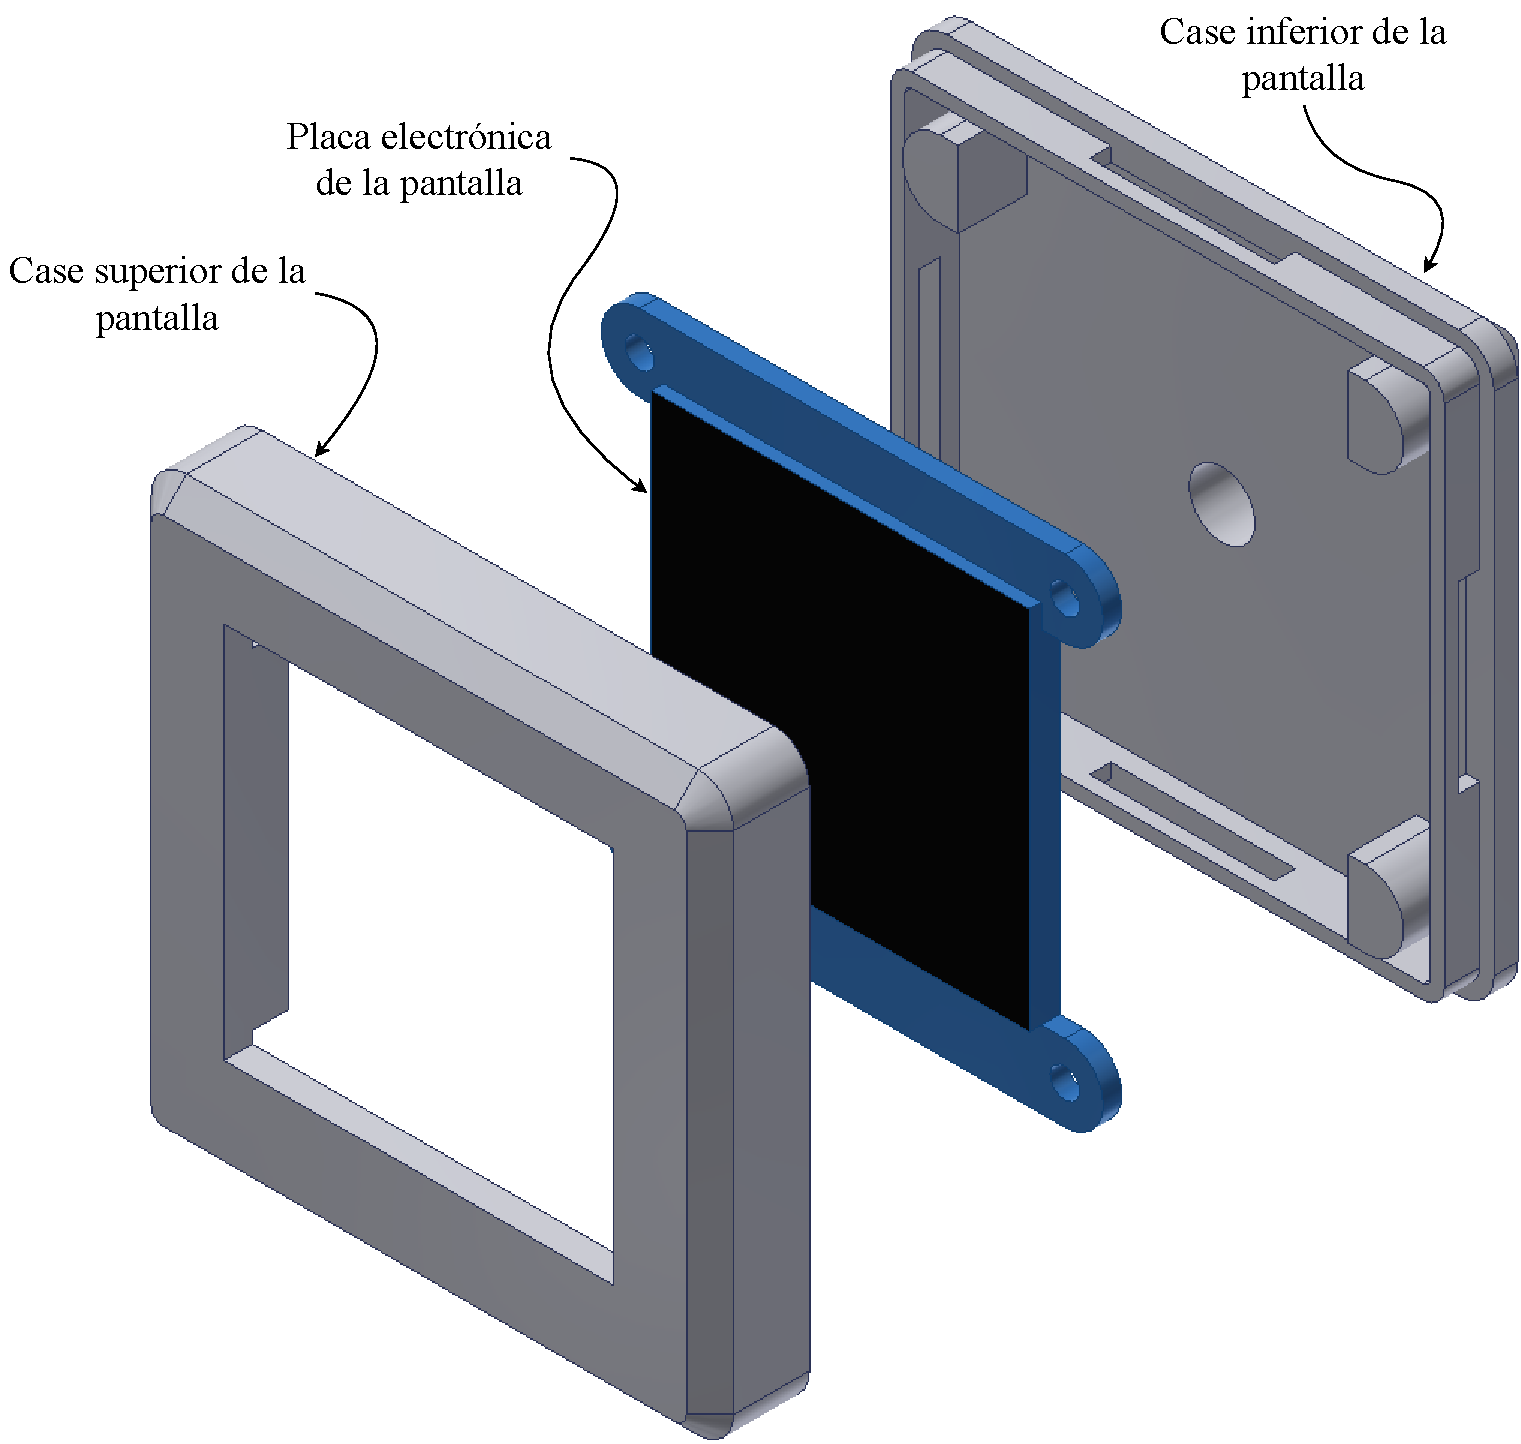
\includegraphics[width=\textwidth]{exploded_2.pdf}
\caption{Vista de explosión del case de la pantalla.}
\label{fig:exploded_pantalla}
\end{figure}

\newpage

\section{Diseño del software de reconocimiento de estilo de conducción}

En esta sección se describe usando diagramas de flujo y pseudocódigo el funcionamiento de la parte de software del sistema de reconocimiento de estilo de conducción. El software consiste en dos partes, la primera se lleva a cabo en cada dispositivo (clientes) y la segunda en un servidor central.

Como se puede observar en la Fig.~\ref{fig:Bloques_software} los clientes envían la información necesaria al servidor central y este clasifica el estilo conducción de cada cliente y los envía de vuelta. Además el servidor mostrará un resumen de los datos recopilados a través de una página web. Los datos mostrados dependen de la persona que inicie sesión en la página. Los conductores podrán ver su puntaje acumulado por día y su historial, y el personal de la empresa podrá ver todos los datos recopilados (Posiciones de los vehículos, consumo, puntaje de los clientes) y resúmenes estadísticos.

\begin{figure}[hbtp!]
\centering
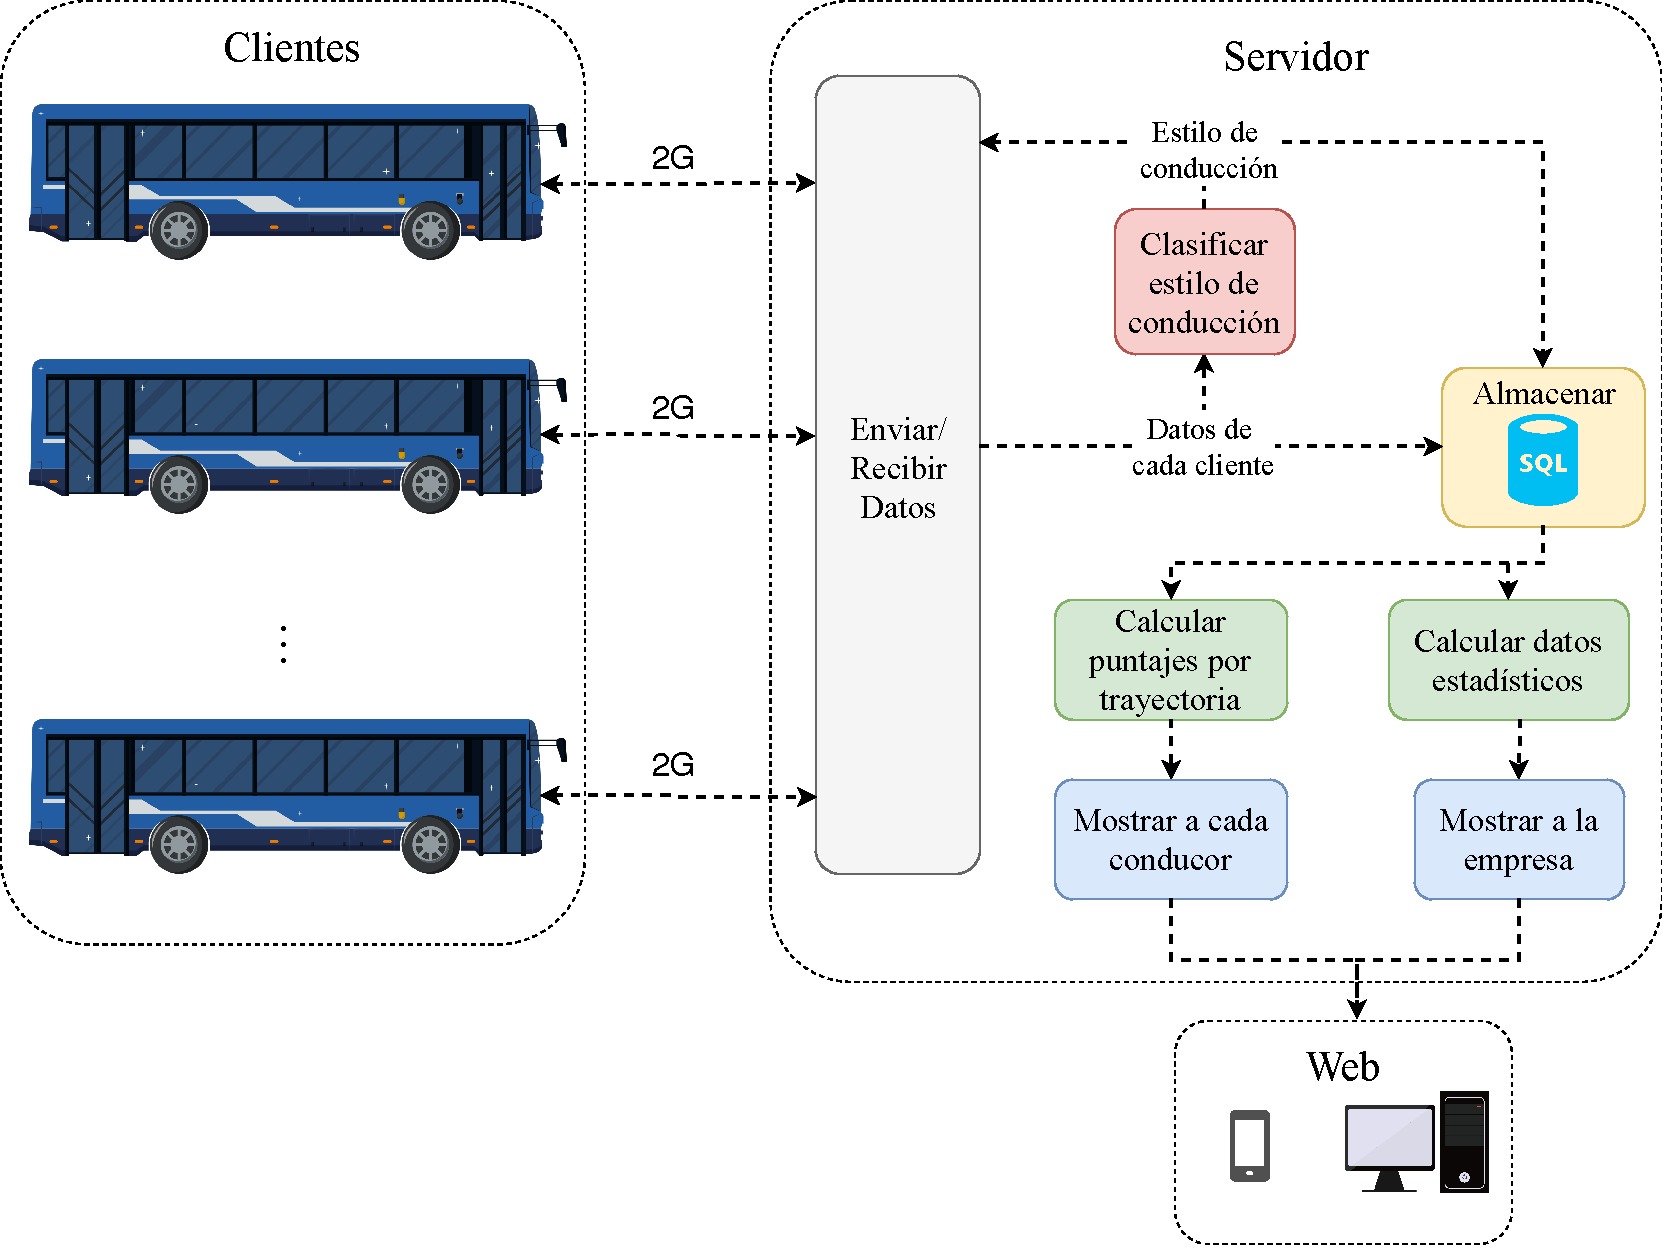
\includegraphics[width=\textwidth]{Bloques_software.pdf}
\caption{Diagrama de bloques del software.}
\label{fig:Bloques_software}
\end{figure}

\subsection{Software de los dispositivos cliente}

Cada dispositivo cliente se coloca en un bus para recopilar datos y enviarlos al servidor. Su funcionamiento se puede apreciar en la Fig.~\ref{fig:Flujo_cliente}. Se inicia el programa al energizar el dispositivo. Luego, este tratará de conectarse al servidor por medio de Internet. Solo al lograr tener una conexión se inicia la recopilación de datos.

El siguiente paso es recopilar los datos de los sensores (IMU, GPS y OBD2). Estos datos necesitan un pre-procesamiento antes de poder ser enviados al servidor. Este pre-procesamiento se lleva a cabo en la función "Sensor Fusion", la cual será explicada más adelante.

A continuación, se almacenan los datos y se repite el proceso durante \SI{1}{s} para luego enviar todos los datos recopilados al servidor. Los datos que se van a enviar se pueden apreciar en la Tabla~\ref{diag:datos_enviar} junto a su tamaño en bytes (Si son representados como texto). Se obtienen estos datos a una frecuencia de \SI{25}{Hz}.

Como se puede apreciar en las Ecuaciones \ref{eq:data_acum1} y \ref{eq:data_acum2}, en \SI{1}{s} de tiempo se acumulan \SI{1625}{bytes}. Estos bytes tardan en enviarse a una velocidad de \SI{85.6}{Kbits/s} a través del módulo 2G solo \SI{0.15}{s}. Luego este ciclo vuelve a repetirse.


\begin{align}
\SI{1625}{bytes}=\SI{65}{bytes}\times\SI{25}{Hz}\times\SI{1}{s} \label{eq:data_acum1} \\
\frac{\SI{1625}{bytes}\times\SI{8}{bits/bytes}}{\SI{85.6}{Kbits/s}}=\SI{0.76}{s}
\label{eq:data_acum2}
\end{align}

\begin{figure}[hbtp!]
\centering
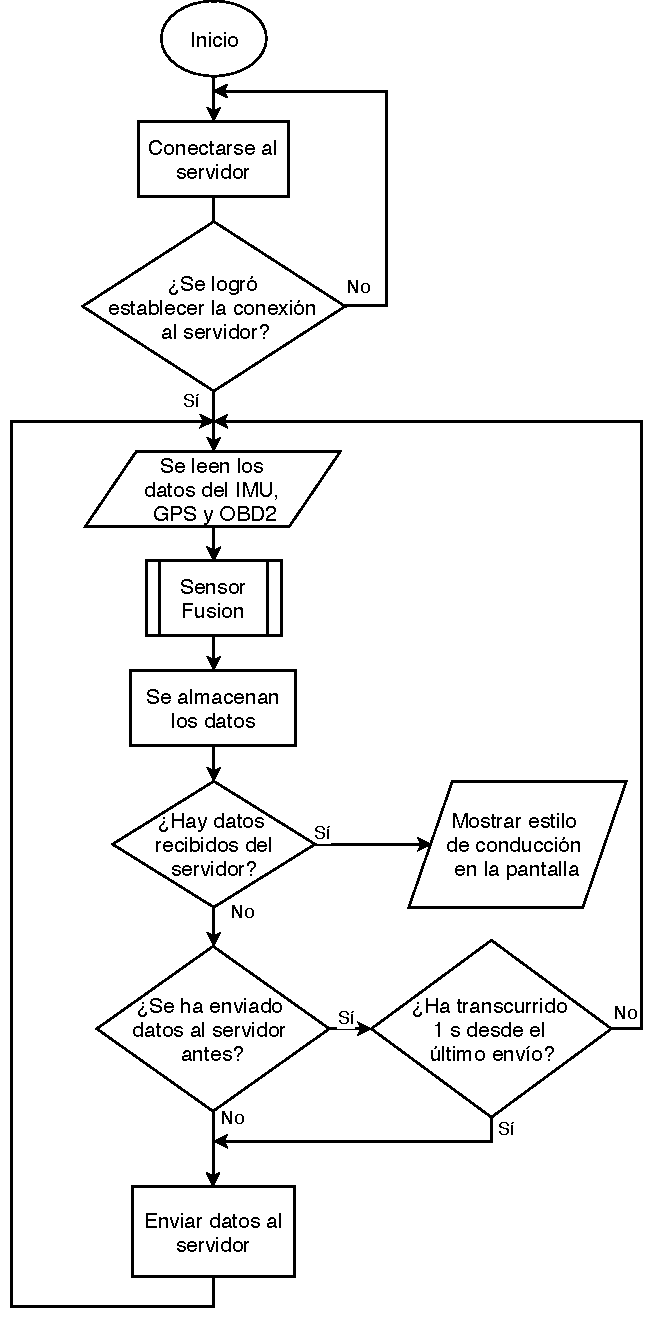
\includegraphics[width=0.7\textwidth]{Flujo_cliente.pdf}
\caption{Diagrama de flujo del software de los dispositivos cliente.}
\label{fig:Flujo_cliente}
\end{figure}

\bgroup
\def\arraystretch{1}%  1 is the default, change whatever you need
\begin{table}[htbp!]
\centering
\caption[Datos a enviar con su tamaño en bytes]{Datos a enviar con su tamaño en bytes.}
\begin{tabular}{ll}
\toprule
Datos & Tamaño en bytes \\ \midrule
Tiempo en ms & 8 \\
Aceleración frontal & 6 \\
Aceleración lateral & 6 \\
Yaw & 6 \\
Latitud & 9 \\
Longitud & 9 \\
Velocidad & 6 \\
RPM & 6 \\
Carácteres separadores & 9 \\ \midrule
Total & 65 \\ \bottomrule
\end{tabular}
\label{diag:datos_enviar}
\end{table}
\egroup

%\subsubsection{Función Sensor Fusion}

\subsection{Software del servidor}

El servidor se encarga de procesar los datos de todos los conductores. Por lo que se tienen varias instancias siendo ejecutadas concurrentemente. Cada instancia esta asociada con un vehículo y conductor. En la Fig.~\ref{fig:Flujo_servidor_principal} se puede observar el proceso que se encarga de administrar las instancias. Luego de crear una instancia para cada vehículo, cuando se cambia de conductor se usa la instancia que ya existía del vehículo usado y se registra el nuevo conductor. Luego se ejecuta la función "Procesar Datos" que se describirá más adelante. Por último, se cierran todas las instancias luego de una hora definida por la empresa.

\begin{figure}[bth!]
\centering
\includegraphics[width=0.55\textwidth]{Flujo_servidor_principal.pdf}
\caption{Diagrama de flujo del software del servidor.}
\label{fig:Flujo_servidor_principal}
\end{figure}

\subsubsection{Función Procesar Datos}
El diagrama de flujo de esta función se puede observar en la Fig.~\ref{fig:Flujo_servidor_procesar}. El primer paso es comprobar si existen nuevos mensajes. Cuando se detecta la presencia de nuevos mensajes se almacenan estos datos y se analizan para detectar el cambio de maniobra.

Cuando se detecta el cambio de maniobra, se ejecuta la función "Clasificar maniobra", que se describirá más adelante. El resultado de esta función es la clasificación del estilo de conducción para la maniobra detectada. Este resultado se almacena y se envía al dispositivo cliente para ser mostrado al conductor.

\begin{figure}[bth!]
\centering
\includegraphics[width=0.3\textwidth]{Flujo_servidor_procesar.pdf}
\caption{Diagrama de flujo de la función Procesar Datos.}
\label{fig:Flujo_servidor_procesar}
\end{figure}

\subsubsection{Función Clasificar maniobra}
Esta función es la encargada de clasificar una maniobra según su estilo de conducción. Como se observa en la Fig.~\ref{fig:Flujo_servidor_clasificar}, el primer paso consiste en extraer todos las muestras de datos que pertenecen a la maniobra. Estos datos van a ser descritos usando características estadísticas para series temporales.

Una vez calculadas estas características, se obtiene por cada maniobra (de varios puntos temporales) una sola instancia . Esta instancia es ahora introducida en el modelo de clasificación que ha sido entrenado previamente. Este modelo nos entregará la clase de estilo de conducción. La etapa del desarrollo del modelo y de su entrenamiento se desarrolla en el Capítulo~\ref{chap:algoritmo}.


\begin{figure}[hbt!]
\centering
\includegraphics[width=0.4\textwidth]{Flujo_servidor_clasificar.pdf}
\caption{Diagrama de flujo de la función Clasificar maniobra.}
\label{fig:Flujo_servidor_clasificar}
\end{figure}


\subsection{Software de la página web}

La página web permitirá visualizar los datos que estén registrados en la base de datos. Como se ha visto en las secciones anteriores, los datos de cada vehículo y cada conductor con su respectivo puntaje y clasificación para cada maniobra son almacenados en esta base de datos. Esta página web tendrá una etapa de autenticación de usuario, en dónde el usuario iniciará sesión. Existirán dos tipos de usuarios: Conductores y Supervisores. La única diferencia es que los conductores solo podrán acceder a los datos registrados consigo mismo y los supervisores podrán acceder a todos los datos disponibles





















\chapter{Algoritmo de clasificación}
\label{chap:algoritmo}

 \graphicspath{{Chapter5/Figuras/}{Chapter6/Figs/PDF/}{Chapter4/Figs/}}

En este capítulo se describirá el proceso de desarrollo del algoritmo de clasificación. Este proceso se puede apreciar en la Fig.~\ref{fig:Flujo_desarrollo}. Además el código completo se puede encontrar en el Anexo \ref{anexo:codigo}.

\begin{figure}[hbt!]
\centering
\includegraphics[width=0.25\textwidth]{Flujo_desarrollo.pdf}
\caption{Diagrama de flujo del desarrollo del algoritmo de clasificación.}
\label{fig:Flujo_desarrollo}
\end{figure}

En la Fig.~\ref{fig:datos_ejemplo} se definen algunos conceptos que se usarán a lo largo de este capítulo. Estos conceptos describen el contenido de un dataset. Cada dataset esta compuesto por \textit{instancias}. Cada instancia tiene un conjunto de \textit{características} y es asignada a una \textit{clase}.

\begin{figure}[hbt!]
\centering
\includegraphics[width=\textwidth]{datos_ejemplo.pdf}
\caption{Partes de un dataset.}
\label{fig:datos_ejemplo}
\end{figure}


\subsection{Recolección de datos}
Como se expresó en el concepto óptimo de solución, se usará en esta tesis un algoritmo supervisado para realizar la clasificación del estilo de manejo. Esto significa que los datos usados para entrenar y validar el algoritmo necesitan estar previamente clasificados.

Debido a la poca disponibilidad de esta clase de datos (datos de manejo clasificados como agresivos o no) se decidió utilizar un dataset disponible en Kaggle, el cuál tenía como objetivo desarrollar una estrategia inteligente para la caja de cambios. Este dataset fue generado usando el puerto OBD2 de un vehículo y un IMU para obtener data durante varios recorridos. Sin embargo, no solo se registró datos de los sensores, sino que también se registro datos categóricos de acuerdo al viaje realizado. En la Tabla~\ref{diag:Dataset} podemos observar todos los datos que contiene este dataset.

\bgroup
\def\arraystretch{1.5}%  1 is the default, change whatever you need
\begin{table}[bth!]
\centering
\caption[Características o features del dataset]{Características o features del dataset.}
\begin{tabular}{@{}ll@{}}
\toprule
Datos de sensores (series temporales) & Datos Categóricos \\ \midrule
Tiempo (segundos) & Número de pasajeros (0 - 5) \\
Velocidad del vehículo (\SI{}{m/s}) & Carga del auto (0 - 10) \\
Número de cambio & Aire acondicionado (0 - 10) \\
Carga del motor (\%) & Apertura de ventanas (0 - 10) \\
Aceleración total (\SI{}{m/s^2}) & Volumen del radio (0 - 10) \\
RPM del motor & Intensidad de lluvia (0 - 10) \\
Pitch  & Visibilidad (0 - 10) \\
Aceleración Lateral (\SI{}{m/s^2}) & Bienestar del conductor (0 - 10) \\
 & Prisa del conductor (0 - 5) \\ \bottomrule
\end{tabular}
\label{diag:Dataset}
\end{table}
\egroup



Como se puede apreciar en la Fig.~\ref{fig:duracion_datps}, estos datos consisten en 39 viajes grabados, los cuales hacen en total \SI{21.5}{h} de manejo grabadas a una frecuencia de \SI{100}{Hz}. Estos datos se usarán para diseñar y probar el algoritmo de clasificación.

\begin{figure}[hbtp!]
\centering
\includegraphics[width=\textwidth]{duracion_viajes.pdf}
\caption{Duración de cada viaje grabado en el dataset.}
\label{fig:duracion_datps}
\end{figure}

Como se observa en la Tabla ~\ref{diag:Dataset}, ninguna de estas características es la clase "agresividad al conducir" o "estilo de conducción". Por lo que se tendrá que definir a que clase pertenecen estos datos. Para esto se una de las características categóricas que se tienen disponibles: "Driver's rush" o "Prisa del conductor".

Cada uno de los 39 viajes ha sido clasificado con un valor de "Prisa del conductor". Se usará este valor como indicador de la agresividad del conductor. Como cada viaje tiene distinta duración, pero mantiene en su toda su extensión el mismo valor de "Prisa del conductor". Se analiza, en la Fig~\ref{fig:numeros_clases}, cuantos datos pertenecerían a cada valor de esta variable.

\begin{figure}[hbt!]
\centering
\includegraphics[width=\textwidth]{instancia_clases.pdf}
\caption{Número de instancias para cada clase.}
\label{fig:numeros_clases}
\end{figure}

Debido a que la presente tesis solo quiere distinguir entre un estilo de conducción agresivo o no agresivo, se agrupan las clases definidas (de 0 a 5) en 2 grupos: el primero agrupando las clases 0, 1 y 2; y el segundo agrupando las clases 3, 4 y 5. Sin embargo, al realizar esta agrupación el número de datos disponible de cada nueva clase difiere mucho el uno de la otra. El primer nuevo grupo cuenta con \num{2182995}, mientras que el segundo con \num{5565758} como se puede observar en la Fig~\ref{fig:numeros_clases_2}

\begin{figure}[hbt!]
\centering
\includegraphics[width=\textwidth]{instancia_clases_2.pdf}
\caption{Número de instancias para cada clase, con clase dividida en 2 grupos.}
\label{fig:numeros_clases_2}
\end{figure}


Si observamos la Fig.~\ref{fig:numeros_clases}, la clase 3 es la que más instancias tiene. Por esta razón se dividirán las 6 clases definidas en el dataset en 3 nuevas clases:

\begin{itemize}
    \itemsep0em
    \item \textit{'Calmado:'} Esta clase se compondrá de las clases 0, 1 y 2.
    \item \textit{'Normal:'} Esta clase será la clase 3.
    \item \textit{'Agresivo:'} Esta clase albergará a las clases 4 y 5.
\end{itemize}

Estas clases se distribuyen de una manera más uniforme como se aprecia en la Fig~\ref{fig:numeros_clases_3}.

\begin{figure}[hbt!]
\centering
\includegraphics[width=\textwidth]{instancia_clases_3.pdf}
\caption{Número de puntos para cada clase, con clase dividida en 3 grupos.}
\label{fig:numeros_clases_3}
\end{figure}

Una vez que los datos se encuentran correctamente clasificados se procede con el siguiente paso, la segmentación de los datos.

\subsection{Segmentación de los datos}

Los datos que se tienen en este momento tienen el nombre de series temporales, debido a que representan la magnitud de una característica a lo largo del tiempo. Pero esto no significa que a cada instante de tiempo le corresponde un estilo de manejo. El estilo de manejo, ya sea \textit{'Agresivo'}, \textit{'Normal'} o \textit{'Calmado'} no se manifiesta en un instante, sino a lo largo de una ventana de tiempo. Esta ventana puede durar varios segundos o hasta minutos.

El siguiente paso para diseñar el algoritmo es lograr segmentar los datos en estas ventanas. Algunos autores toman ventanas de tiempo fijas \cite{6083078}, \cite{4938719}, \cite{8207769}; mientras que otros emplean ventanas que cambian su tamaño dinámicamente \cite{Va-2013}, \cite{6957822}. En esta tesis se usará un tamaño de ventana fijo \textit{\textbf{w}} para la segmentación de datos. El tamaño de la ventana se determinará en la siguientes sección.

\subsection{Extracción de características}

Luego de ser segmentados en ventanas de tiempo, cada una de estas ventanas (compuestas por varios puntos temporales) se tendrá que representar en una sola instancia. Para lograr resumir este conjunto de datos de una manera adecuada, se representará cada serie temporal usando características estadísticas que pueden expresar la información contenida. Estas características estadísticas se muestran en la Tabla~\ref{diag:features}


\bgroup
\def\arraystretch{1.5}%  1 is the default, change whatever you need
\begin{table}[htbp!]
\centering
\caption[Parámetros para series de tiempo]{Parámetros para series de tiempo \cite{Feature_extraction}.}
\begin{tabular}{p{0.5\textwidth}l}
\toprule
\multicolumn{2}{l}{Parámetros estadísticos para series temporales} \\ \midrule
$x_{rms}= \sqrt{\frac{1}{N}\sum_{n=1}^{N} x^{2}(n)} $  &
$ x_{p-p}=x_{max}-x_{min} $  \\
$ S_f=\displaystyle\frac{x_{rms}}{\left|\frac{1}{N}\sum_{n=1}^{N} x(n)\right|} $  &
$ CL_f=\displaystyle\frac{x_{max}}{\left|\frac{1}{N}\sum_{n=1}^{N} \sqrt{|x(n)|}\right|^{2}} $  \\
$ C_f=\displaystyle\frac{x_{max}}{x_{rms}} $  &
$ I_f=\displaystyle\frac{x_{max}}{\left|\frac{1}{N}\sum_{n=1}^{N} x(n)\right|} $ \\
$ K_v=\displaystyle\frac{\frac{1}{N}\sum_{n=1}^{N} x^{4}(n)}{x_{rms}^4} $ \\
\multicolumn{2}{p{\textwidth}}{Donde: \newline
$x(n)$ es una serie temporal para la cuál  $n = 1,2,...,N$ y $N$ es el número de puntos de la serie.}\\
$x_{rms}$ es la raíz cuadrática media. & \\
$ x_{p-p}$ es la amplitud pico a pico. &
$ S_f$ es el factor de forma. \\
$ CL_f$ es el "clearence factor". &
$ C_f$ es el factor de cresta. \\
$ I_f$ es el factor de impulso. &
$ K_v$ es el valor de kurtosis.  \\ \bottomrule
\end{tabular}
\label{diag:features}
\end{table}
\egroup

En el dataset se tienen 5 series temporales, de cada una se obtienen las 7 características mencionados anteriormente. Esto nos deja con un dataset que tiene 35 características por cada instancia. Sin embargo, no todas estas características nos serán útiles para clasificar las instancias en las distintas clases. Es probable que muchas de estas características se encuentren correlacionadas y no aporten información significante.

Además el tener más características hace que el modelo del sistema sea más complejo y esto puede conllevar la generación de \textit{overfitting}. El \textit{overfitting} causa que el modelo entrenado sea muy bueno clasificando los datos con los que ha sido entrenado, pero muy malo clasificando instancias que no ha visto anteriormente.

Debido a esta razón se necesita reducir el número de  características del dataset.

\subsection{Reducción de características}

Existen distintos algoritmos que son usados para la reducción de características.Uno de los más usados es \textit{PCA} o \textit{Principal Component Analysis}. El funcionamiento de este algoritmo se describe en la Tabla~\ref{diag:PCA}


\bgroup
\def\arraystretch{1.5}%  1 is the default, change whatever you need
\begin{table}[htbp!]
\centering
\caption[Algoritmo de PCA]{Algoritmo de PCA \cite{Data_mining_techniques}.}
\begin{tabular}{p{0.9\textwidth}}
\toprule
Principal Component Analysis \\ \midrule
\vspace{-9mm}
\begin{enumerate}
    \itemsep0em
    \topsep0pt
    \item Organizar los datos como una matriz  de tamaño $m\times n$, donde $m$ es el número de características y $n$ es el número de instancias.
    \item Se resta a cada elemento la media de cada característica.
    \item Se calcula la matriz de covarianza.
    \item Se calculan los autovectores y autovalores de la matriz.
    \item Se reordena los autovectores y autovalores en orden decreciente según los autovalores
\end{enumerate}\\ \bottomrule
\end{tabular}
\label{diag:PCA}
\end{table}
\egroup

Luego de ejecutar PCA se tiene un nuevo set de características (resultantes de transformaciones de las características originales). Este set de características esta ordenado de acuerdo a la varianza que cada nueva característica (componente) tiene con respecto a la clase.

\begin{figure}[hbt!]
\centering
\includegraphics[width=\textwidth]{PCA_dist.pdf}
\caption{Varianza para cada componente obtenido a partir de PCA.}
\label{fig:PCA_dist}
\end{figure}

Al dividir los datos usando una ventana $w=\SI{20}{s}$ y aplicar PCA, se obtienen los siguientes componentes o nuevas características. En la Fig.~\ref{fig:PCA_dist} se puede observar el valor de varianza de cada característica. Solo se muestran los 4 primeros componentes, debido a que la varianza de los demás es muy baja.

\begin{figure}[hbt!]
\centering
\includegraphics[width=\textwidth]{PCA_vs.pdf}
\caption{Compontentes gráficados entre sí luego de usar.}
\label{fig:PCA_vs}
\end{figure}

En la Fig~\ref{fig:PCA_vs} se observa la gráfica de cada componente. Se puede notar que los datos no se encuentran totalmente separados. Para solucionar esto se puede usar un algoritmo como \textit{Fast ICA} o \textit{Fast Independent Component Analysis}.





\textit{Fast ICA} necesita de un \textit{prewhitened} de los datos (un preprocesamiento, en este caso se ha realizado PCA) y busca la rotación ortogonal de los datos para lograr una separación entre clases. Luego de aplicar este algoritmo sobre los datos se obtienen 4 nuevos componentes. Se pueden observar estos componentes en la Fig~\ref{fig:PCA_vs_separados}

\begin{figure}[hbt!]
\centering
\includegraphics[width=\textwidth]{PCA_vs_separados.pdf}
\caption{Compontentes gráficados entre sí luego de aplicar Fast ICA.}
\label{fig:PCA_vs_separados}
\end{figure}

El siguiente paso para mejorar los datos es normalizar. La normalización ayuda a muchos algoritmos a tener un mejor desempeño. Los resultados de este proceso se pueden observar en la Fig~\ref{fig:PCA_vs_normalizado}.

\begin{figure}[hbt!]
\centering
\includegraphics[width=\textwidth]{PCA_vs_normalizado.pdf}
\caption{Compontentes gráficados entre sí luego de normalizar.}
\label{fig:PCA_vs_normalizado}
\end{figure}

\subsection{Entrenamiento del algoritmo}

Luego del procesamiento de los datos realizados en las secciones pasadas, es hora de entrenar el modelo de clasificación. Para poder entrenar y luego validar los resultados del modelo entrenado, se realiza una división de los datos. Se divide los datos en \textit{datos de entrenamiento} y \textit{datos de validación}. Se utiliza para este caso un 70\% de los datos como datos de entrenamiento y un 30\% como datos de validación.

Usando los datos anteriores, se entrenaron dos modelos : un modelo de \textit{Random Forest} y un modelo de \textit{Redes Neuronales}. Para generar los modelos se usa la librería \textit{Scikit-learn} \cite{scikit-learn} \cite{sklearn_api}. Los parámetros de cada modelo y sus resultados se pueden observar en las Tablas \ref{diag:param_modelos} \ref{diag:results_modelos}



\begin{table}[htbp!]
\centering
\caption{Parámetros de los modelos entrenados.}
\includegraphics[width=\textwidth]{param_modelo.pdf}
\label{diag:param_modelos}
\end{table}


\begin{table}[htbp!]
\centering
\caption{resultados de los modelos entrenados.}
\includegraphics[width=\textwidth]{results_modelo.pdf}
\label{diag:results_modelos}
\end{table}

Los resultados del algoritmo de la red neuronal son mejores que los de random forest. Las redes neuronales logran clasificar correctamente todos los casos de la clase \textit{Agresivo}. Sin embargo ambos algoritmos fallan al tratar de clasificar las clases: \textit{Tranquilo} y \textit{Normal}

Estos resultados se deben principalmente a la calidad de los datos que se usaron para el diseño. Uno de los factores más influyentes fue el hecho de usar la característica categórica \textit{Prisa del conductor} como clase  de estilo de manejo. Sin embargo, esto no es del todo cierto. En las recomendaciones del Capítulo \ref{chap:Conclusiones} se pronpondrá como recomendación el desarrollo de un experimento controlado, en dónde se pueda adquirir datos de calidad correctamente clasificados.


\chapter{Costos del Sistema}

 \graphicspath{{Chapter6/Figuras/}{Chapter6/Figs/PDF/}{Chapter4/Figs/}}

En este capítulo se presentan los costos del sistema de reconocimiento de estilo de conducción. Se divide en costos de componentes electrónicos y componentes mecánicos (fabricación de componentes y compra de componentes). Además se considera también un costo de envío como un 40\% del costo de los componentes. Este porcentaje representa los gastos de envío y aduanas, entre otros.

\section{Costos de componentes electrónicos}

Se puede observar en las Tablas \ref{diag:costos_elec_1} y \ref{diag:costos_elec_2} la lista de componentes electrónicos que conforman el sistema de reconocimiento de estilo de manejo con sus costos en dólares.

\begin{table}[htbp!]
  \centering
  \caption{Costo de componentes electrónicos (parte 1)}
  \label{diag:costos_elec_1}
  \includegraphics[width=0.9\linewidth]{BOM_1.pdf}
\end{table}

\begin{table}[htbp!]
  \centering
  \caption{Costo de componentes electrónicos (parte 2)}
  \label{diag:costos_elec_2}
  \includegraphics[width=0.9\linewidth]{BOM_2.pdf}
\end{table}

\section{Costos de fabricación y componentes mecánicos}
\section{Costo total}

\chapter{Conclusiones y Recomendaciones}
\label{chap:Conclusiones}


 \graphicspath{{Chapter6/Figuras/}{Chapter6/Figs/PDF/}{Chapter4/Figs/}}


En este capítulo se exponen las conclusiones y recomendaciones generadas al finalizar el presente trabajo. En resumen, en esta tesis se realizó el diseño de un sistema de clasificación de estilo de manejo para empresas de transporte. Para esto se analizaron los tipos de algoritmos más usados, se diseñó el dispositivo que recoge los datos de manejo y se diseñó y validó el algoritmo de clasificación.

El objetivo principal de la tesis fue lograr clasificar el estilo de conducción de un usuario. Como se observó en el Capítulo \ref{chap:algoritmo}, la precisión del algoritmo tiene un margen de mejora amplio. Sin embargo, se demostró que se pueden obtener resultados aún con datos de baja calidad y que es posible clasificar el estilo de conducción de un conductor.

La clasificación de estilo de conducción es el primer paso para lograr un sistema de tránsito más seguro, ordenado y eficiente. Al lograr que las personas usen esta información para mejorar su estilo de conducción permitiría el ahorro de combustible, dinero y un aumento en la seguridad vial. En \cite{vinitsky2018benchmarks} se demostró que insertando un solo auto autónomo con un estilo de conducción adecuado en un ambiente con autos manejados por humanos, se duplicó la velocidad promedio de todos los autos. Esto significa que si las personas mejoran su estilo de conducción; el tráfico, uno de los grandes problemas en Lima, podría disminuir.

Además se tienen las siguientes recomendaciones para futuras investigaciones:
\begin{itemize}
    \itemsep0em
    \item Los datos a usar para entrenar el algoritmo deben ser generados por experimentos controlados con diferentes conductores, rutas y condiciones de manejo, para que se asegure la correcta interpretación de las relaciones de las características con las clases por parte del algoritmo.
    \item Se recomienda también, complementar el reconocimiento de estilo de conducción con tips o indicaciones para el conductor que sirvan para que puedan mejorar su estilo de conducción. Esto se puede implementar usando algoritmos como \textit{LPP} o \textit{learning path planning}.
\end{itemize}






% ********************************** Back Matter *******************************
% Backmatter should be commented out, if you are using appendices after References
%\backmatter

% ********************************** Bibliography ******************************
\begin{spacing}{0.9}

% To use the conventional natbib style referencing
% Bibliography style previews: http://nodonn.tipido.net/bibstyle.php
% Reference styles: http://sites.stat.psu.edu/~surajit/present/bib.htm

%\bibliographystyle{apalike}
\bibliographystyle{IEEEtranN}
\bibliography{References/references}
%\bibliographystyle{unsrt} % Use for unsorted references
%\bibliographystyle{plainnat} % use this to have URLs listed in References
\cleardoublepage
%\bibliography{References/references} % Path to your References.bib file


% If you would like to use BibLaTeX for your references, pass `custombib' as
% an option in the document class. The location of 'reference.bib' should be
% specified in the preamble.tex file in the custombib section.
% Comment out the lines related to natbib above and uncomment the following line.

%\printbibliography[heading=bibintoc, title={References}]


\end{spacing}

% ********************************** Appendices ********************************

%\begin{appendices} % Using appendices environment for more functunality

%%!TEX root = ../thesis.tex
% ******************************* Thesis Appendix A ****************************
\chapter{How to install \LaTeX} 

\section*{Windows OS}

\subsection*{TeXLive package - full version}
\begin{enumerate}
\item	Download the TeXLive ISO (2.2GB) from\\
\href{https://www.tug.org/texlive/}{https://www.tug.org/texlive/}
\item	Download WinCDEmu (if you don't have a virtual drive) from \\
\href{http://wincdemu.sysprogs.org/download/}
{http://wincdemu.sysprogs.org/download/}
\item	To install Windows CD Emulator follow the instructions at\\
\href{http://wincdemu.sysprogs.org/tutorials/install/}
{http://wincdemu.sysprogs.org/tutorials/install/}
\item	Right click the iso and mount it using the WinCDEmu as shown in \\
\href{http://wincdemu.sysprogs.org/tutorials/mount/}{
http://wincdemu.sysprogs.org/tutorials/mount/}
\item	Open your virtual drive and run setup.pl
\end{enumerate}

or

\subsection*{Basic MikTeX - \TeX~ distribution}
\begin{enumerate}
\item	Download Basic-MiK\TeX (32bit or 64bit) from\\
\href{http://miktex.org/download}{http://miktex.org/download}
\item	Run the installer 
\item	To add a new package go to Start >> All Programs >> MikTex >> Maintenance (Admin) and choose Package Manager
\item	Select or search for packages to install
\end{enumerate}

\subsection*{TexStudio - \TeX~ editor}
\begin{enumerate}
\item	Download TexStudio from\\
\href{http://texstudio.sourceforge.net/\#downloads}
{http://texstudio.sourceforge.net/\#downloads} 
\item	Run the installer
\end{enumerate}

\section*{Mac OS X}
\subsection*{MacTeX - \TeX~ distribution}
\begin{enumerate}
\item	Download the file from\\
\href{https://www.tug.org/mactex/}{https://www.tug.org/mactex/}
\item	Extract and double click to run the installer. It does the entire configuration, sit back and relax.
\end{enumerate}

\subsection*{TexStudio - \TeX~ editor}
\begin{enumerate}
\item	Download TexStudio from\\
\href{http://texstudio.sourceforge.net/\#downloads}
{http://texstudio.sourceforge.net/\#downloads} 
\item	Extract and Start
\end{enumerate}


\section*{Unix/Linux}
\subsection*{TeXLive - \TeX~ distribution}
\subsubsection*{Getting the distribution:}
\begin{enumerate}
\item	TexLive can be downloaded from\\
\href{http://www.tug.org/texlive/acquire-netinstall.html}
{http://www.tug.org/texlive/acquire-netinstall.html}.
\item	TexLive is provided by most operating system you can use (rpm,apt-get or yum) to get TexLive distributions
\end{enumerate}

\subsubsection*{Installation}
\begin{enumerate}
\item	Mount the ISO file in the mnt directory
\begin{verbatim}
mount -t iso9660 -o ro,loop,noauto /your/texlive####.iso /mnt
\end{verbatim}

\item	Install wget on your OS (use rpm, apt-get or yum install)
\item	Run the installer script install-tl.
\begin{verbatim}
	cd /your/download/directory
	./install-tl
\end{verbatim}
\item	Enter command `i' for installation

\item	Post-Installation configuration:\\
\href{http://www.tug.org/texlive/doc/texlive-en/texlive-en.html\#x1-320003.4.1}
{http://www.tug.org/texlive/doc/texlive-en/texlive-en.html\#x1-320003.4.1} 
\item	Set the path for the directory of TexLive binaries in your .bashrc file
\end{enumerate}

\subsubsection*{For 32bit OS}
For Bourne-compatible shells such as bash, and using Intel x86 GNU/Linux and a default directory setup as an example, the file to edit might be \begin{verbatim}
edit $~/.bashrc file and add following lines
PATH=/usr/local/texlive/2011/bin/i386-linux:$PATH; 
export PATH 
MANPATH=/usr/local/texlive/2011/texmf/doc/man:$MANPATH;
export MANPATH 
INFOPATH=/usr/local/texlive/2011/texmf/doc/info:$INFOPATH;
export INFOPATH
\end{verbatim}
\subsubsection*{For 64bit OS}
\begin{verbatim}
edit $~/.bashrc file and add following lines
PATH=/usr/local/texlive/2011/bin/x86_64-linux:$PATH;
export PATH 
MANPATH=/usr/local/texlive/2011/texmf/doc/man:$MANPATH;
export MANPATH 
INFOPATH=/usr/local/texlive/2011/texmf/doc/info:$INFOPATH;
export INFOPATH

\end{verbatim}



%\subsection{Installing directly using Linux packages} 
\subsubsection*{Fedora/RedHat/CentOS:}
\begin{verbatim} 
sudo yum install texlive 
sudo yum install psutils 
\end{verbatim}


\subsubsection*{SUSE:}
\begin{verbatim}
sudo zypper install texlive
\end{verbatim}


\subsubsection*{Debian/Ubuntu:}
\begin{verbatim} 
sudo apt-get install texlive texlive-latex-extra 
sudo apt-get install psutils
\end{verbatim}

%%!TEX root = ../thesis.tex
% ******************************* Thesis Appendix B ********************************

\chapter{Installing the CUED class file}

\LaTeX.cls files can be accessed system-wide when they are placed in the
<texmf>/tex/latex directory, where <texmf> is the root directory of the user’s \TeX installation. On systems that have a local texmf tree (<texmflocal>), which
may be named ``texmf-local'' or ``localtexmf'', it may be advisable to install packages in <texmflocal>, rather than <texmf> as the contents of the former, unlike that of the latter, are preserved after the \LaTeX system is reinstalled and/or upgraded.

It is recommended that the user create a subdirectory <texmf>/tex/latex/CUED for all CUED related \LaTeX class and package files. On some \LaTeX systems, the directory look-up tables will need to be refreshed after making additions or deletions to the system files. For \TeX Live systems this is accomplished via executing ``texhash'' as root. MIK\TeX users can run ``initexmf -u'' to accomplish the same thing.

Users not willing or able to install the files system-wide can install them in their personal directories, but will then have to provide the path (full or relative) in addition to the filename when referring to them in \LaTeX.

%\end{appendices}

% *************************************** Index ********************************
\printthesisindex % If index is present

\end{document}
